\chapter{Childhood}

My parents, Francis William and Elizabeth May Russell, were both born
in 1900 and died aged 83 and 90 respectively.

My dad's father owned a shoe shop selling and doing repairs in a small
village called Broughton in Hampshire. He was also a lay-preacher
which was more important to him than his shoes!

I never knew my mother's father for he died when he was 41; a rose
thorn caused him to have blood-poisoning. The poison passed up his arm
and caused a terrible infection. There were no antibiotics in those
days. My mum missed him terribly as she adored him (and he
her). Shortly before he was ill, he told my mum what had happened to
the Titanic. She was twelve years old.

My mum came from farming stock and her brother and mother (a widow)
ran a farm near Romsey in Hampshire and it was there that I spent a
lot of my school summer holidays working on the farm and taking tea
and sandwiches to the men. There was no automatic machinery then so
the farmers had to rely on the marvellous shire horses and manual
labour (including me) to work in the fields. The war took a lot of men
away. My mum left the farm to be a secretary at an office in Swanage,
Dorset and it was there that she met my dad who worked in a rates
office. A paper had to be delivered to his office and she asked to
take it across. Her boss said ``Ah yes, I think you've got your eye on
that nice young man over there!'' They were married in 1922 and my
brother John was born in 1925 followed by me in 1928, my brother Brian
in 1931, and Geoffrey in 1935.

I have no way of remembering anything before I was about five years
and I suppose this is normal. I have a lovely memory of learning to
ride a two-wheeler bike, after getting around on a three-wheeler which
the four of us used. I sat on the bike one day and my brother, John,
guided me round the garden and I suddenly realised I was on my own,
what a thrill! I learned how to tie my shoelaces on the same day. From
that day I lived on a bike -- the whole family rode and even my mother
used to go shopping with a big basket on the front of hers. There was
never enough money for new bikes so when one was needed my dad went to
the market and bought two old ones (for 10~shillings) and would
cleverly put parts together to make one new one, I didn’t realise just
how clever he was; he had a way with repairing sewing machines,
clocks, getting new soles on shoes and he was also a self-taught
organist playing every Sunday in a village church for 42~years. How I
wish I could have given him a pat on the back sometimes -- but I don't
think children are like that.


\chapter{The War}

I was 11 when the Second World War began and I shall never forget the
horror of hearing the bombs coming down. We lived in Hampshire in the
south of England and were surrounded by targets attractive to the
enemy. 47~miles from London we could see the glow of it burning and
the night times were the worst. We had to have special covers made for
the windows for there was not to be a single chink of light. Wardens
had to be on patrol during ``air raid warning red''. What a relief
when the ``all clear'' sounded – a hideous – sounding siren.

We were on rationing, of course, and had to be issued with coupons -
not only for food but for clothes, furniture etc. Rations were poor
but it is said now that if we all ate like that now, we would all be
much healthier. The weekly rations were 2~oz. of sugar,
4~oz. margarine, 2~oz. butter, very little meat, and 1 egg! Having
collected rations for us all my mother would mix the butter and
margarine together (she bought a special pair of butter ``pats''). I
would love this job too! I remember her as being a most practical and
resourceful woman with never a complaint about situations. It must
have been such a worry to bring up 4~kids at this time with the threat
of bombs etc.  but her brother -- my uncle -- a farmer near
Southampton, would send us a chicken or a rabbit skinned and cleaned
for the oven. In those days there were 2~postal deliveries in the day
and what a thrill it was to know there was food coming when that red
postal van stopped outside the house! Nowadays a chicken is everyday
food but then it was a luxury and turned into a nourishing meal for 6!
Good for my mum -- I wish I could have appreciated her more. Why does
one have to have regrets?

Of course, I was too young to join up -- I would have loved to have
been in the WRENS\footnote{Womens Royal Naval Service} but I had a
different kind of war work which was fun. People had to learn how to
deal with broken limbs (as a result of bombings). So I volunteered to
attend twice weekly sessions of being rescued, splintered etc. The
worst part was being showered and carried along draughty corridors on
a stretcher. This operation was to wash off the poisonous gas expected
from the skies; I was never so clean in my life! (The gas never came)
we had to carry gas masks at all times and, when we practiced, we all
looked like pigs!

On Saturday mornings, we children had to go and queue up for saccharin
tablets\footnote{A sugar substitute.} and with long queues, this took
a long time.

On ``Battle of Britain'' day we went to my uncle's farm for the day
and it was only later that we realised it was an historic day. There
was to be an onslaught from the Germans but our wonderful Spitfire
pilots shot down very many of the bombers. In Winston Churchill's
words ``Never has so much been owed by so many to so few''. What a
wonderful man Mr Churchill was. I shall always remember his
encouraging words and messages.

In the midst of all this war nonsense, life had to carry on with
school, work etc. Just at the time when war was declared (Sept 1939),
I started going to Farnham Girls Grammar School. This was to involve a
daily journey (10~miles) starting with a bike ride to the train
station ($1\frac{1}{2}$~miles) and the train ride to Farnham. My bike
went into Mrs Newbold’s shed until I collected it in the
afternoon. She was a wonderful person -- a great friend of my mothers
-- how many times did she hold up the teapot as I went to collect my
bike? There was never any question of a car lift to school or to the
station. I think my dad had a car then but there was severe petrol
rationing. I am pleased to say that even on the icy roads of winter I
never came off my bike! I was not a remarkable pupil at school and was
taken off the clever subjects like latin, math, etc. and put into
domestic science which was not a bad thing because it set me on the
road to my career.

Why I should remember a little man -- the Reverend Tonks -- I have no
idea but memories are made up of people and events. I was fifteen at
the time and my parents agreed that I would play the organ (just a
little Harmonium) at Sunday morning services. I got 10 shillings for
each service -- I was rich indeed! It was winter and I had to cycle
six miles through ice and snow to get to a village called Newton
Valence. Just outside my home town of Alton, Hampshire. But Mr. Tonks
was a character (almost Dickensian) and I remember that he wore white
socks under his priestly robes!

At the services, there were only three people -- himself, the church
warden, and me and, since it was decreed, we had to worship; I am not
sure if he preached a sermon. He was such a jolly little man and I am
sure the Lord was pleased with him; he deserved a larger congregation
but who could blame anyone for not turning out in that awful weather.


\chapter{Adulthood -- Gloucester}

To pursue my best interests, it was decided that I should ``do''
domestic science (today it is called home economics) and this involved
studying all aspects of home management (two years) and then followed
a short course in cookery demonstrating which I passed without
difficulty. In fact I loved it and found it interesting that the more
nervous I felt before a demonstration the better the result (I
understand this theory applies to other aspects of performance, for
example acting). I did not enjoy my demonstration exam. The subject
was the use of soya (of all things!). The main reason was that those
in front of me were fellow students who were prepared to giggle and
take the mickey. However, all went well and I passed out (not
literally). The whole time I was at the domestic science college in
Bath was wonderful and I made good friends, some of whom of course
have passed away. But how perceptive it was of my parents not to
persuade me to pursue anything academic -- a lost cause anyway!

After training college in Bath, I took up a position as home service
adviser, first of all in Luton and then in Gloucester for 6 years. It
was a wonderful life and I was full of bounce and confidence (see
Picture~\ref{madge-adult})!

\begin{figure}
  \centering
  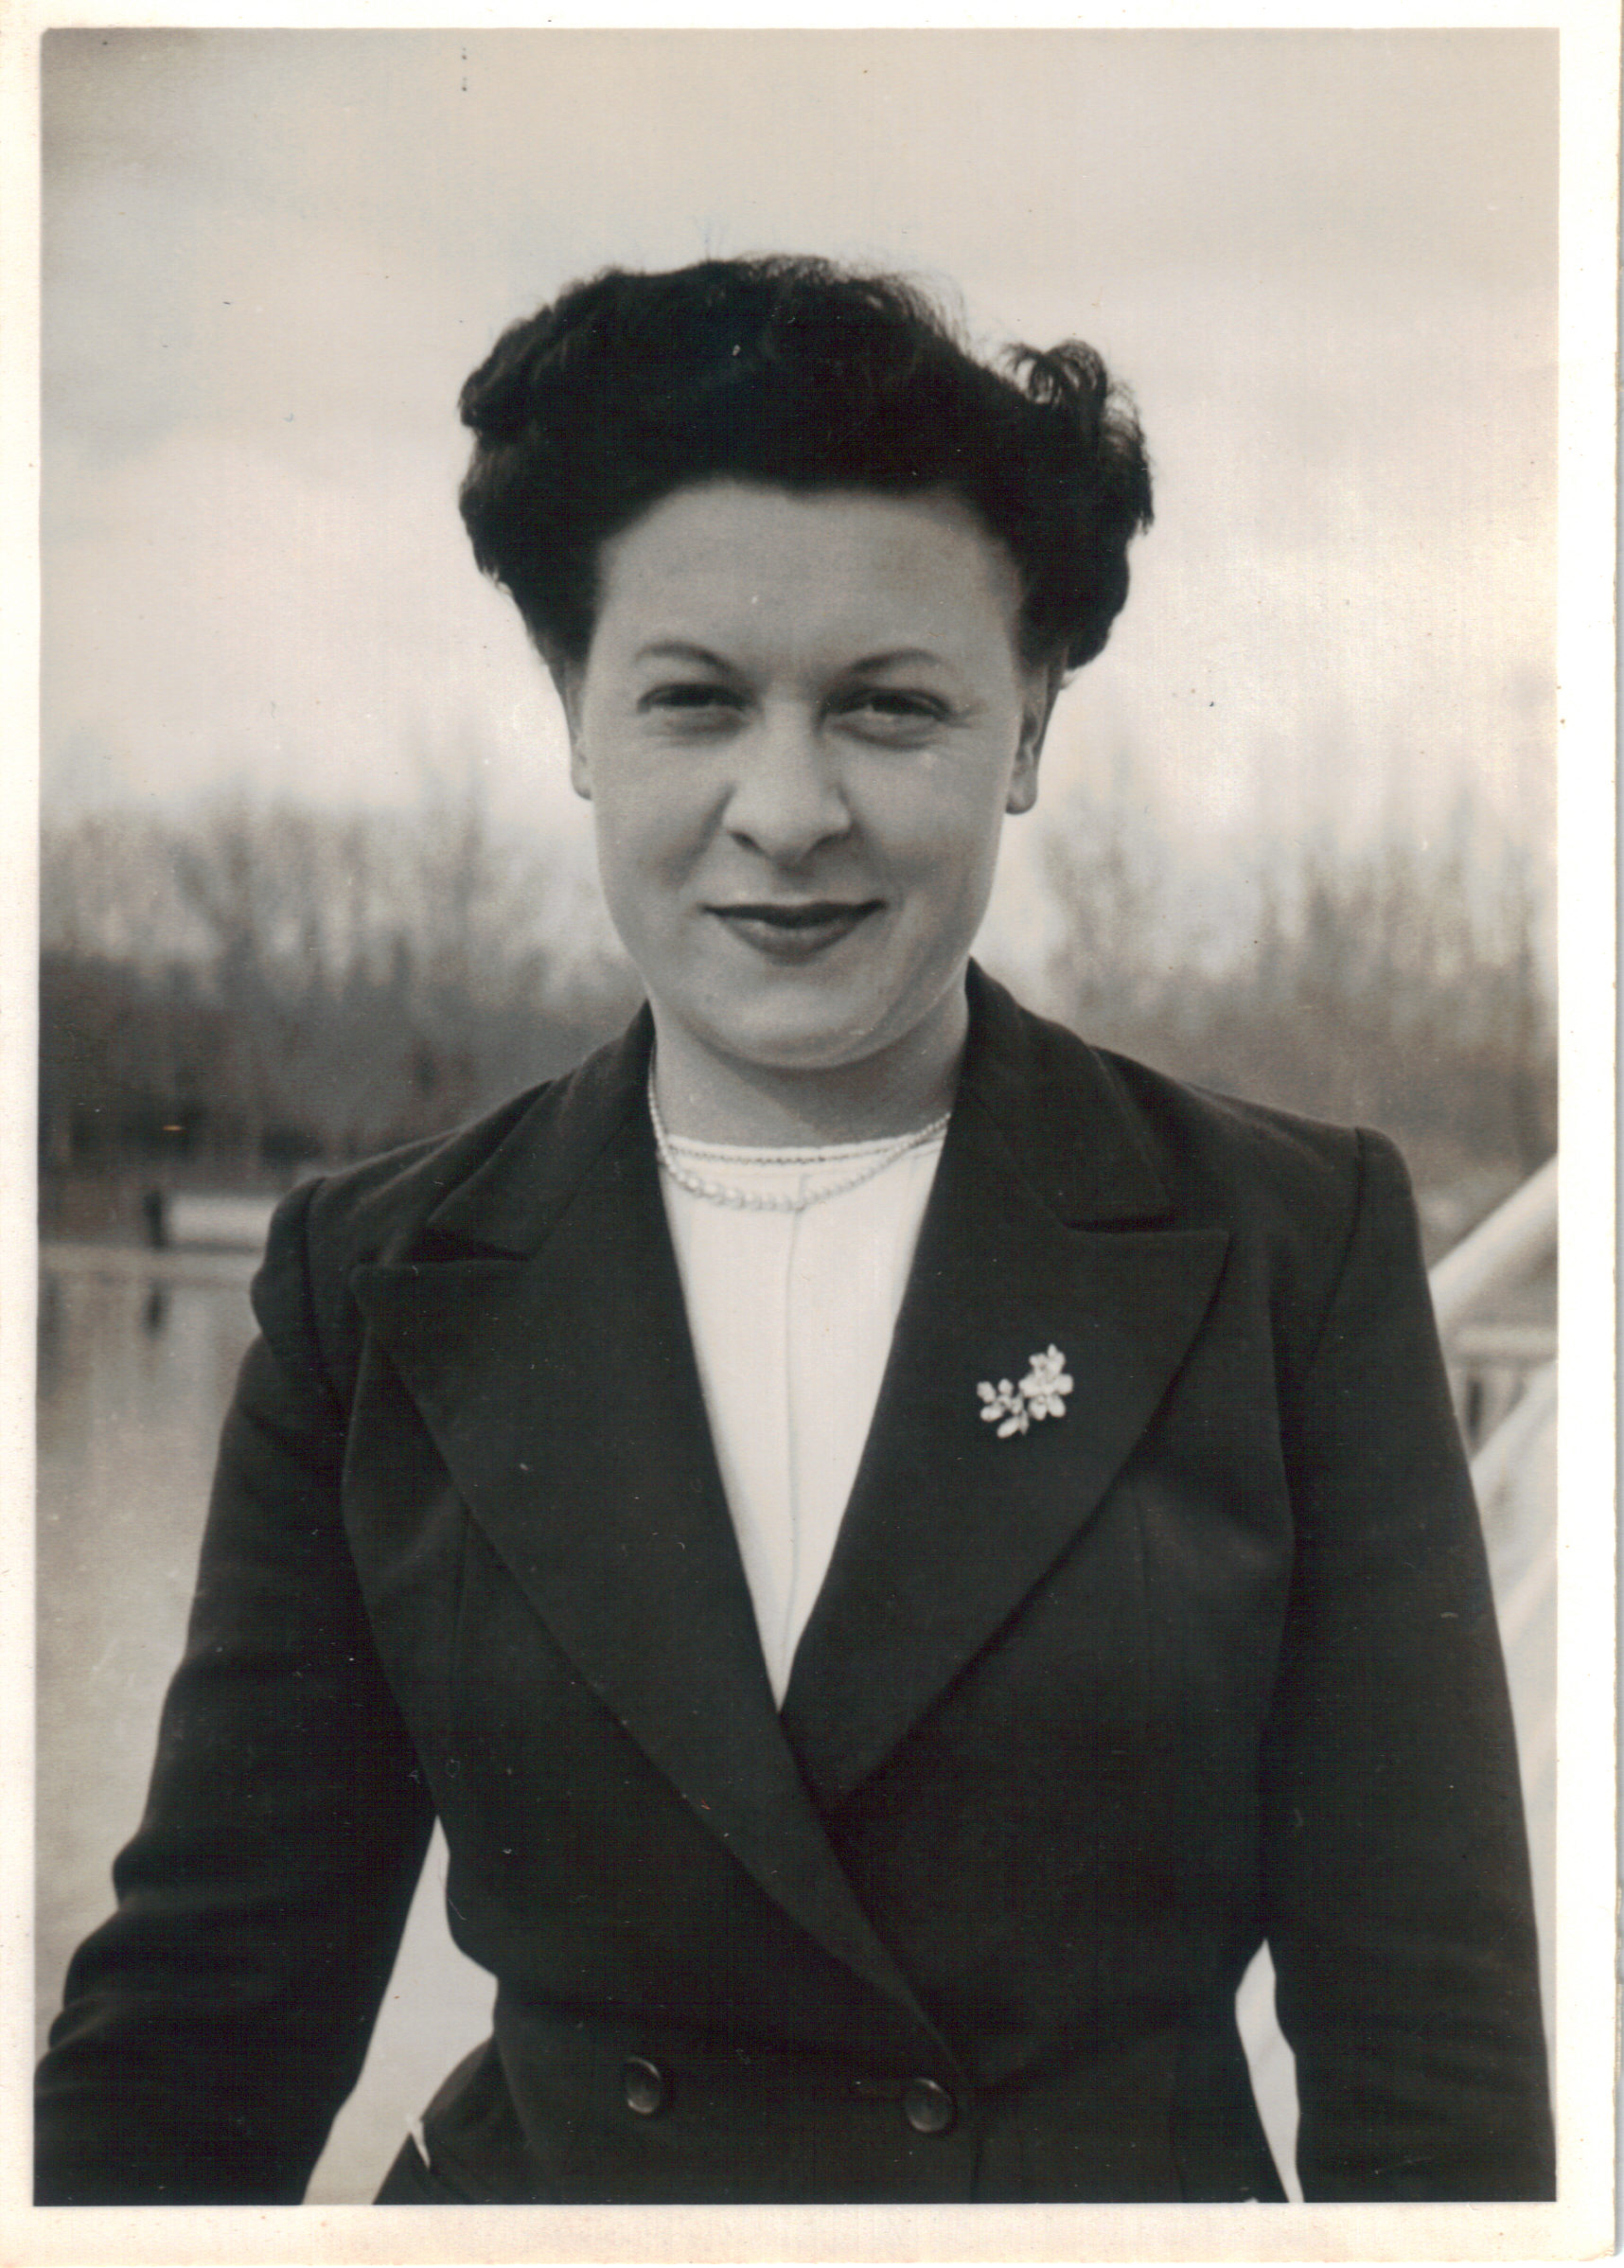
\includegraphics[width=0.95\textwidth]{photos/madge-adult.jpg}
  \caption{My first glimpse of Turkey (1953).}
  \label{madge-adult}
\end{figure}

I was with the gas company and we had a beautiful demonstration
kitchen where we held regular ``dems''. Going out into the country to
talk to women's organisations was more difficult as I had to catch a
bus loaded with my equipment. It was however, lots of fun especially
when things went wrong (for example, failure to add some ingredients,
like baking powder).

These days one would be provided with a car! But it was useful to have
to sign off on a country expedition in order to catch the bus back to
Gloucester because if anything went wrong with the demonstration I was
able to say ``you see what will happen to you if you do not take care
of preparation -- in any case I have a bus to catch now''. What a
career! Demonstrations on TV these days are so much more sophisticated
-- but I am appalled that the clever and deft top class demonstrators
do not tie back their hair -- there is too much hair falling about and
it was always the rule that it should be kept out of the way of
food. But oh! What lovely delicacies they produce.

Because of the war (which was then over) there was not much food to
demonstrate with and I had to resort to things like parsnip pastry
(!), potato scones (!), fat-less sponges, etc. I marvelled at the
confidence I had; with age it dwindles away.

I have always been interested in acting and the theatre and was in
several plays at school. I was good at ``learning by heart'' and could
learn the other actors' words as well as my own. The thrill of the
curtain going up was always tremendous and I believe that the nervous
sensations felt at this moment can be felt by top performers as well
as by amateurs and, in fact, I can relate to this by my feelings when
I was due to begin a cookery demonstration many years later in
Gloucester; if I did not feel sick with nerves and wish I were a
million miles away the demonstration would not go well. In these
circumstances, one has to win the audience over in the first minute
and ``make \'em laugh'' -- then all should go well.

Whilst in Gloucester, I joined an amateur operatic and dramatic
society -- known as ``The Gods''.

The society put on many delightful shows and I loved taking part in
the dramatic side of things -- although I did have a ``walk-on'' part
in ``The Quaker Girl.'' In one comedy (heaven knows which one) I had
to appear briefly in my underwear and shout ``Flags for the
lifeboats.'' It was hilarious! There would sometimes be a bouquet for
me at the closing curtain of a show. No matter that it might be from
someone anonymous -- the thrill and the glamour were there.

The gas company where I was working in Gloucester started a concert
party and I was invited to join as the resident pianist (we called
ourselves ``The Thermites.'' I ask you!).

My gift of being able to play the piano ``by ear'' came in very
useful. We had so much fun doing sketches etc. We would go out into
the country and our audiences showed their appreciation for good,
clean fun and would often provide us with lovely refreshments after
the show! In one particular cold and draughty church hall, the piano
was tied up with pieces of string but it still gave out a good sound!
There was nothing professional about us but we had such a good
time. In the middle of all this I left to get married -- I don't know
if they found another pianist!

I was lucky to become friendly with Alma and John Hoare. John worked
in the gas company's office. I spent every weekend with them; weekends
are the hardest when living alone. I shall always remember their
kindness and hospitality. One Sunday morning, Alma told me they were
to have a visitor -- a young man on leave from Turkey.


\chapter{Love}

\begin{verse}
``In 1952 one day, into my life came Mr Bray''
\end{verse}

If ever anyone tries to argue that there is no such thing as love at
first sight refer them to me!

I was demurely sewing in the lounge when I heard his voice and then
seeing Tony, my pulse raced. In that moment I knew that this was the
man with whom I wanted to spend the rest of my life. He was so
handsome and charming but best of all, I noticed his highly polished
tan colour boots, Oh golly! I think I almost fell in love with his
boots! We exchanged the minimum of greetings but I had seen enough.

He asked me out seven times before he had to return to Turkey but
during that time, we had agreed to marry... On a moonlit drive (in his
hired car) I did a very daring thing and told him I had something to
confess. He must have had a host of thoughts. I told him that I had
fallen in love with him! Everything came together for us and I
couldn't bear the thought of him going away but he had to return to
Turkey and his telecommunications job.

\begin{figure}
  \centering
  \includegraphics[width=\textwidth]{photos/madge-wedding.jpg}
  \caption{Tony and Madge on their wedding day (June 20, 1953).}
  \label{madge-wedding}
\end{figure}

Tony was not close to his parents and I think that was because his
mother kept herself apart. Tony called her ``Fan'' and his father
``Reg''. Reg was a perfect darling and was very fond of me. Tony was
one of a twin but his sister, Pamela, died when she was nine days
old. I thought that when Tony met me Fan would have a good opportunity
to look upon me as her lost daughter but she did not take to me -- in
fact, she disliked me and resented my taking Tony away from her. I did
everything I could to help her, especially when she fell off a bus and
broke her leg -- she had to wear a caliper which was a terrible
impediment. Reg was very kind to me and reckoned I was a ``good
catch''. He died when he was 69 and I lost a good friend and ally.

I took the children to stay with Fan when we were on leave from
Nigeria and worked really hard. She never 100\% took to Elizabeth and
did not recognize Richard! It must be awful to harbour such feelings
against someone as she did to me. I have forgiven her but it would
have made life so much more pleasant had we been on friendly terms. We
did not go back to England when she died. Instead we went and sat in
the church in Lagos at the time of the funeral. I noticed that Tony
did not cry as he did when his father died. I hope Fan is happy in her
afterlife and I wonder if I shall meet her.

There were promises to write but he fell short of this because of the
demands of his job. However glorious arrangements of flowers would
arrive and helped me to forgive him. We had met in January and in
December he asked me to fly to Turkey (and paid my fare -- 100~pounds
-- a lot of money in those days) so I had the opportunity to see the
country where I was to live for three years after our wedding in June
1953. It was my first experience of being overseas and so different
from life in England. The train journey from Istanbul to Ankara (13
hours on the wagon lits) was so romantic and different. I was
transported to another world. Leaving him after the two weeks holiday
(I stayed in the flat where Tony lived with a colleague and his wife)
was unbearably sad. But, after a while I began to enjoy the flight
home. I was the only passenger on the leg from Istanbul to Athens and
was invited to go up front with the crew. I remember laddering a
stocking then! On the poor old Viking aircraft (which was actually a
very reliable plane) we had to have a nights stop in Rome and I was
taken round to see the sights by this very friendly crew.

Life had to return to normal after arriving in England but what a
wonderful memory Turkey was. And what a lot I had to look forward to.

Six months of waiting and planning followed and preparations were made
for our wedding. I went to London to meet Tony on his return from
Turkey and we had a few lovely days on one of which we went to Charles
Packer in Regent street to choose the engagement ring -- a lovely
three stone diamond ring. I was so excited!

Our wedding was a great occasion and held in the assembly rooms in
Alton (see Picture~\ref{madge-wedding}). I could not help thinking of
those other dark days of the war when, in the lower regions of this
building I had been carried on a stretcher to be splinted and bandaged
and showered and carried along the draughty corridors.

We were due to have a honeymoon in Cyprus but there was trouble there
and, after a few days in Haslemere, we flew direct to Turkey. The old
house we stayed in at Haslemere (the house was called ``Undershaw'')
had been owned by Sir Arthur Conan Doyle who was the creator of
Sherlock Holmes and his murder mysteries. Occupied now by old ladies
living out their quiet days of retirement. They took no notice of us
-- or, if they did, they may have guessed that we were on honeymoon
and might have recalled those blissful days of their own. I well
remember the spirit lamps on their breakfast tables to keep the tea
hot!

% \begin{figure}
%   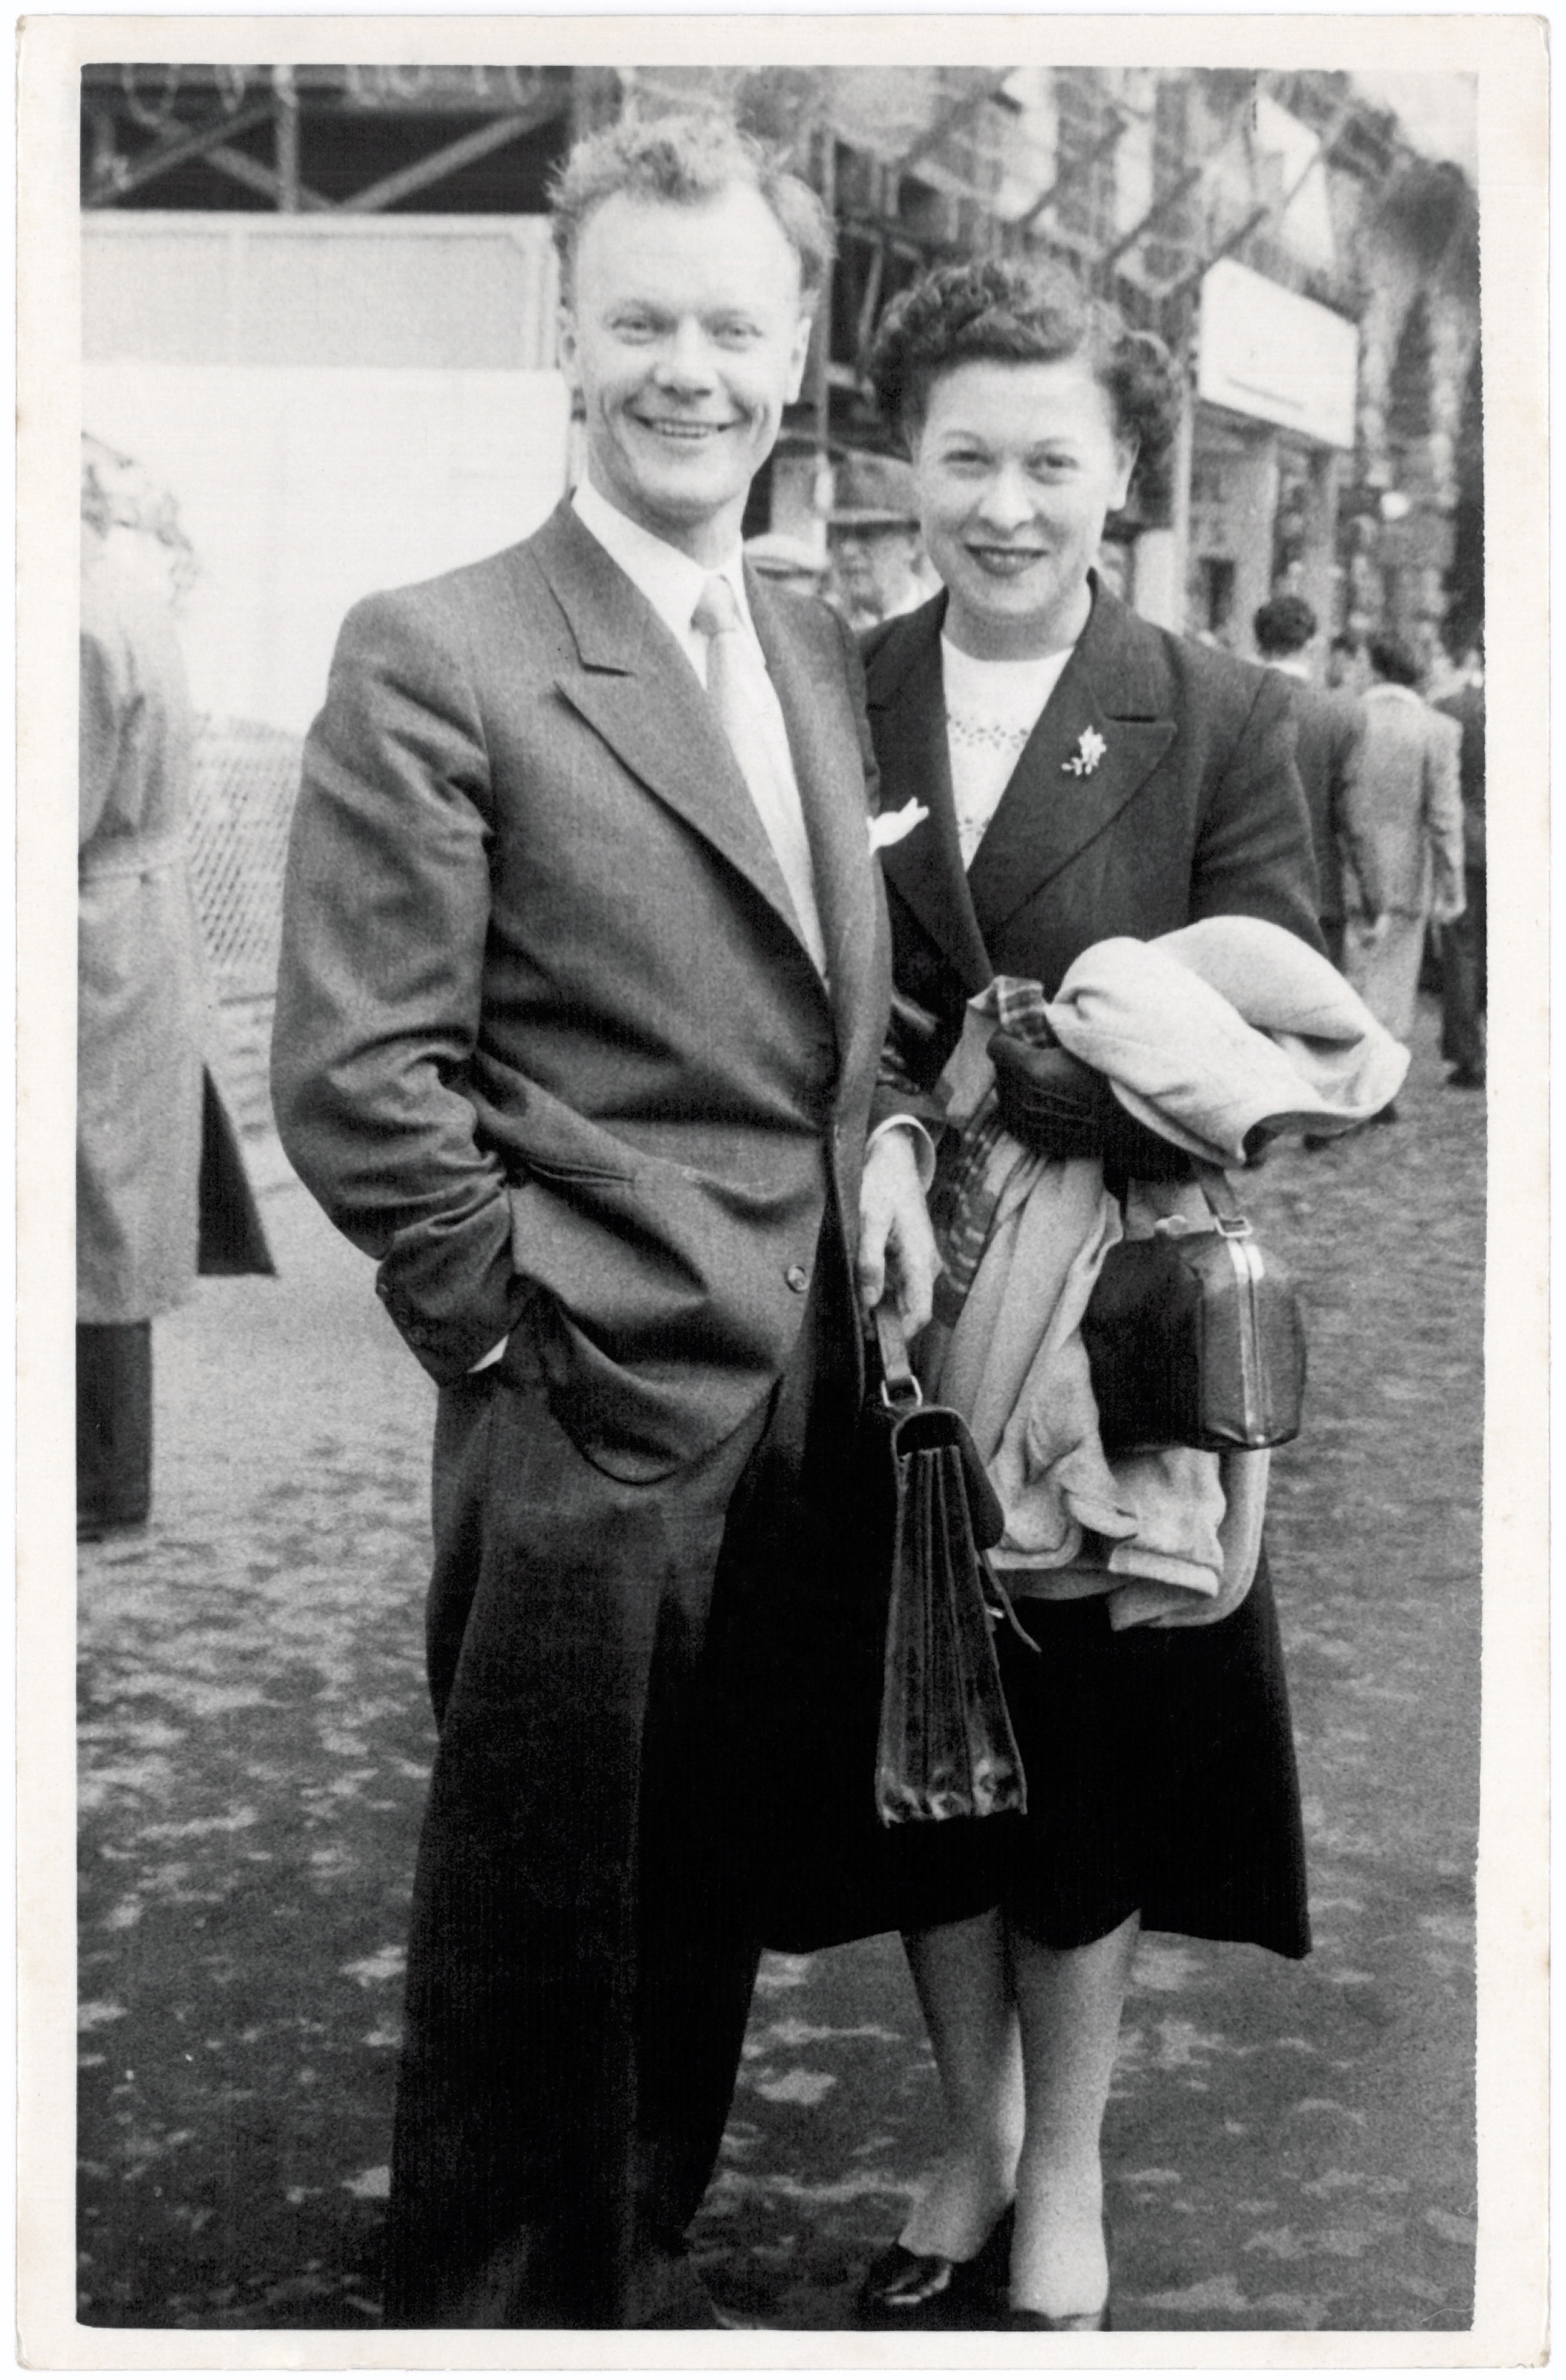
\includegraphics[width=\textwidth]{photos/tony-and-madge3}
%   \caption{Tony and Madge 3.}
%   \label{tony-and-madge3}
% \end{figure}

% \begin{figure}
%   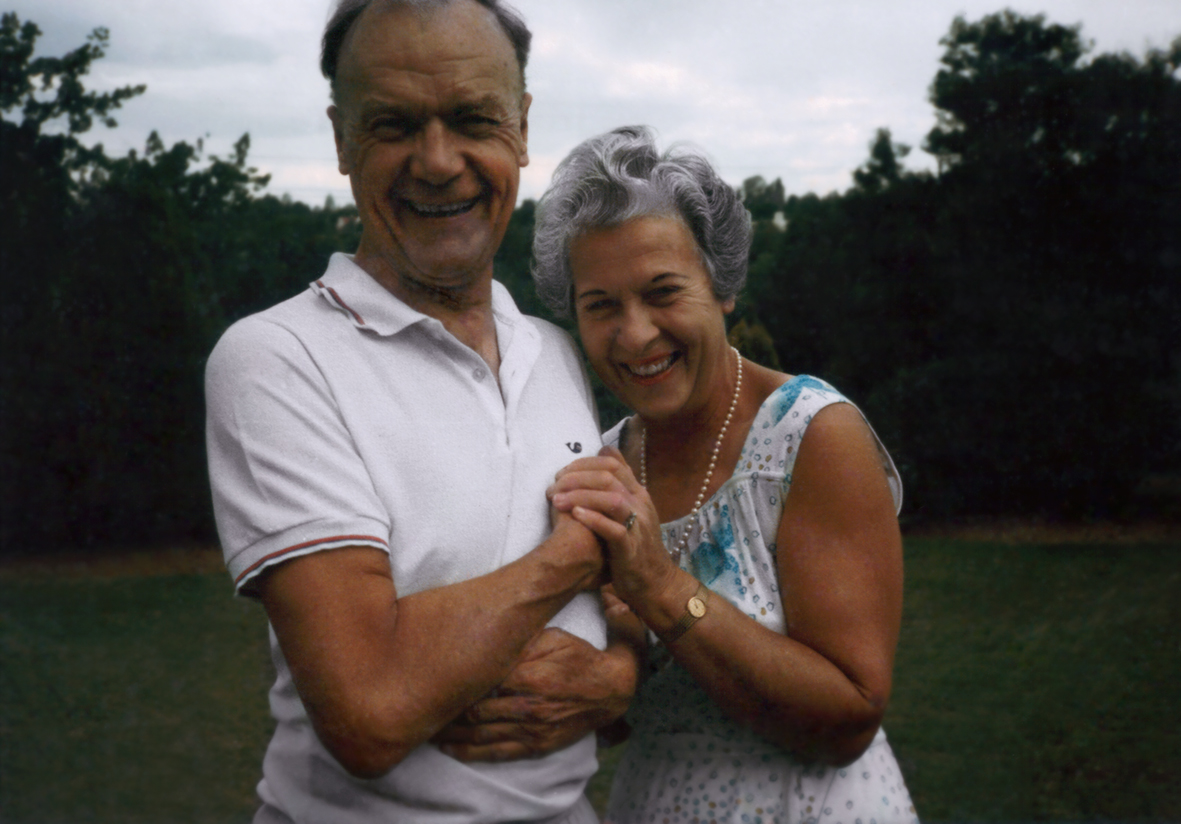
\includegraphics[width=\textwidth]{photos/tony-and-madge2}
%   \caption{Tony and Madge together (19xx).}
%   \label{tony-and-madge2}
% \end{figure}

% \begin{figure}
%   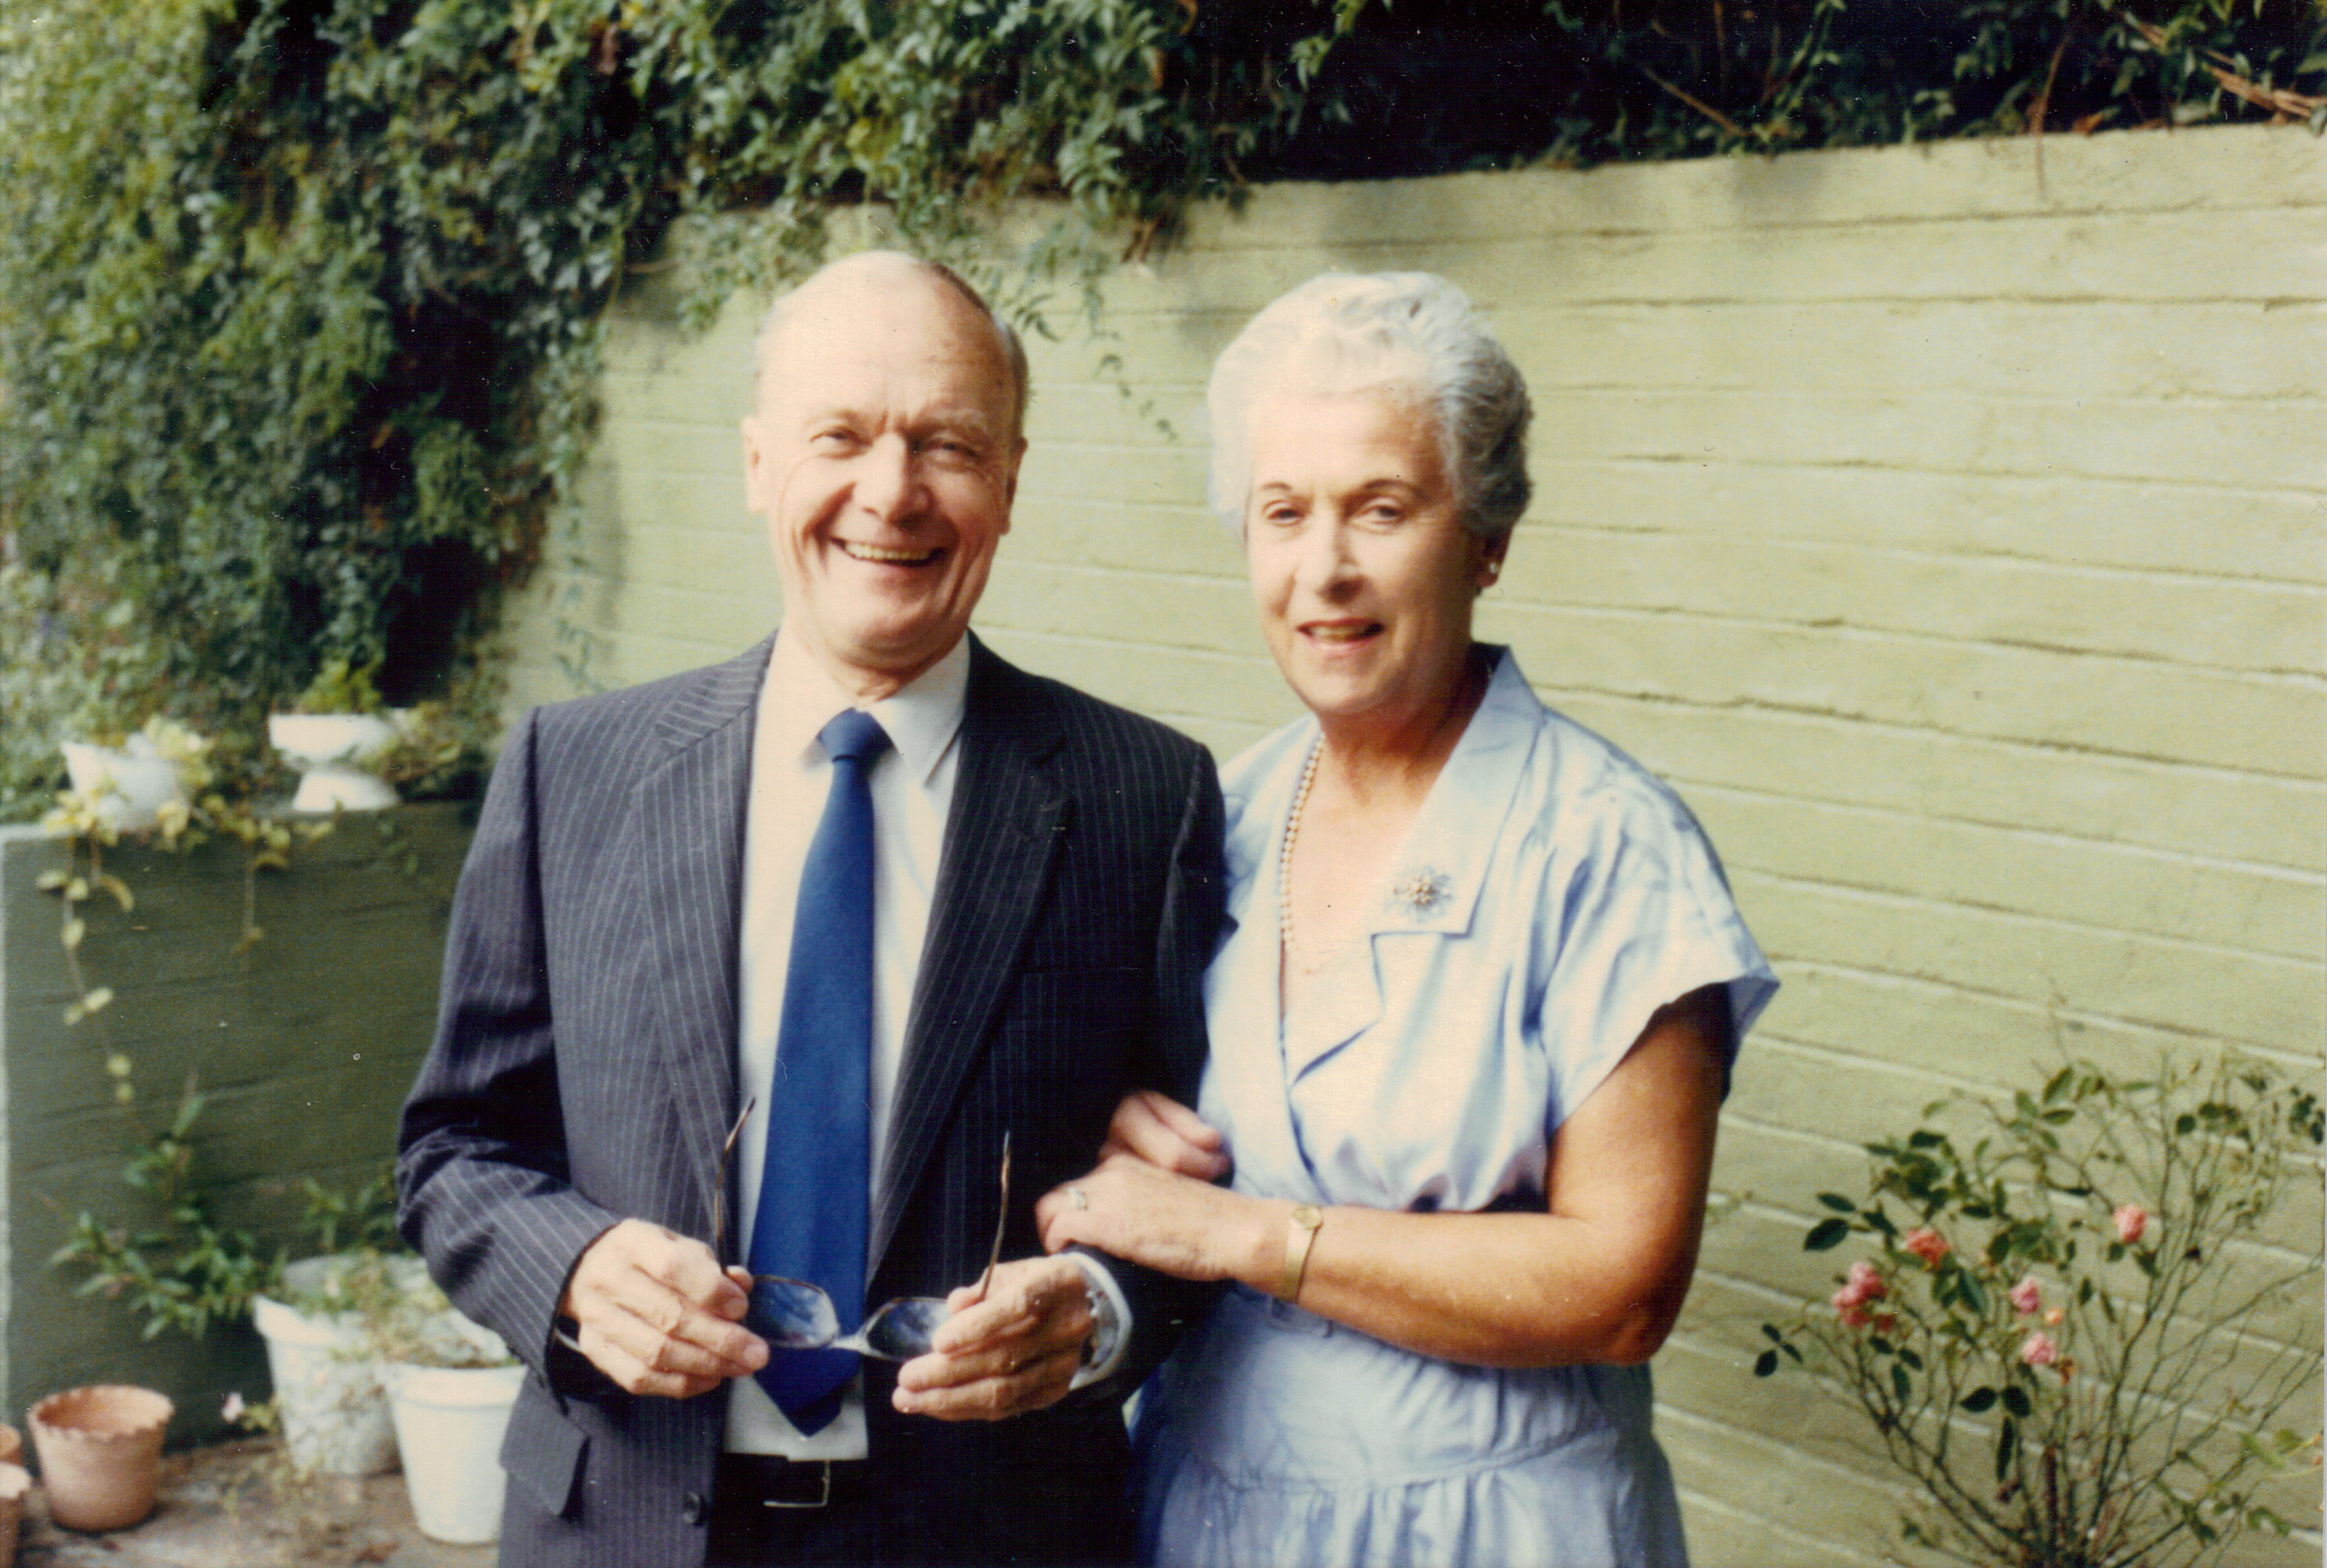
\includegraphics[width=\textwidth]{photos/tony-and-madge}
%   \caption{Tony and Madge together (19xx).}
%   \label{tony-and-madge}
% \end{figure}
\begin{figure}
  \centering
  \begin{tabular}{cc}
    %\multirow{-2}[41]{*}{   % For a4 paper
    \multirow{-2}[32]{*}{    % For letter paper
      \subfloat[In London buying the ring.]{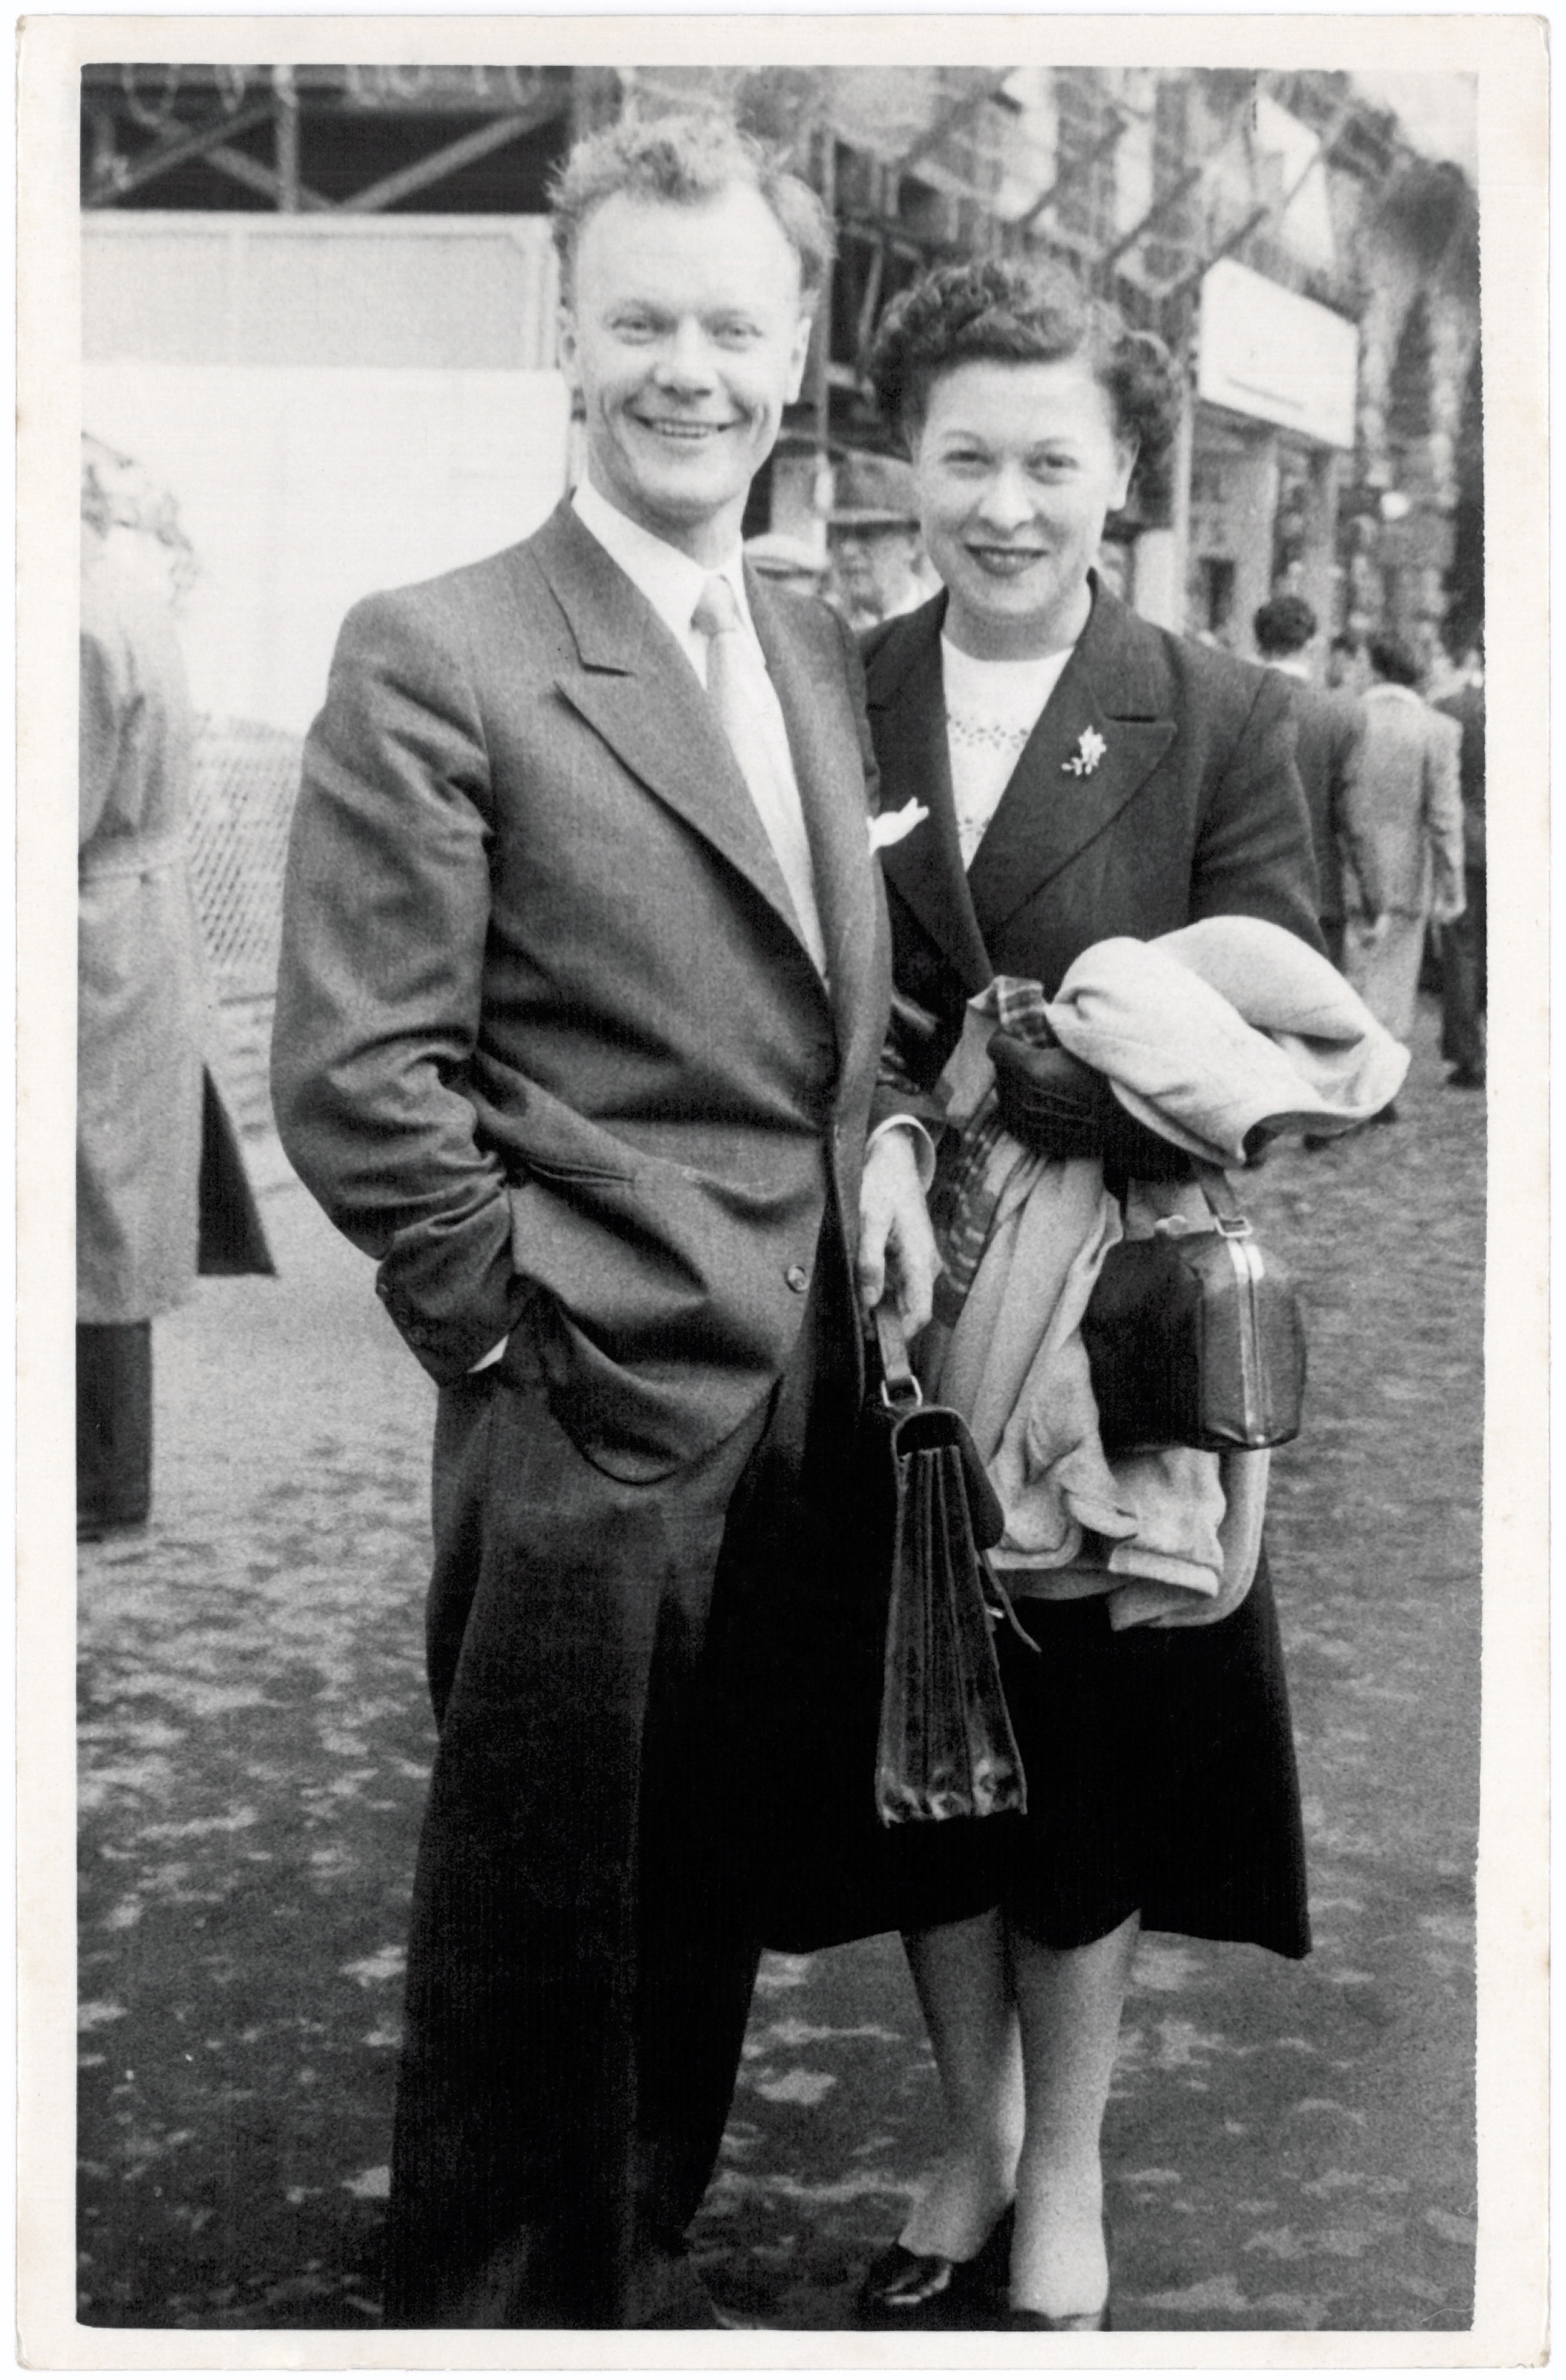
\includegraphics[width=0.45\textwidth]{photos/tony-and-madge3.jpg}\label{tony-and-madge3}}
    } &
    \subfloat[Bryanston (1980).]{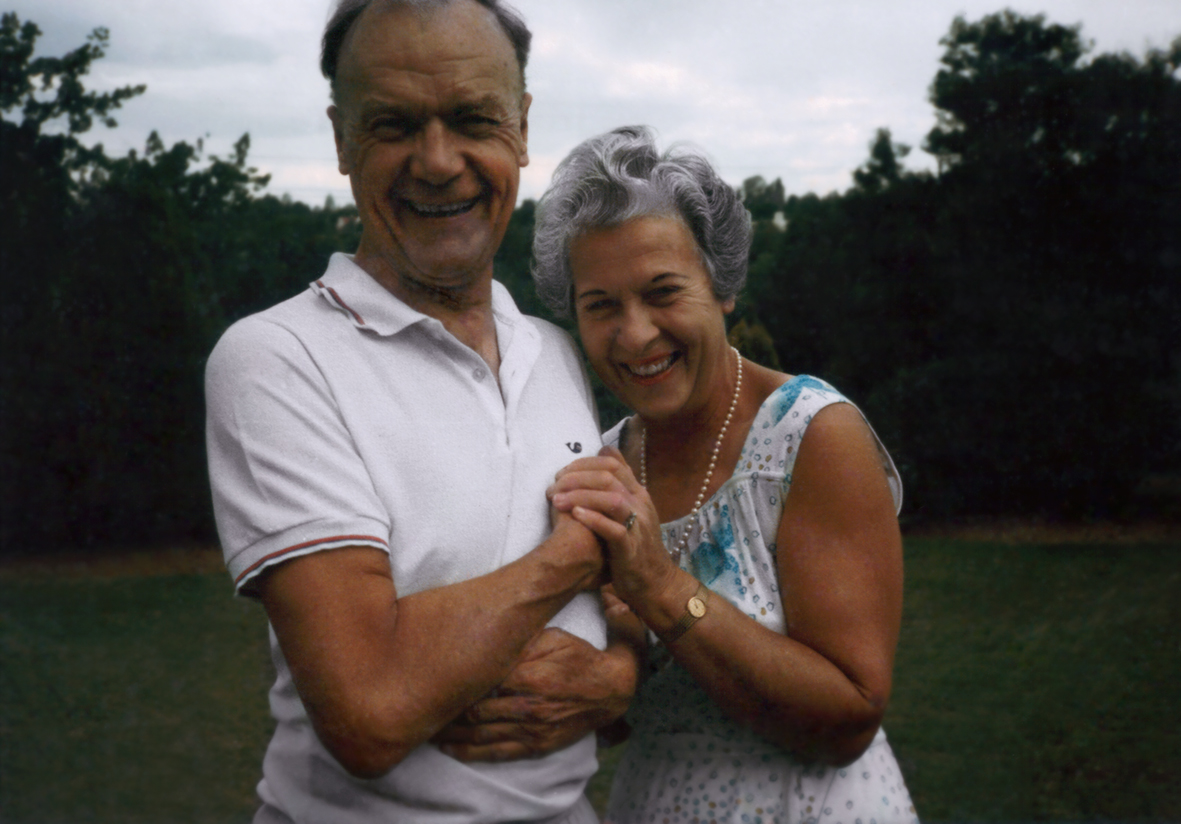
\includegraphics[width=0.45\textwidth]{photos/tony-and-madge2.jpg}\label{tony-and-madge2}}
    \\
    &
    \subfloat[Johannesburg (1982).]{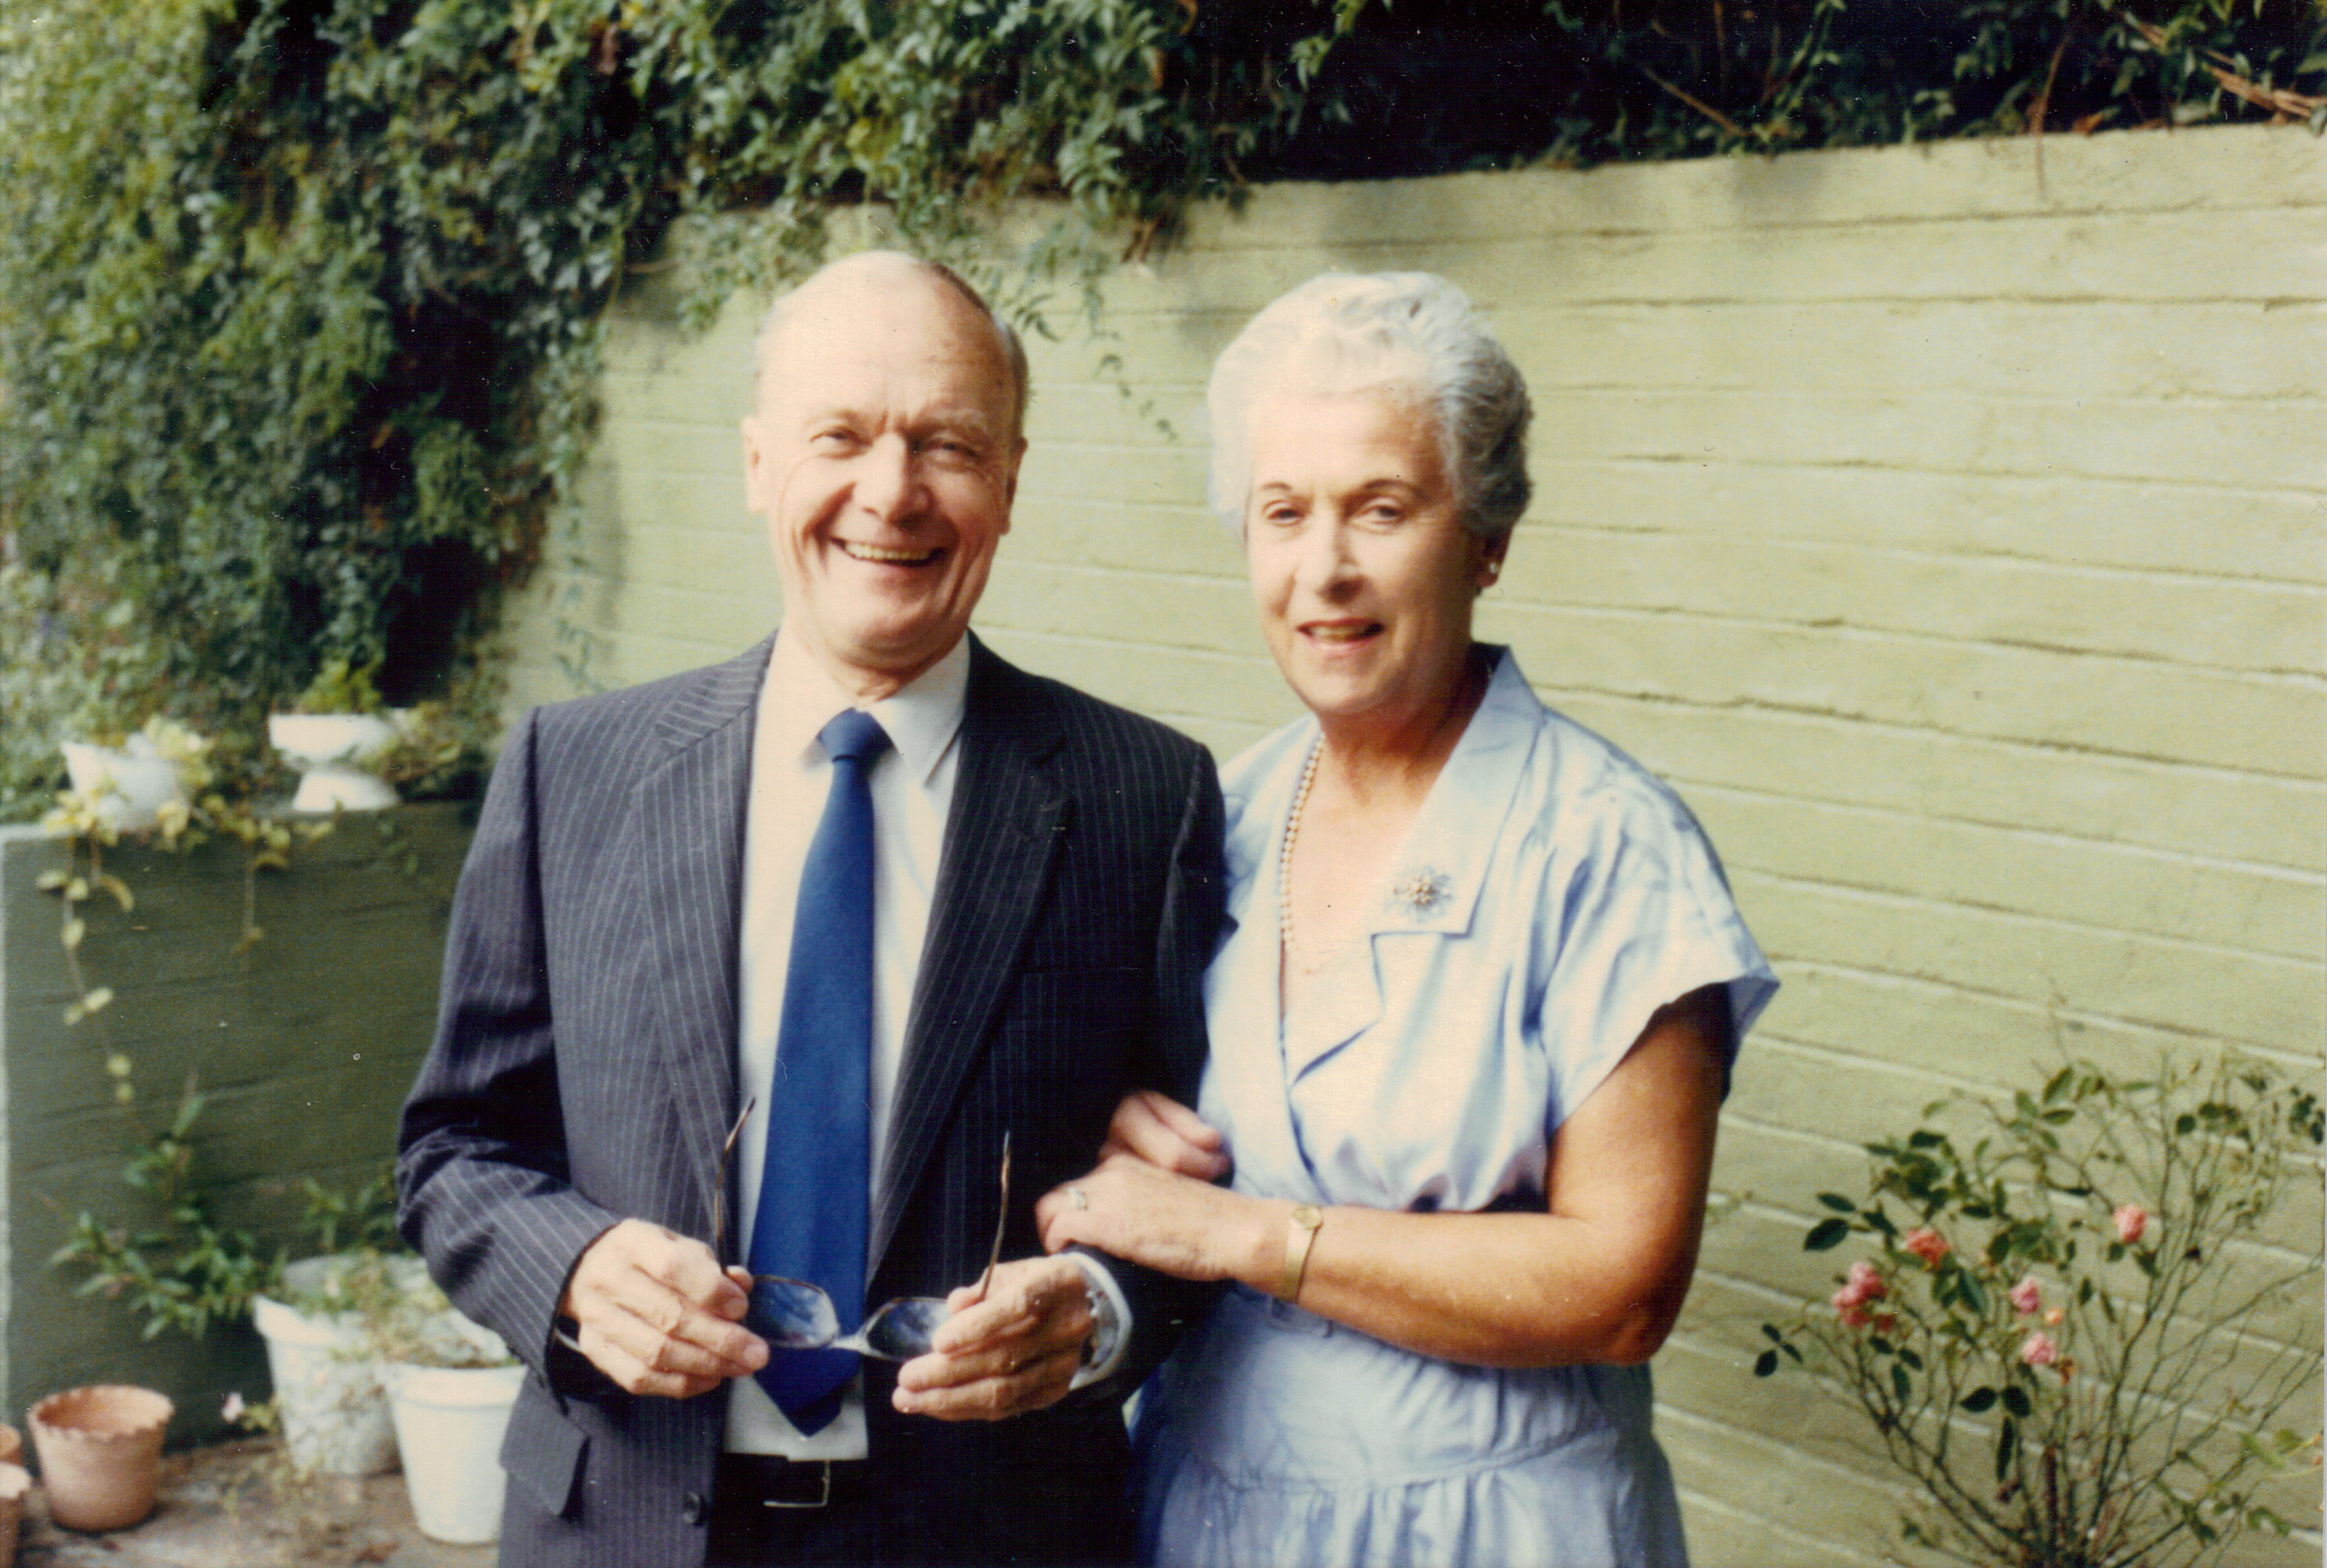
\includegraphics[width=0.45\textwidth]{photos/tony-and-madge.jpg}\label{tony-and-madge}}
    \\
  \end{tabular}
  \caption{Tony and Madge through the years.}
\end{figure}


\chapter{Turkey}

After a short while there, we flew to Turkey with a night stop in
Rome. Again we were on the Viking plane which made so much noise it
was impossible to talk! Onto Athens and Istanbul and again the train
journey overnight to Ankara.

This train (thirteen hours between Istanbul and Ankara) was to have a
lasting horrible memory for me. On a trip four years later I suffered
a miscarriage during the night and had to be ``seen to'' on
arrival. The German woman doctor was brutal and administered treatment
without an anaesthetic and Tony, poor lad, had to be with me but he
was stoic as usual. I had two more miscarriages before I produced
Elizabeth. That was after seven years. What a triumph!

There was such a lovely welcome. Tony had been there for three years
and was well-known to hoteliers, restaurant owners and staff and, of
course, the company people too.

We had to find somewhere to live but, for a short time stayed in the
Park hotel. All very strange and different.

One evening I had a panic attack! Tony had promised to take me for
dinner early and I was ready at six. I waited and waited and stood by
the window looking down on the street and realized that there was no
one who would want to talk to me and no one to whom I could talk to
not knowing enough of the language, I thought ``My mother was right, I
don't know this man, where is he?'' Tony came at 10pm having worked
until then, all was well but over the years I often wondered why it
was so impossible to pick up a telephone and tell me he would be
late. Years later in Nigeria I was waiting and the phone rang -- I
said ``Gee, I'm hungry'' and a well-bred voice said ``I'm so sorry to
hear that, Mrs. Bray.'' It was the permanent secretary to the
P~\&~T.\footnote{Post and Telegraph.} Such a nice man he never
mentioned my faux pas!

We found the time to explore Istanbul and I was enchanted with
everything there -- the cobble street, the Pera-Palace Hotel, the
Mosques and museums, the whole atmosphere was magic (the covered
market too). We often returned to Istanbul from Ankara. One evening we
went for dinner to the Park Hotel where a small orchestra played -- we
requested \textit{Amame Ecore} and always afterwards when we arrived
they would break off what they were playing and play our
tune. Romantic stuff!

Came the time to leave Istanbul for Tony had finished the work he had
to do there. He was based in Ankara and so we had to find somewhere to
live. There were several really old houses but we settled on one which
had only one serious defect -- there was a gap right across the centre
of the lounge; we learned to live with it. It could have been
dangerous but we never fell! I tried to teach Tony to dance although
he was not interested and the ``gap'' did not help so we usually
finished up laughing hysterically -- this to be followed up by some
glorious love-making!

The kitchen was primitive and so was the plumbing. Melon pips would
come down a drain right into our kitchen. Luckily we were able to
sweep the pips into another drain (I never could understand why the
two drains did not meet)!

It was dreadfully cold up on the Anatolian Plateau. We had a wood
stove in the lounge and a caretaker would come each day to clean it
out and light it. I was learning the language very slowly but enough
to take me shopping and I would practice the words of what I had to
buy as I walked down to the shops. One was not expected to pay the
prices asked but to make a pazalik (bargaining) after a while I was
brave enough to do that! I did not know it then but very many of the
Turkish people could speak English but held back. I enjoyed our little
flat but very soon I went with Tony to see other more primitive parts
of Turkey. This was an eye-opener to say the least! And I think an eye
opener too to some of the natives for I must have looked like someone
out of outer space. Turkey is a Muslim country and the women cover
their heads and faces. I was never apprehended for not covering my
head. In the winter I was dressed in slacks, overcoat, scarf and
gloves and boots -- but no hat.

The GEC telephone equipment (new, pristine and shining) would be
housed in what looked like a hovel but there were good technicians who
cared for the equipment in these repeater stations. At every town or
village Tony was greeted like a long lost cousin by these wonderful
country people and they seemed to enjoy meeting me too.

One experience I shall never forget was being invited into a small
house for morning coffee. I think that seeing me was due to
curiosity. I was set up on a dais in quite a small room where there
were no chairs or tables but pretty cushions to sit on -- half the
women of the village were there bringing babies and small
children. Everyone fitted into the room. By this time I knew enough of
the language and the questions came:

``Do you like our country?'' -- ``Yes.''

``Do you like our food?'' -- ``Yes.''

``Is England like our country'' -- ``No, it's different, but I love
Turkey.'' (tact)

``How long have you been married?'' -- ``Eighteen months!'' -- ``Then
you should have 2 children!''

It would not have been the moment to explain that one could postpone
this event so I just called on Allah and said ``Allah versin'' (Allah
will give) or ``Inshallah'' (Allah will know the moment). Phew!  This
was accepted. We had delightful sweetreats and Turkish coffee. I felt
very pleased and proud of my ``press conference''!

Staying in a village ``hotel'' was something else. There was but one
wash basin for the entire complement of visitors. And I had to queue
up with other ``guests'' (mostly men) to wash my face and hands
only. My mother would have been horrified but nothing was going to
daunt me then. Tony would not have wanted a grizzling wife!

It was a relief to reach another hotel sometimes and to have a welcome
bath. One place we stayed in was built of cow manure and
whitewashed. Snakes could come out of the ceiling but I never saw
one. Oh! We had to ask for clean sheets for they were seldom
changed. What a paradise to return to Ankara or Istanbul and savour
the clean cool sheets!

There were lovely things to have on these trips and I will never
forget the huge peaches of Bursa or the melons of Diyarbakir. This
latter place was surrounded by a thick, thick wall where there were
thousands of scorpions -- school children would collect them and bring
them, dead or alive and be paid handsomely for each one. Hospitality,
scenery and sunsets played a large part in these travels and one
always remembers the nice aspects.

It was nice to return to our funny little flat but often for a short
time for our travels would begin again and Tony would have more
installation work to do. It was good to get away sometimes from the
hopelessly crippled beggars who would come knocking at the door. It
was common practice for babies to be maimed at birth in order to be
able to spend their lives begging. I am ashamed that I would just slam
the door but it was often a very awful sight.

Once whilst I was waiting for Tony in some public place in Istanbul, I
was sitting opposite a man who kept staring at me. The Turks are known
for this habit but I objected and poked my tongue out at him. Tony was
furious -- I could have got a knife in my back!

The time came for Tony's contract in Turkey to finish and we had a
final tour to Istanbul and Izmir (Smyrna in the Bible) this was
intensely interesting because we had the opportunity to go to Ephesus
(Efus in the Bible) from Izmir. There is too much history to be told
here. It is a always wonderful experience to stand still in historical
and ancient surroundings and think of the amount of history which has
taken place there. Several of St. Paul’s journeys were made in Turkey
and it is daunting to realise that the very ground one is standing on
is still the same as it was centuries before. How lucky I am to have
seen all of this and how lucky to be able to remember it. Goodbye
Turkey -- I shall never forget you!


\chapter{Elizabeth \& Richard}

Even before she was born, Elizabeth showed a tenacity and strength of
purpose. For, in spite of a set back at Christmas~1959, she hung on
and was determined to be born which indeed she was in July~1960. She
was a beautiful and contented child and we delighted in her.

There is always another Mother Grundy lurking -- someone who likes to
bring criticism and unhappiness into another person's life. I met such
a person when I was out pushing Elizabeth in her pram. She said ``That
child is sucking her thumb because she lacks something in her life --
probably love''. To which I replied ``Madam, we have waited 7~years
for this child and she lacks nothing, least of all love, except
perhaps a carpet in her bedroom and I am quite sure she is unaware of
that.''

% We had arrived back from Turkey in 1956 and were quite settled into
% our lovely house in Leamington Spa when Tony was offered a top posting
% with the GEC in Nigeria.

We had arrived back from Turkey in 1956. Returning to England from
Turkey was very different and the five years we spent there had their
difficulties. Tony had ``almost'' a gastric ulcer according to the
doctor. He did not settle down to factory life and felt inhibited by
the set hours. He had been used to travelling long distance and having
quite an adventurous way of life.

We built a house in Leamington Spa close to the GEC in Coventry. We
bought new furniture and developed the garden (well I did). It was a
useful time for this when Tony went off to Finland for two business
trips -- one of three months and one of ten weeks. I took off the turf
and then dug deep and grew marvelous vegetables (and raspberries and
almost killed Tony with the acid). Nothing to it. Of course the ground
had been a horse paddock and so was very well manured.

All this exercise had to stop when I became pregnant with Elizabeth. I
had to be extra careful as I had had two miscarriages. She arrived in
July 1960. No one but me had ever had a baby! We had had to wait for
seven years.

We were quite settled into our lovely house in Leamington Spa when
Tony was offered a top posting with the GEC in Nigeria.

He had to undergo certain tests and the doctor who pronounced him fit
said ``I have bad news for you, old chap -- you will be able to go to
Nigeria.'' We both had to have injections for typhoid, TB, yellow
fever, etc. Our house had to be sold and the furniture put into
storage; I was so upset that I could not watch the removal van drive
away.

Tony flew on ahead to Lagos but Elizabeth and I made the 13~day trip
by sea. My dad drove us and the 2 grandmothers to Liverpool to embark
on the ship.

They were heartbroken at the thought of our being taken to that
``God-forsaken place'' and I could not help feeling sorry for
them. Tony's father had passed away and never saw his
granddaughter. He would have been terribly upset by this parting.

March is not the best time of the year for crossing the Bay of Biscay
for the sea is very turbulent. So much so that I succumbed to
sea-sickness and felt very ill for 5~days.

Once more, Elizabeth displayed her stoicism by marching up the deck as
if in a straight line. I had to carry on; she loved her food and I had
to carry her up 2~flights of stairs to the childrens' restaurant --
hopefully finding a place for her by the door so that I could exit
quickly to the bathroom!

Once we had passed the Canary Islands I felt much better and was able
to enjoy the wonderful food and activities. One can understand the
temptation of shipboard romances. The whole atmosphere was wonderful
-- the incredible inky blue of the sea in the moonlight, the smooth
passage of the ship through the water after the awful turmoil, and the
constant playing of ``Moonriver'' over the sound system. I shall
always love that song (as I write this in September 2012, I hear that
Andy Williams, the composer, died yesterday; what a lovely song and
tune he left).

Apparently I ``waddled'' off the ship due to the good food. It was
great to see Tony again but oh! arriving in Lagos was like walking
into hot pea soup with the temperature and humidity at impossible
levels.

Never mind -- we were a family again.

Once we were accustomed to the climate, life became reasonably
enjoyable. For the 11~years we were in Nigeria we occupied the same
house; even when we went on leave, the house was always
``ours''. There was air-conditioning upstairs but we had to lose the
comfort of this many times due to the frequent electricity cuts --
sometimes up to 72~hours. Nigeria had gained independence in 1960 and,
inevitably, basic services failed.

Our house was one of 4 in a compound and in the grounds were the
servants quarters. In one of these lived a little black girl. She and
Elizabeth became good friends and they played together in our garden.

When she was 4, Elizabeth started attending St. Saviour's school. This
was a Church of England school attached to St. Saviour's church in
Lagos where the rector was Reverend Jim Payne; his wife, Dorothy Payne
was the headmistress of the little school.

All the teachers were expatriates and it was interesting to see pupils
of different nationalities attending the school. But the majority were
Nigerian because the government only allowed the school to function if
this were the case.

A mixture would turn up at one of the birthday parties and once, there
were 5~Nigerians. When I remarked on this, Elizabeth said ``Does it
matter?'' Of course not. Children do not notice colour.

Our house boy, Audu, from the northern Hausa tribe, was as efficient
in the garden as he was in the house. He and Elizabeth developed a
strong friendship. One day she brought home from school a ``Flame of
the Forest'' seed. Audu planted it in a tin and nurtured it until it
was ready to plant in the garden. It grew well and, eventually,
reached the height of the balcony. Unfortunately, a parasite plant had
wound itself around the tree. Before leaving for work one day Tony
said to our gardener -- Andrew -- ``Get that thing down,'' meaning the
parasite -- and he did, tree and all.

Audu and I were in a state when she came home from school. She cried a
lot (so did I) but she squared her shoulders and dried her tears and
said ``Well I must try again,'' which she did with Audu's help and
actually that tree grew taller and stronger than the first one (see
Pictures~\ref{elizabeth-with-audu} and \ref{elizabeth-with-gardener})!

In 1964 we granted Elizabeth's wish for a baby brother and Richard was
born. Because of a bad history I went back to my home town for the
birth, much to the disappointment of one Dr. Ogan in Lagos who tried
to persuade me to stay. He was such a nice man; he loved London and
the English people and also Australia and, only in the last 5~minutes
of the conversation, he would say ``I suppose we'd better take a look
at this baby.''

Elizabeth and I stayed with my parents in Anton and because of Tony's
stop-start attempts at getting some leave, we did not return to Lagos
until Richard was 6~months old (see Pictures~\ref{tony-family}).

% \begin{figure}
%   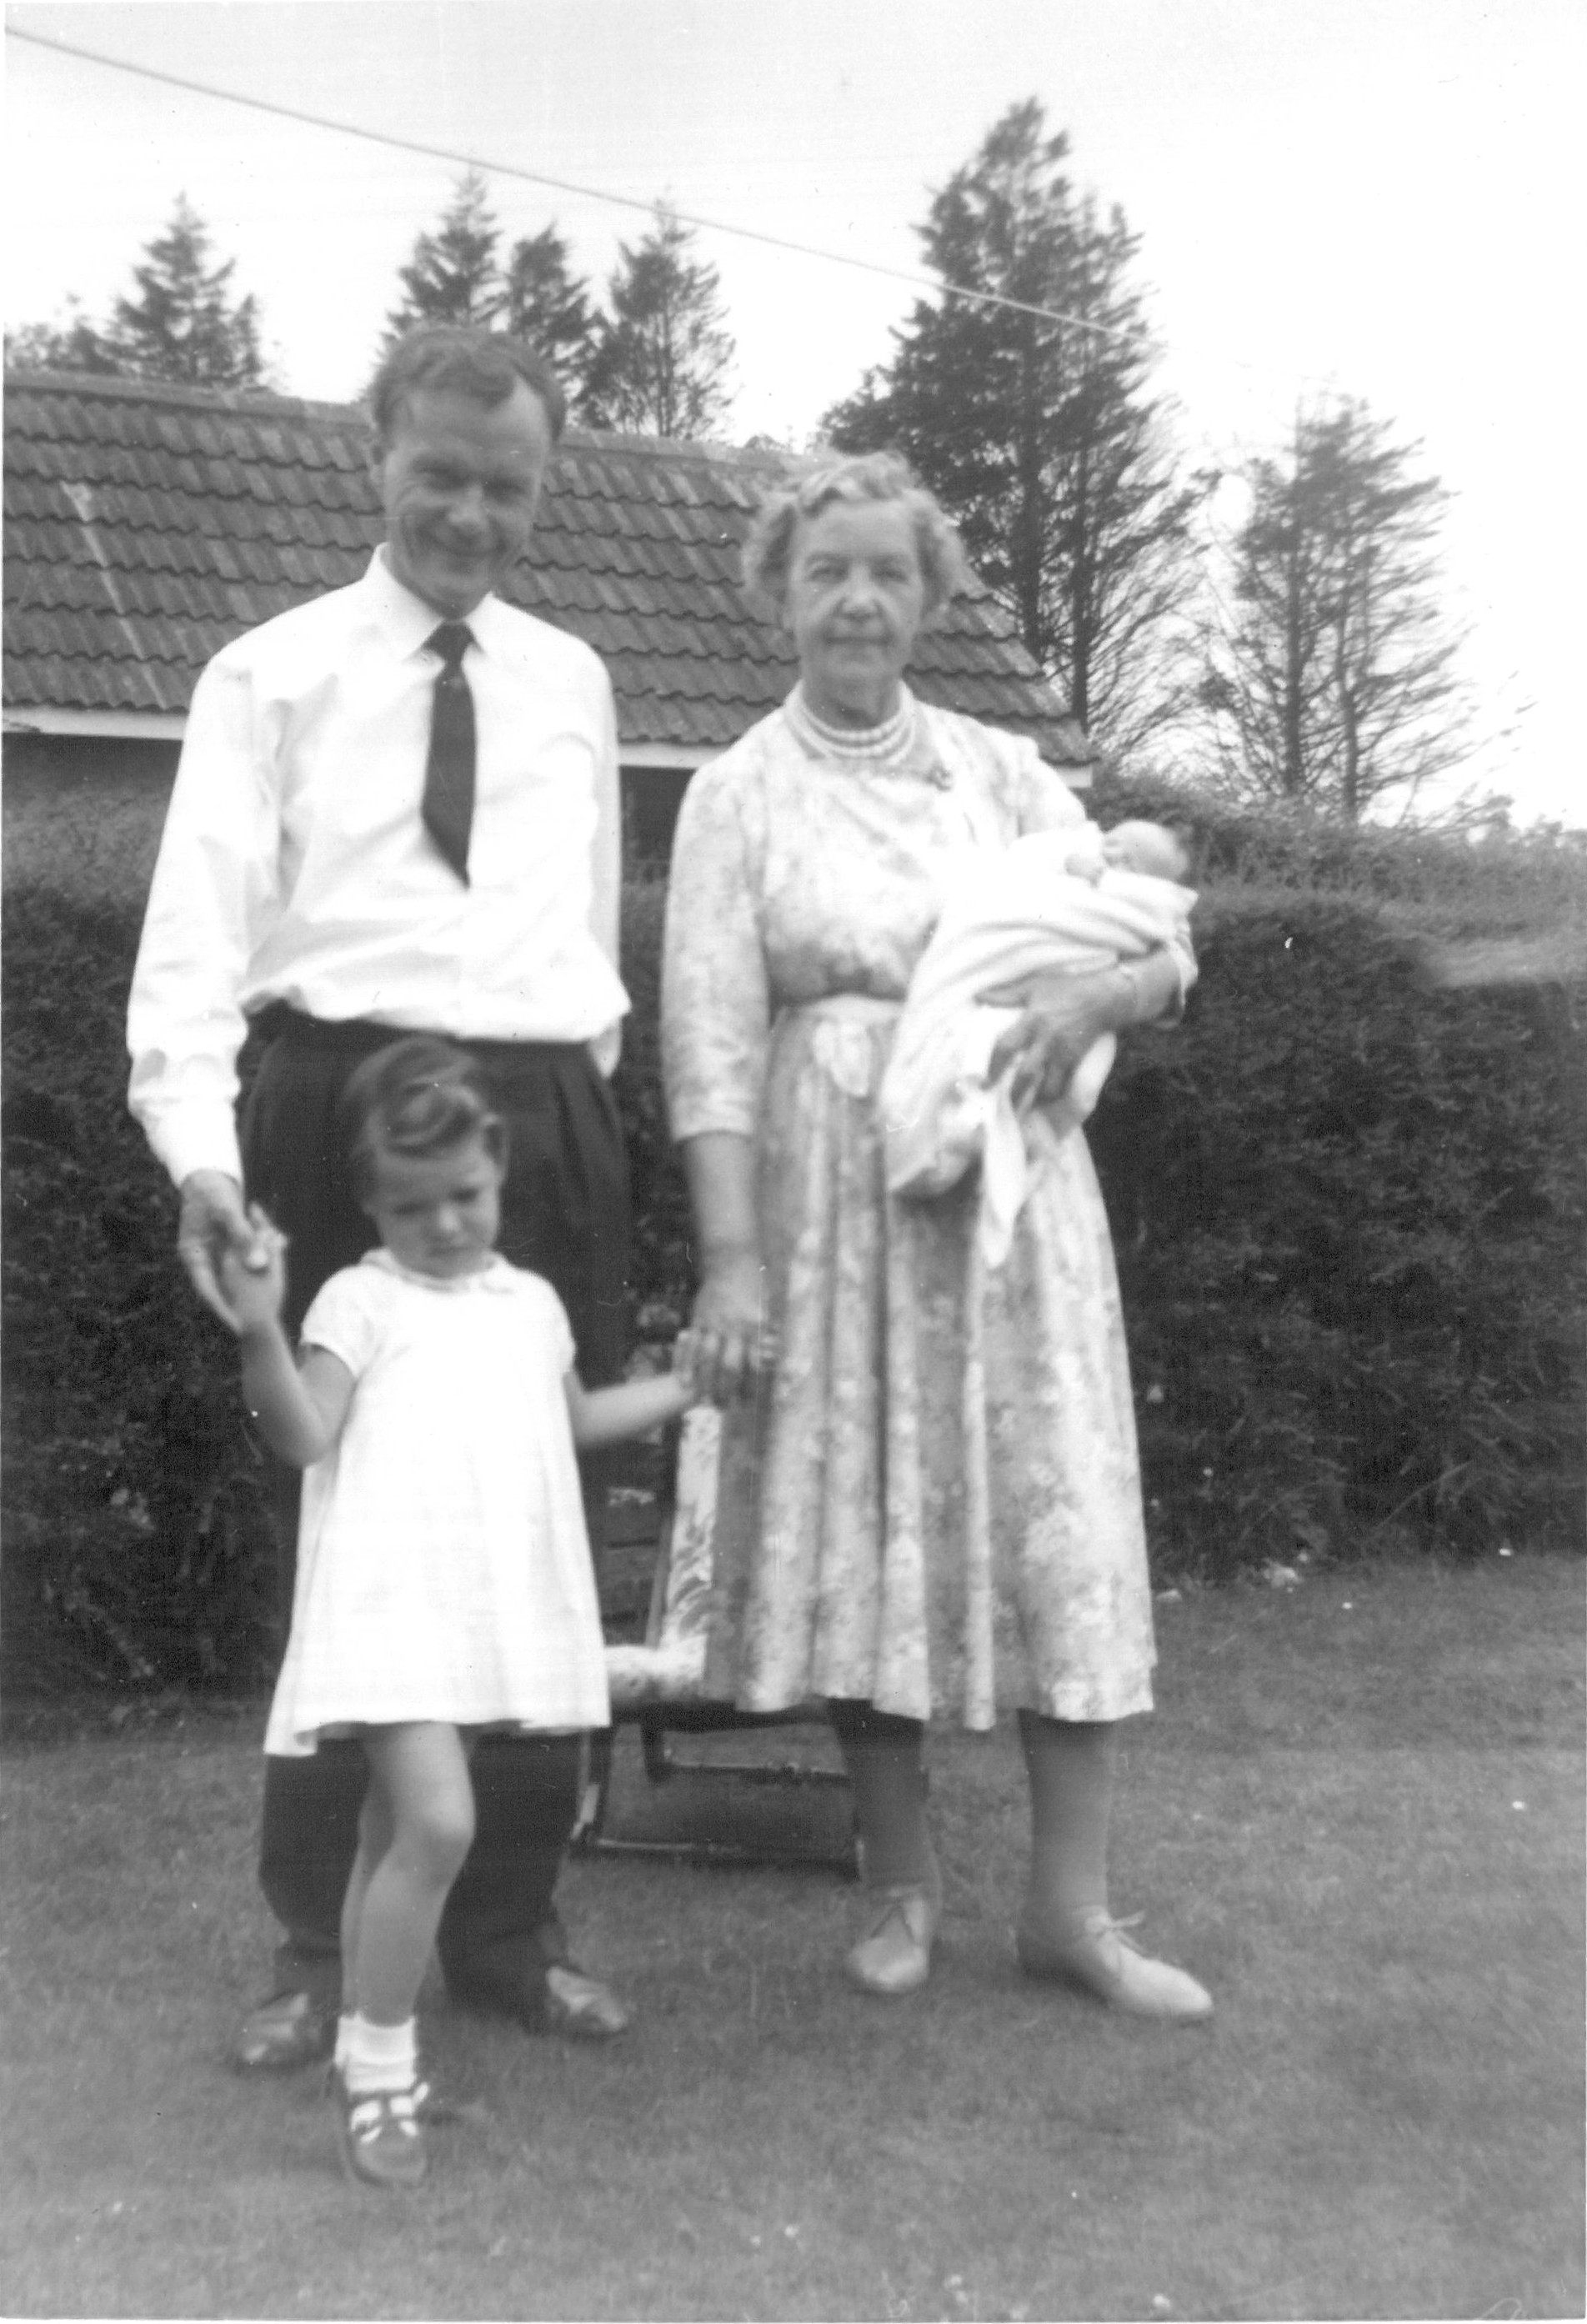
\includegraphics[width=\textwidth]{photos/tony-with-mother}
%   \caption{Tony with his mother, Elizabeth, and Richard (England, 1964).}
%   \label{tony-with-mother}
% \end{figure}

% \begin{figure}
%   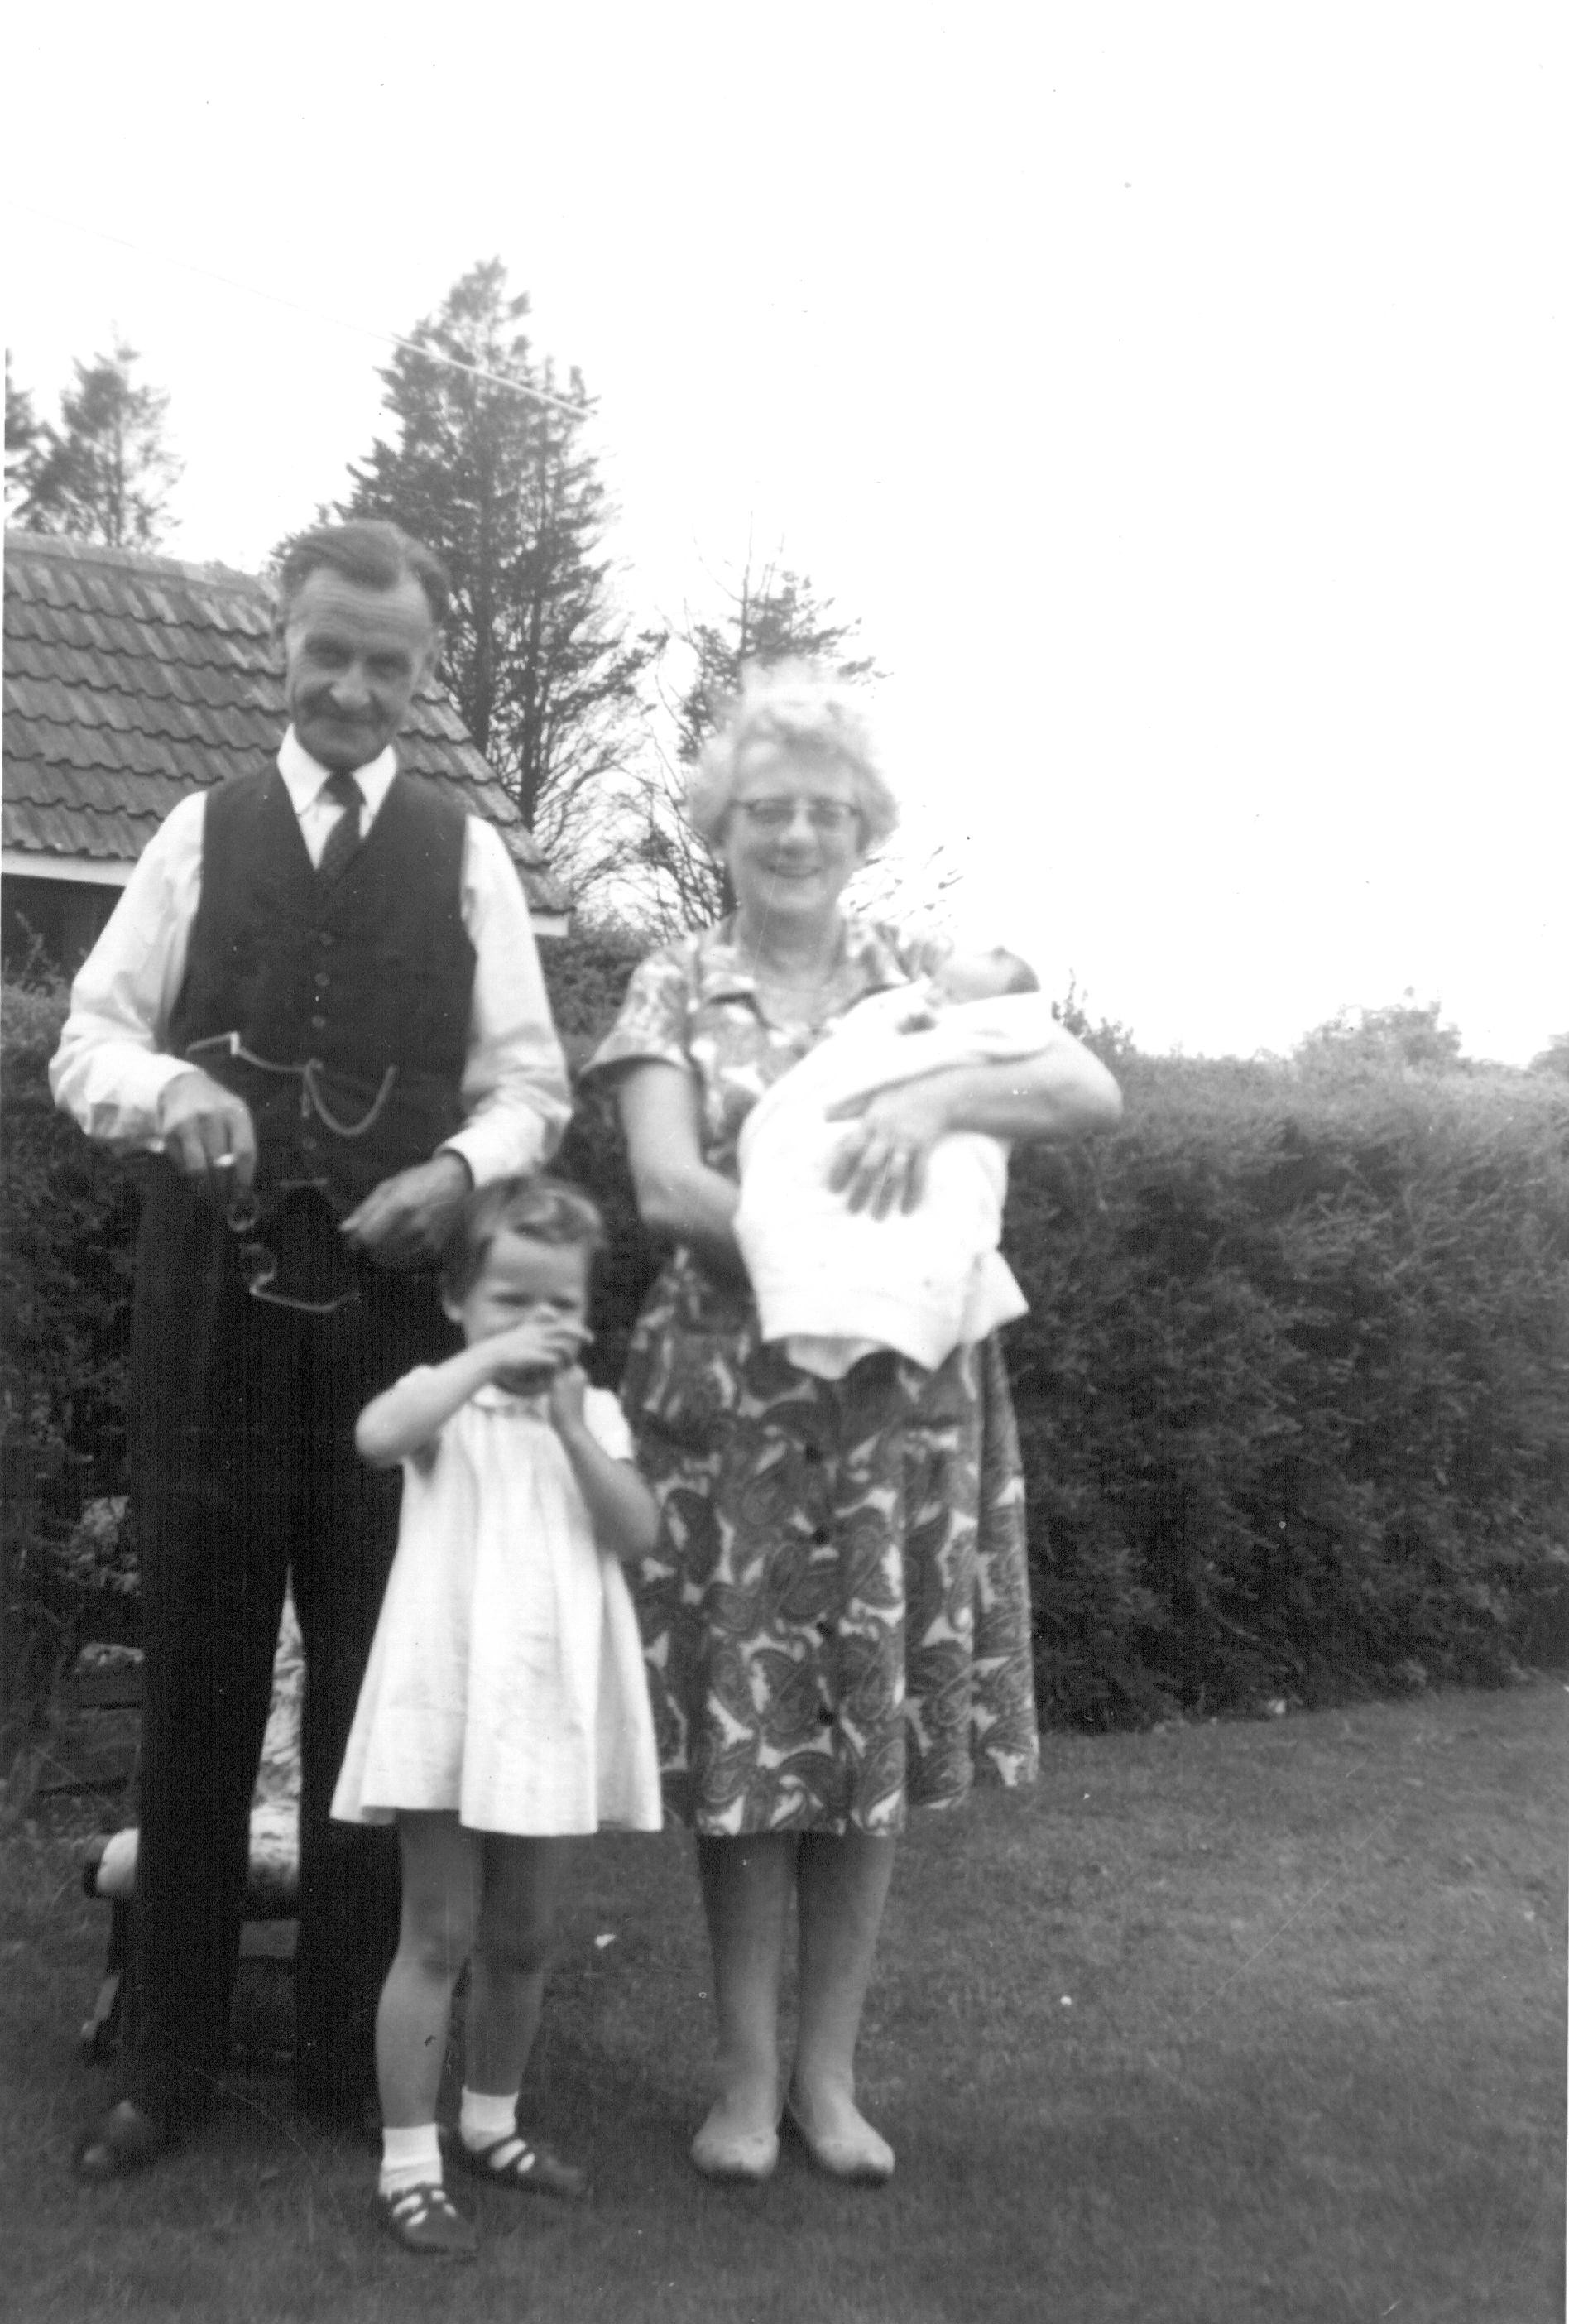
\includegraphics[width=0.9\textwidth]{photos/tony-parents}
%   \caption{Tony's mother and father with Elizabeth and Richard
%     (England, 1964).}
%   \label{tony-parents}
% \end{figure}

\begin{figure}
  \centering
  \begin{tabular}{cc}
    \subfloat[Madge's mother and father with Elizabeth and Richard.]{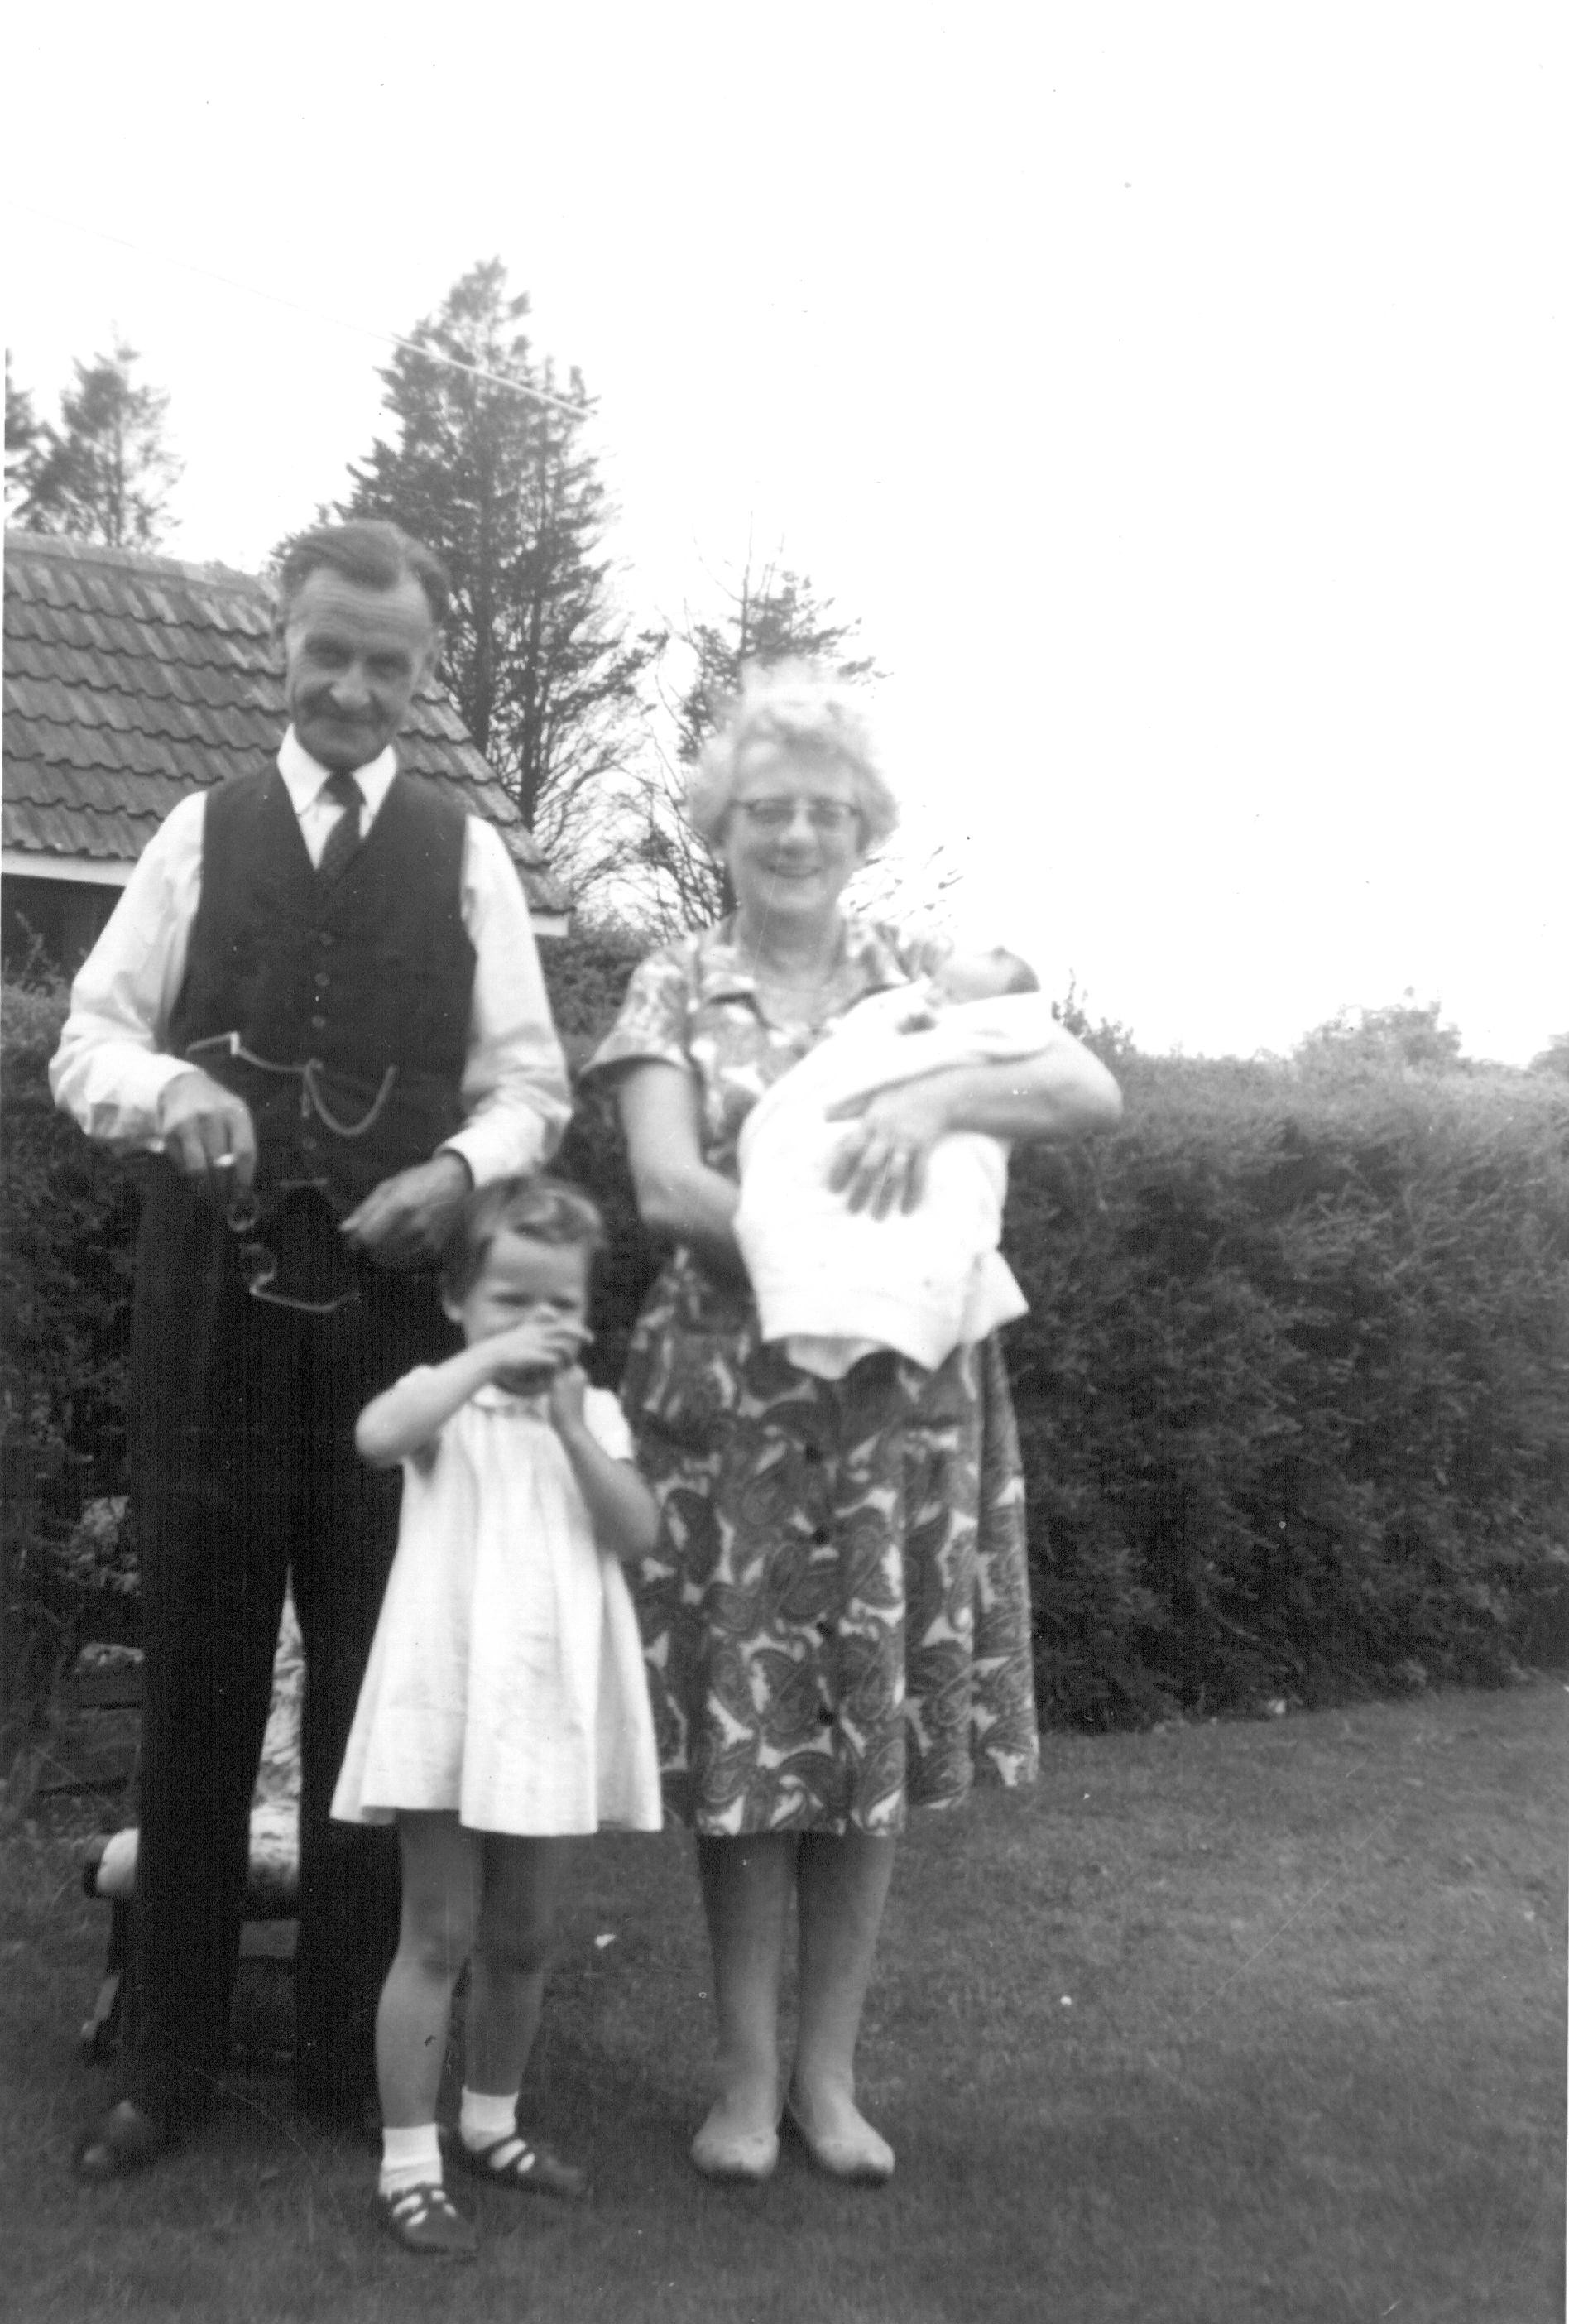
\includegraphics[width=0.45\textwidth]{photos/tony-parents.jpg}\label{tony-parents}}
    &
    \subfloat[Tony with his mother, Elizabeth, and Richard.]{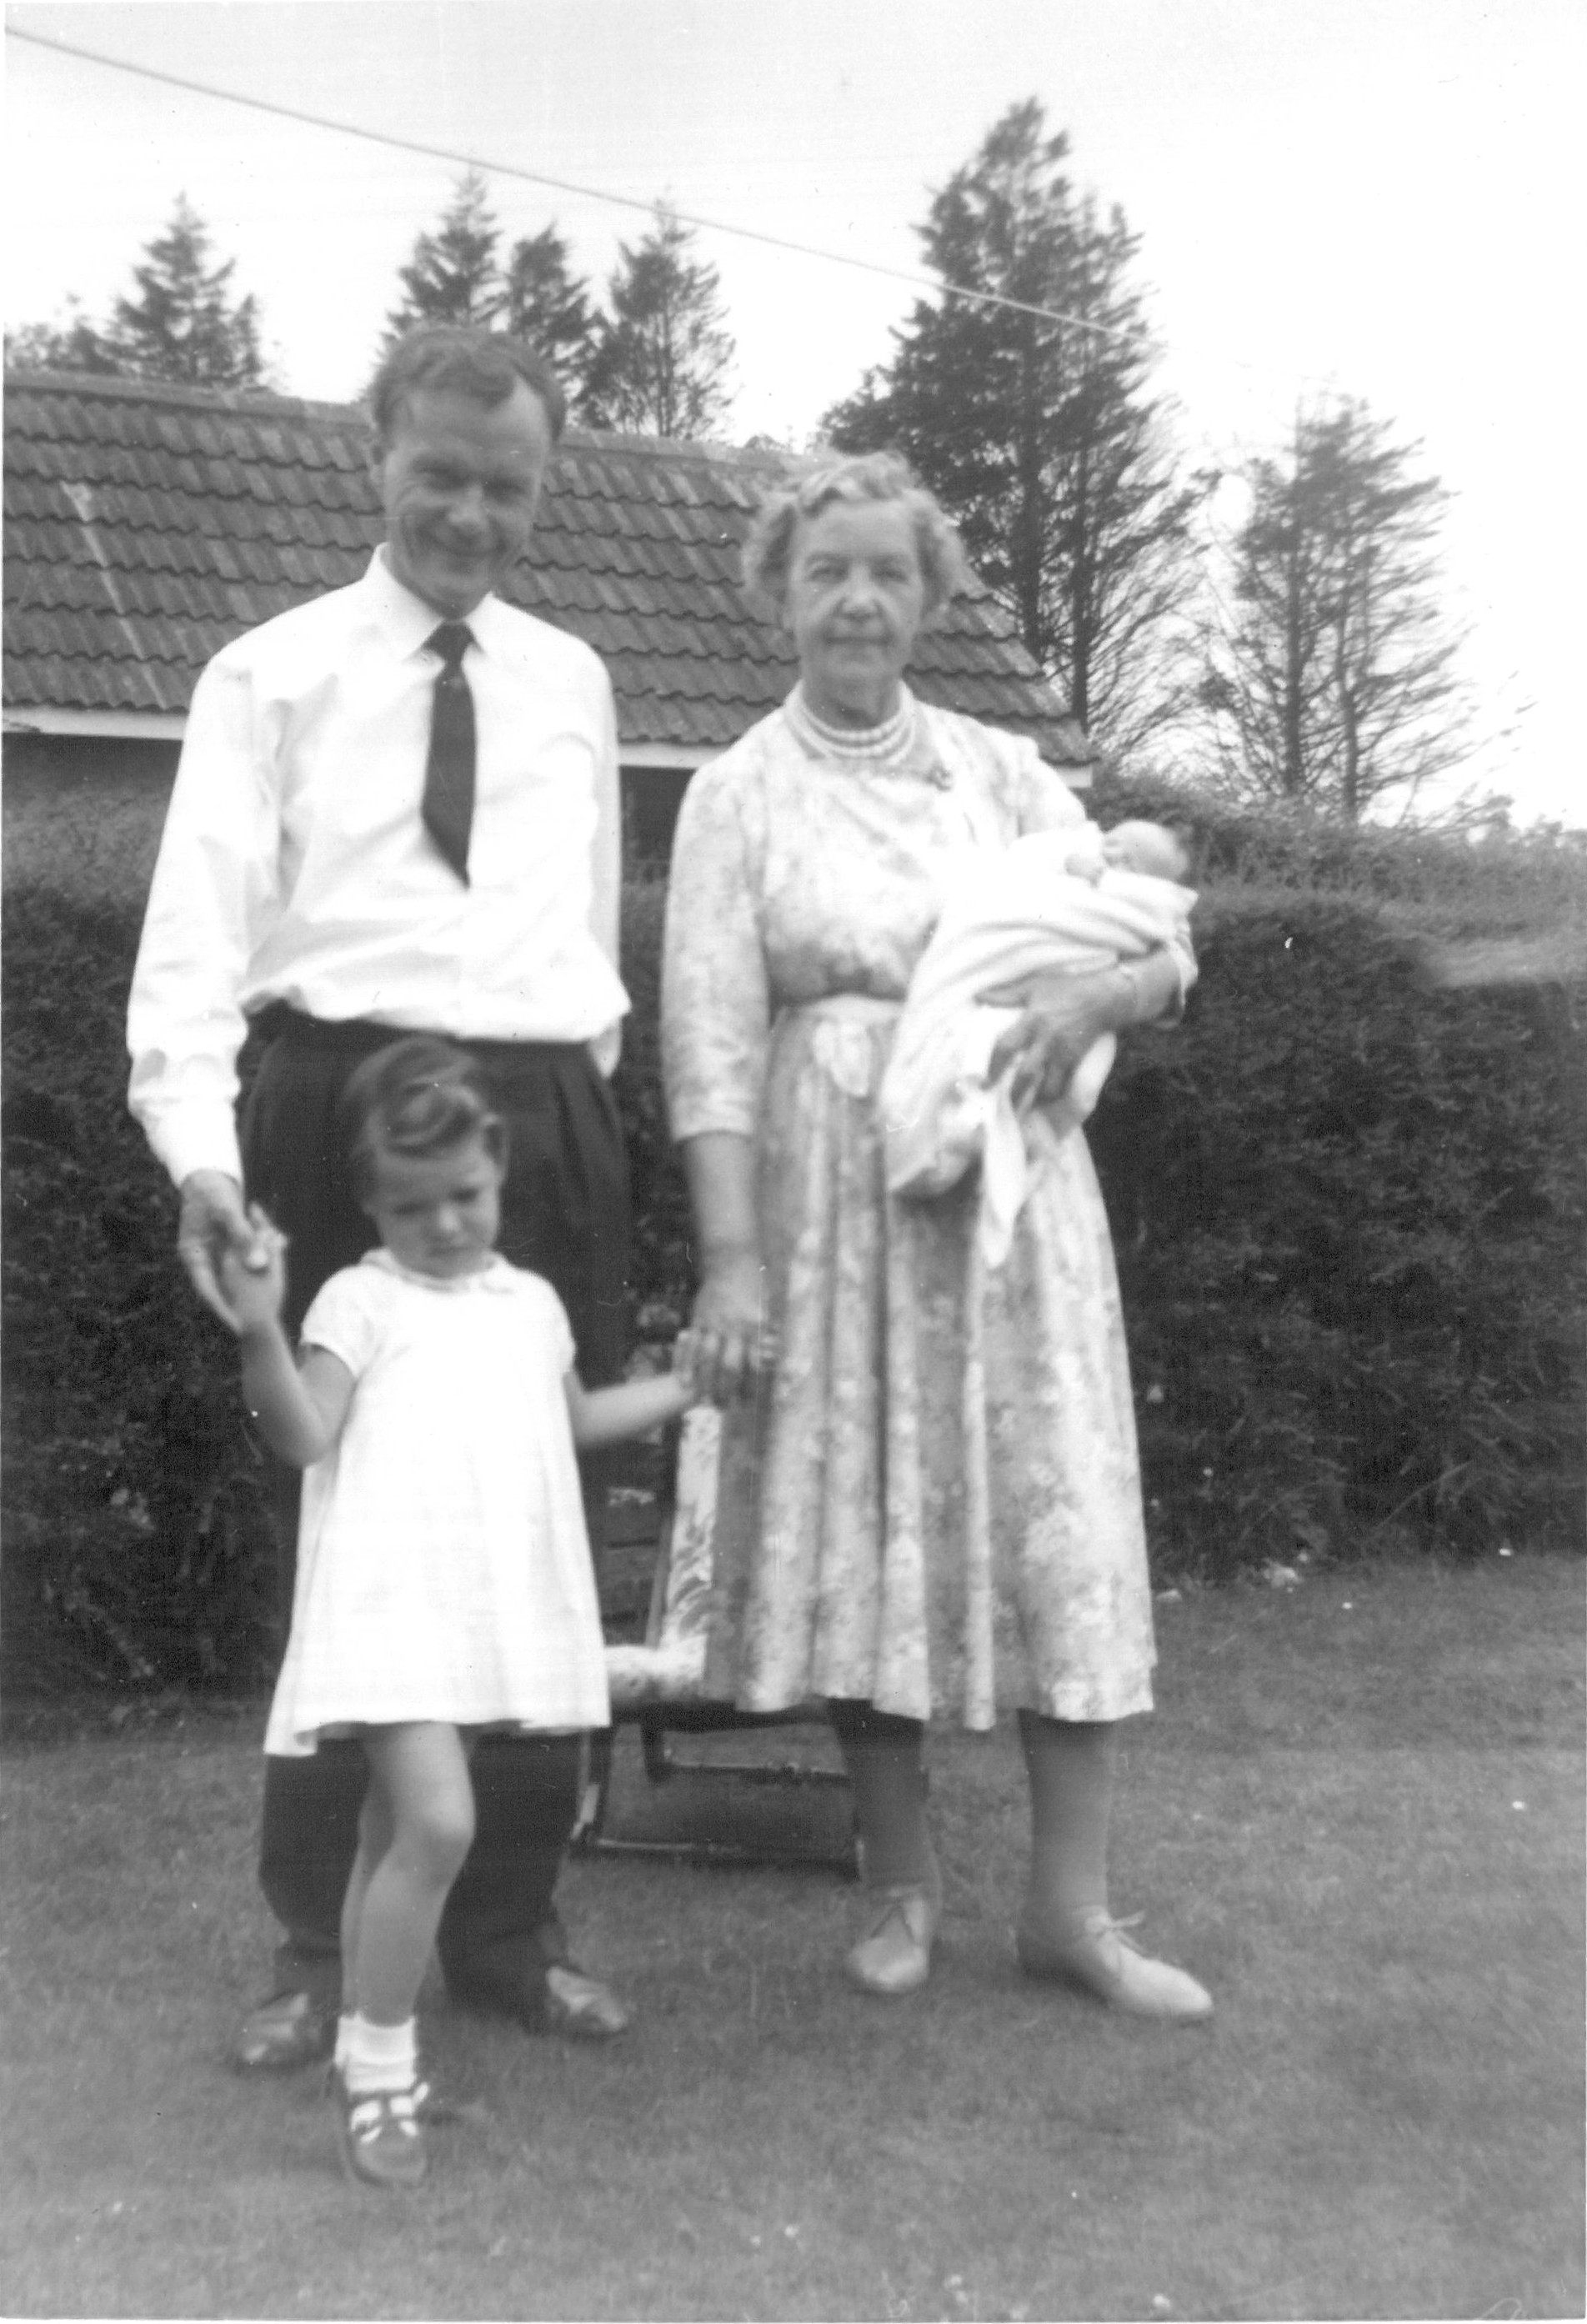
\includegraphics[width=0.45\textwidth]{photos/tony-with-mother.jpg}\label{tony-with-mother}}
    \\
  \end{tabular}
  \caption{Family (England, 1964).}
  \label{tony-family}
\end{figure}


Elizabeth became the ``Little mother.'' We had some laughs; a changed
nappy would finish up round his ankles and the lime juice once given
to him caused him serious problems.

When Richard was 4, he started going to St. Saviour's school and was
lucky to have Elizabeth there to keep an eye on him. He and Elizabeth
both enjoyed the school which was a very happy place (see
Picture~\ref{young-children}).

% \begin{figure}
%   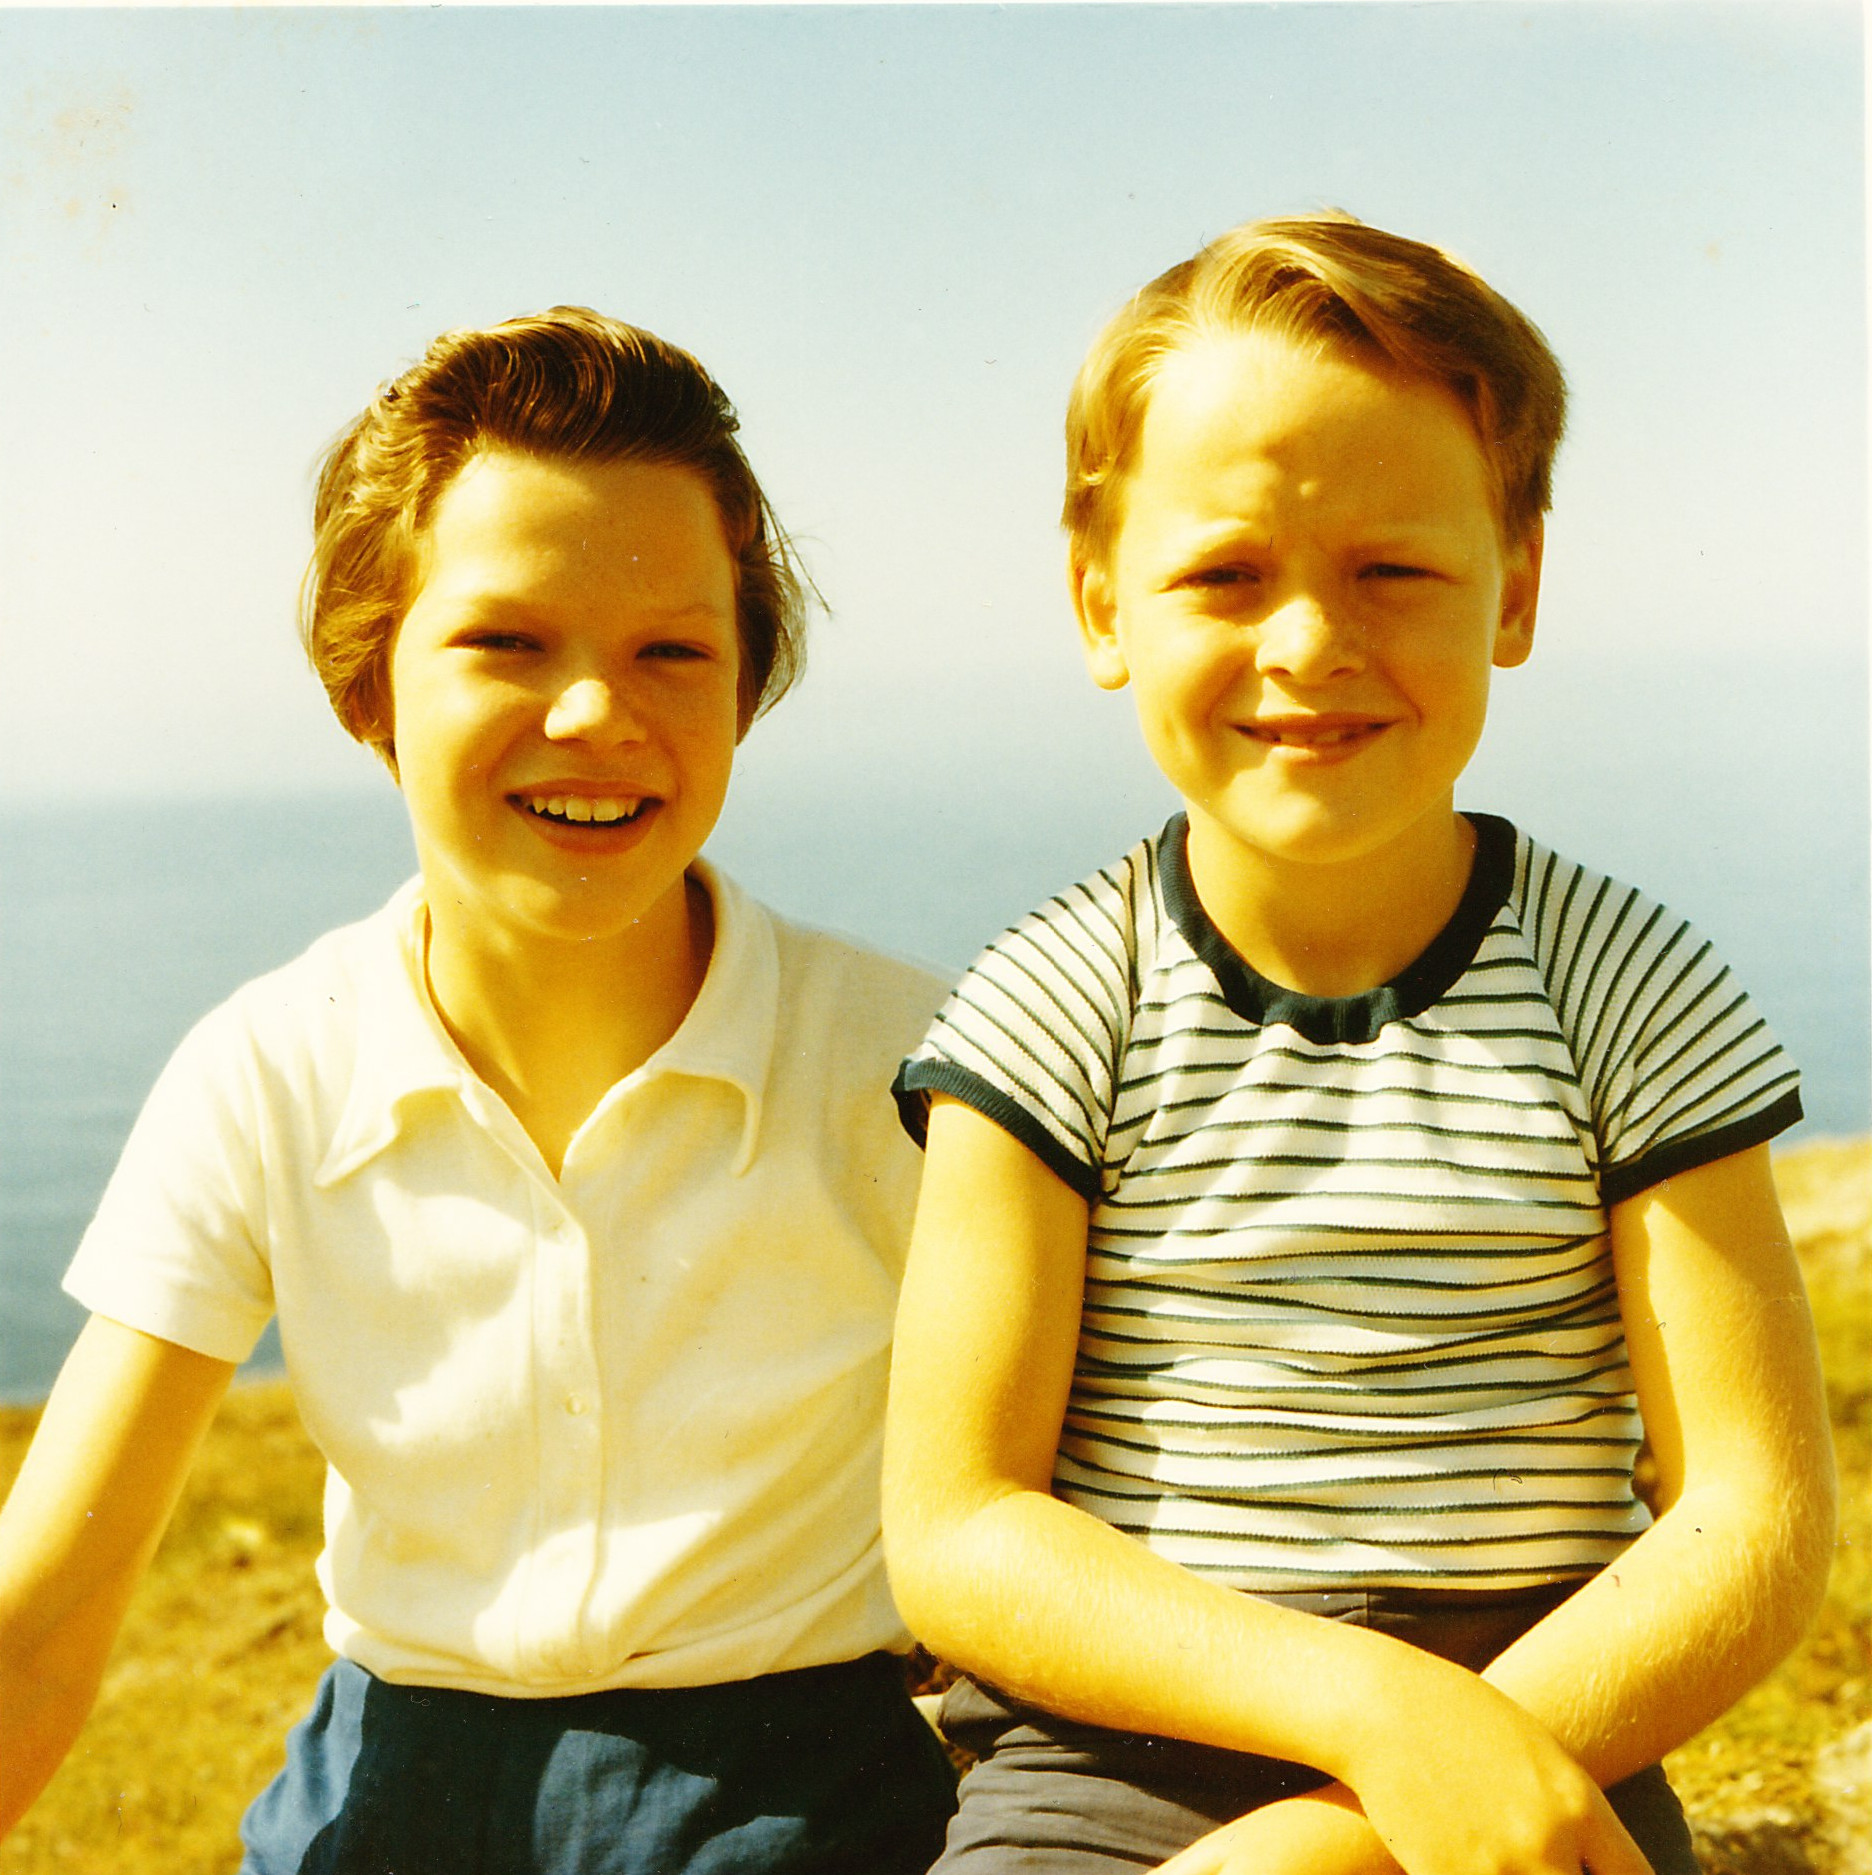
\includegraphics[width=\textwidth]{photos/elizabeth-and-richard}
%   \caption{Elizabeth and Richard.}
%   \label{young-children}
% \end{figure}

We warded off the dreaded malaria by taking regular
medication. Cholera became endemic while we were there and we had to
be more particular than ever about filtering and boiling the water.

And we were especially careful about the various diseases caused by
the parasites entering the body. The children often went into the
garden dressed only in pants and a light shirt but \textit{always}
shoes and socks because some of these delightful creatures would enter
through the feet.

Life continued happily until Elizabeth was 11 when, because there was
no further schooling for ex-patriot whites, we had to send her to a
boarding school in England. We chose Wroxall Abbey in Warwickshire and
she was reasonably happy there. The company (GEC) paid her holiday
fares to see us and she became a calm and seasoned traveller.

Richard continued at St.~Saviour's until he was 7 and then we moved to
South Africa and we were all together again.

We settled in Johannesburg (see Picture~\ref{bray-family}).

\begin{figure}
  \centering
  \begin{tabular}{c}
    \subfloat[Elizabeth \& Richard (1969).]{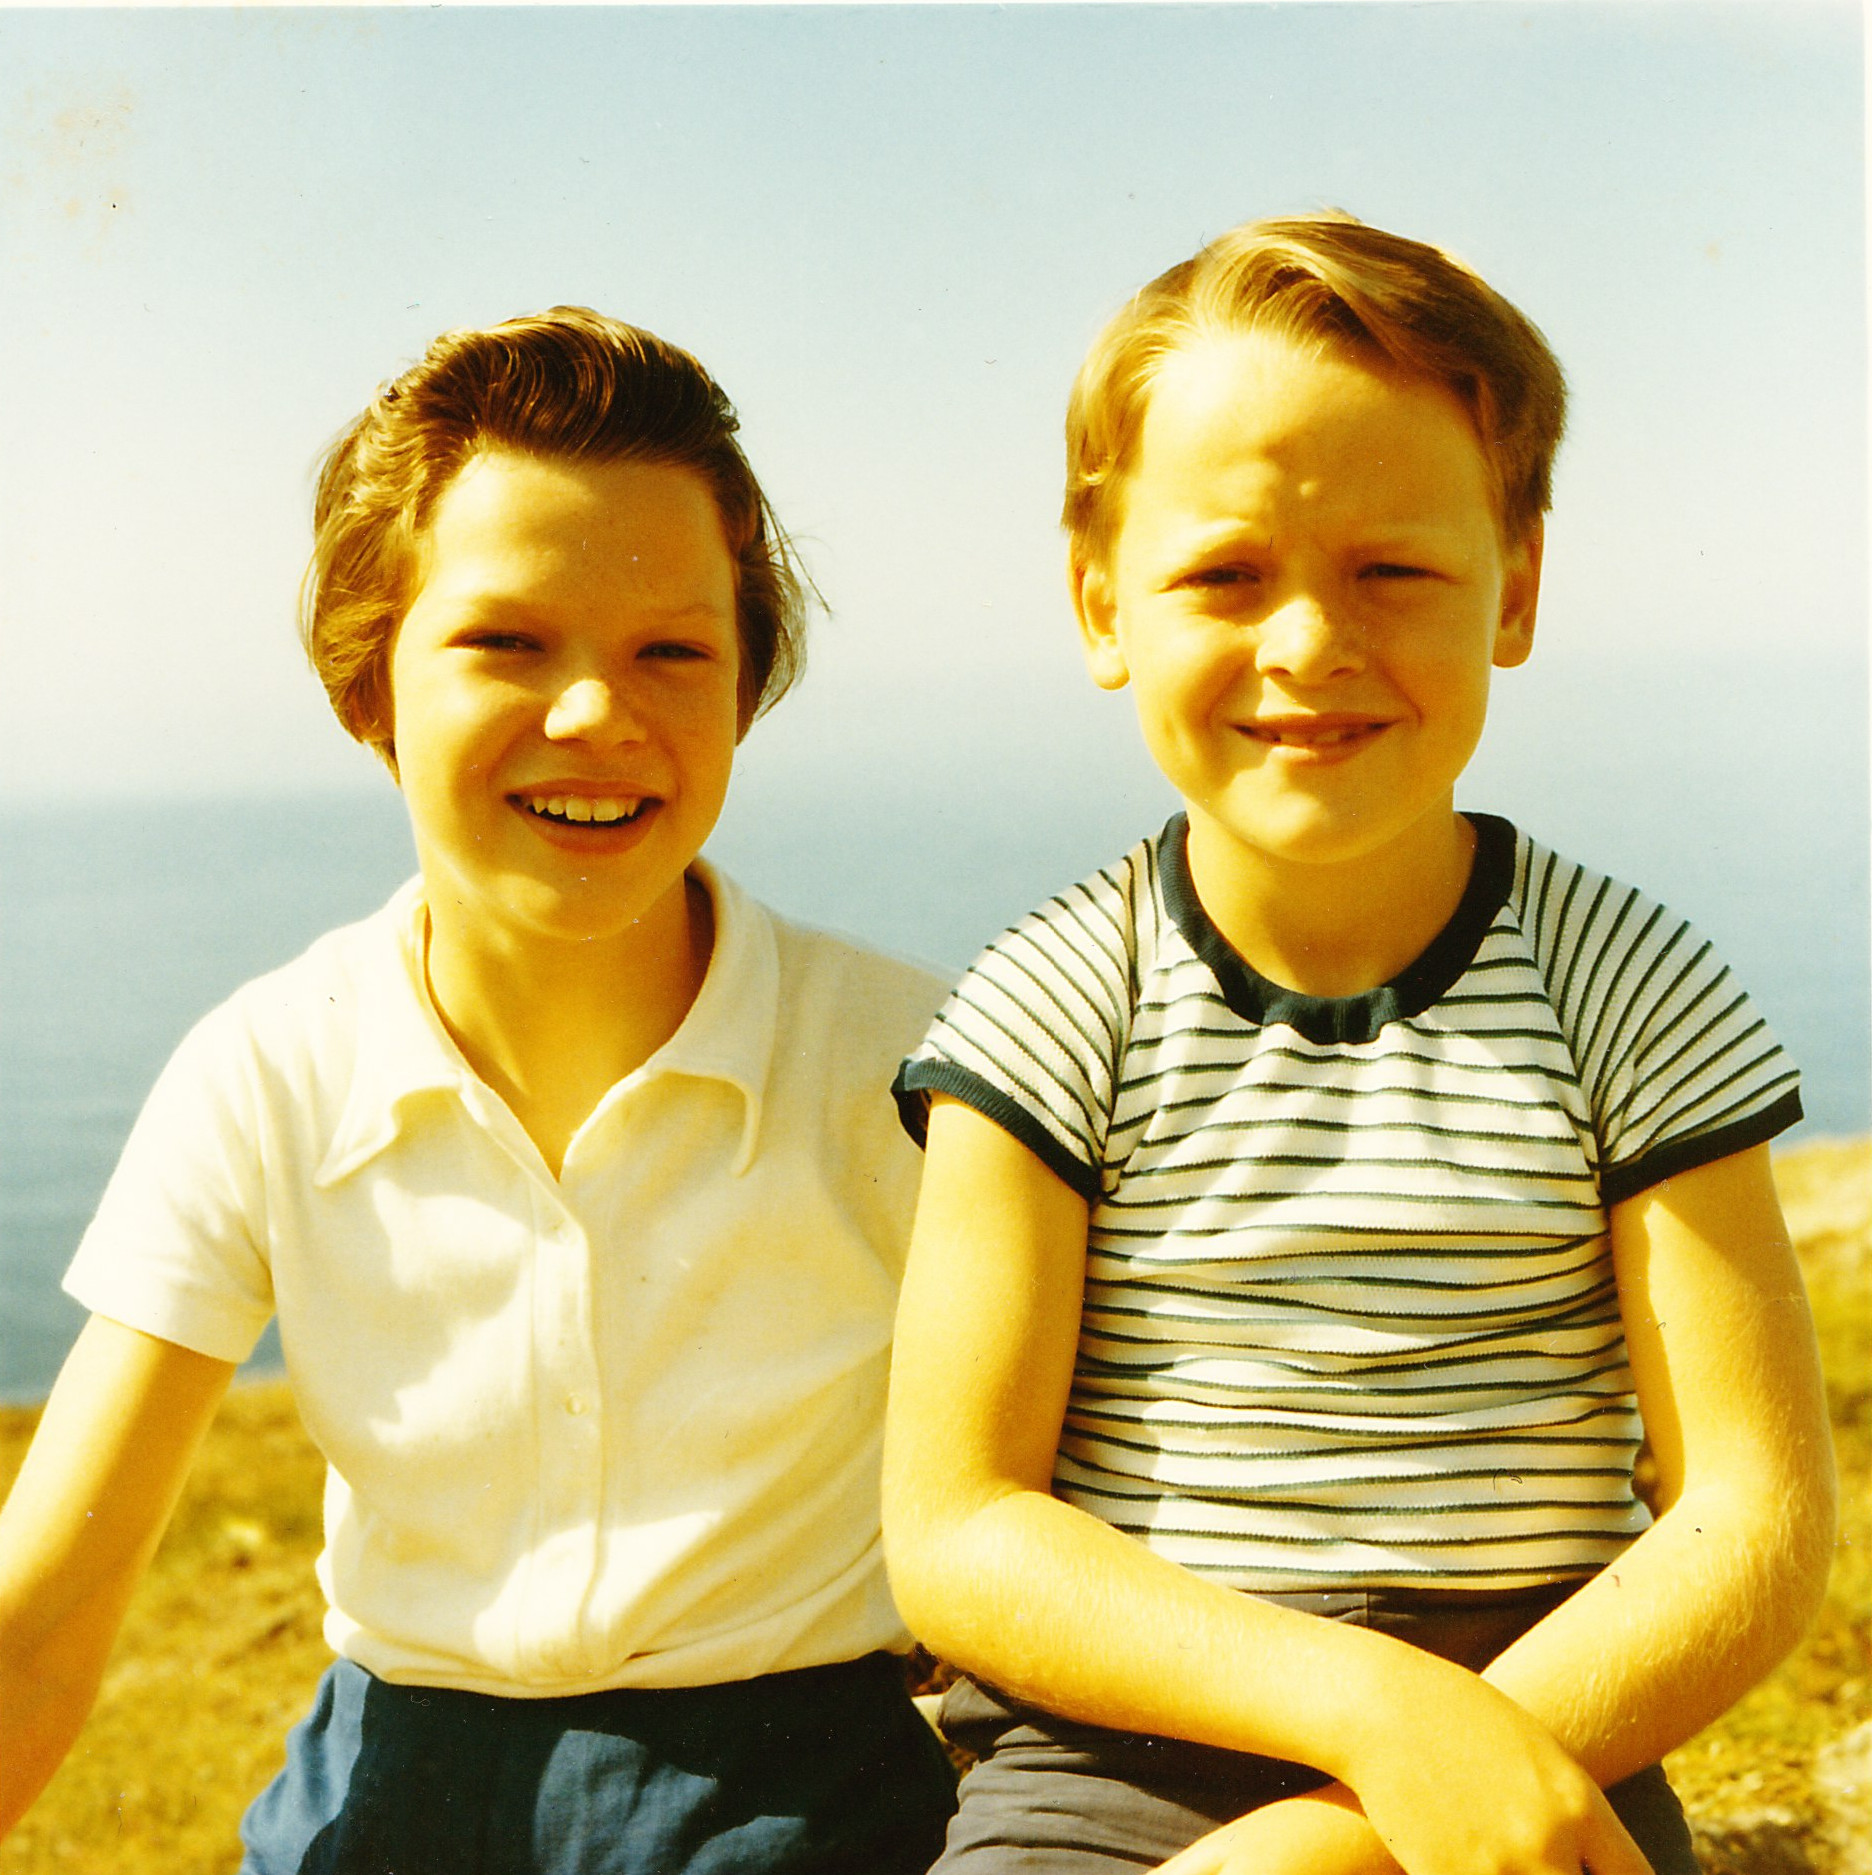
\includegraphics[width=0.6\textwidth]{photos/elizabeth-and-richard.jpg}\label{young-children}}
    \\
    \subfloat[Johannesburg (1975).]{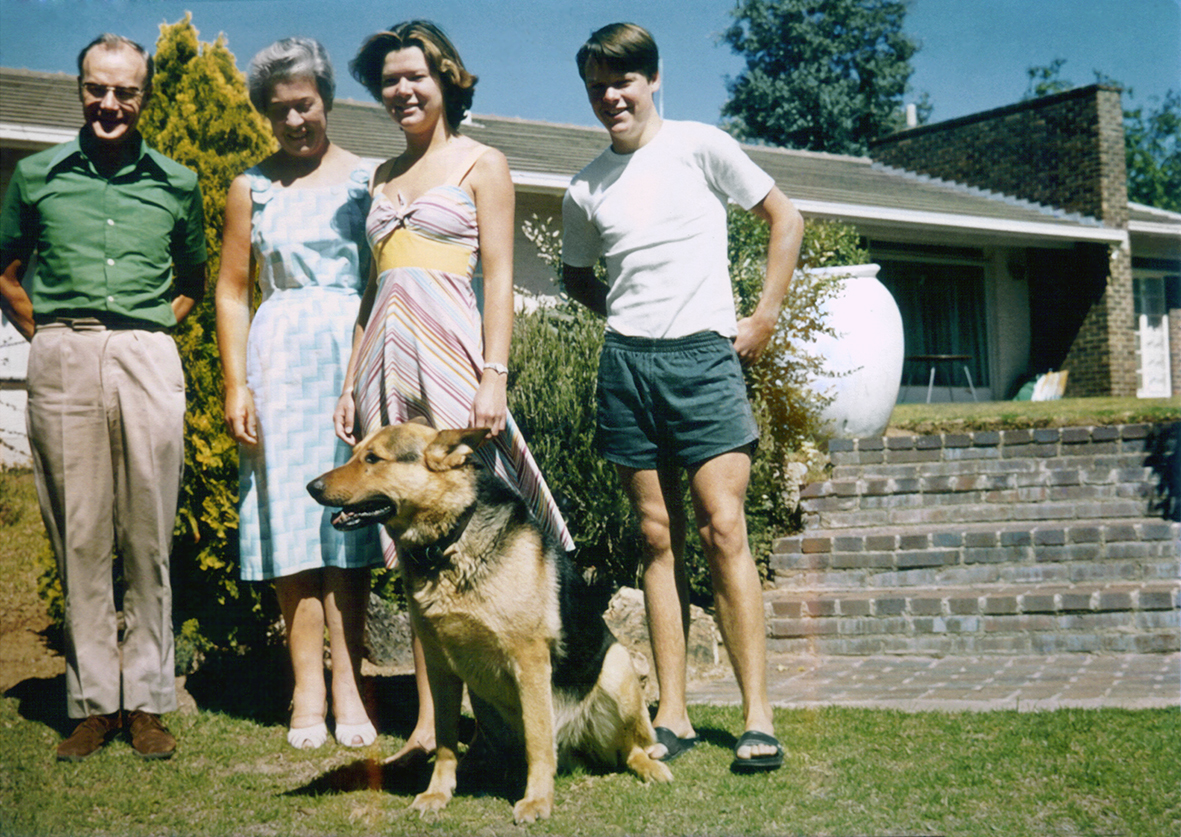
\includegraphics[width=0.8\textwidth]{photos/bray-family.jpg}\label{bray-family}}
    \\
  \end{tabular}
  \caption{Family years.}
  \label{family-years}
\end{figure}

% \begin{figure}
%   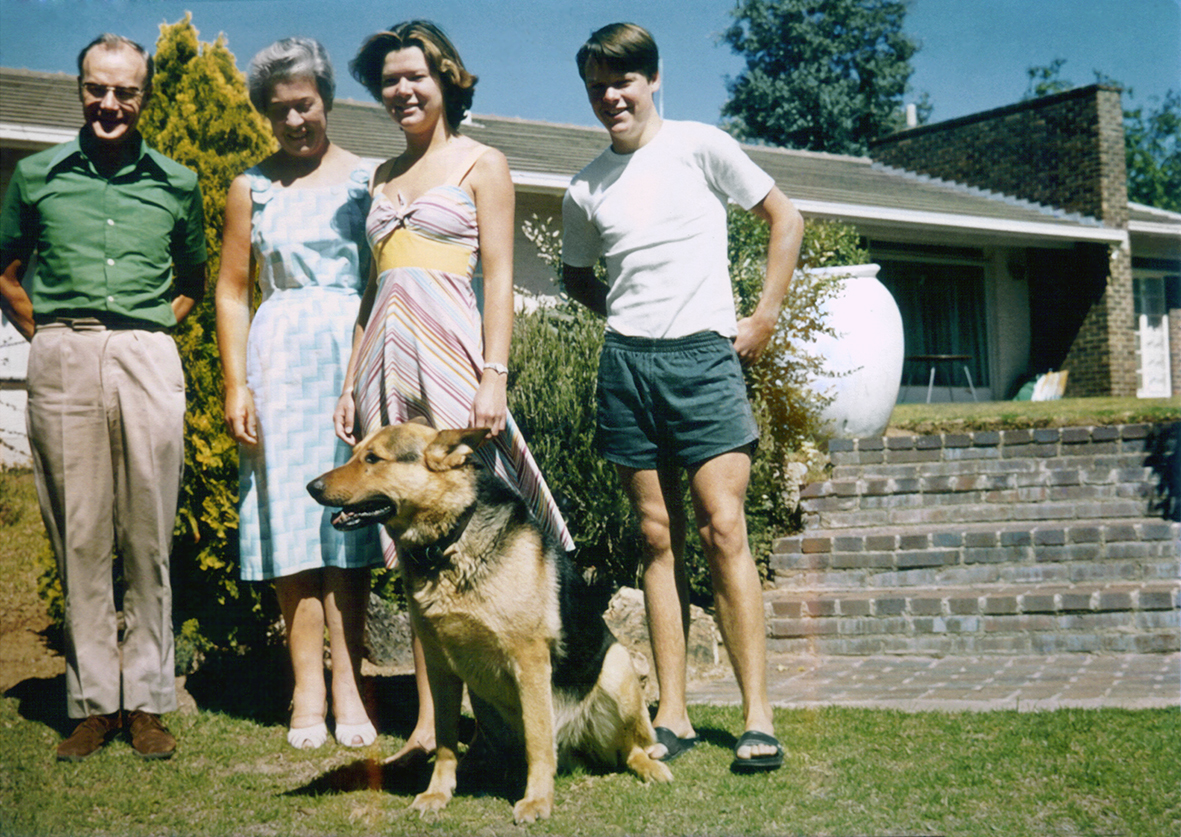
\includegraphics[width=\textwidth]{photos/bray-family}
%   \caption{The Bray family in Johannesburg.}
%   \label{bray-family}
% \end{figure}

Once more we had to look for schools and we chose Roedean\footnote{An
  offshoot of the Brighton school} for Elizabeth and St. John's for
Richard. Elizabeth was a day girl and I drove her to school and back
every day. The only way to apply for Richard to go to St. John's
college was to enroll him as a weekly boarder. He was only 8 (see
Picture~\ref{richard-school}).

% \begin{figure}
%   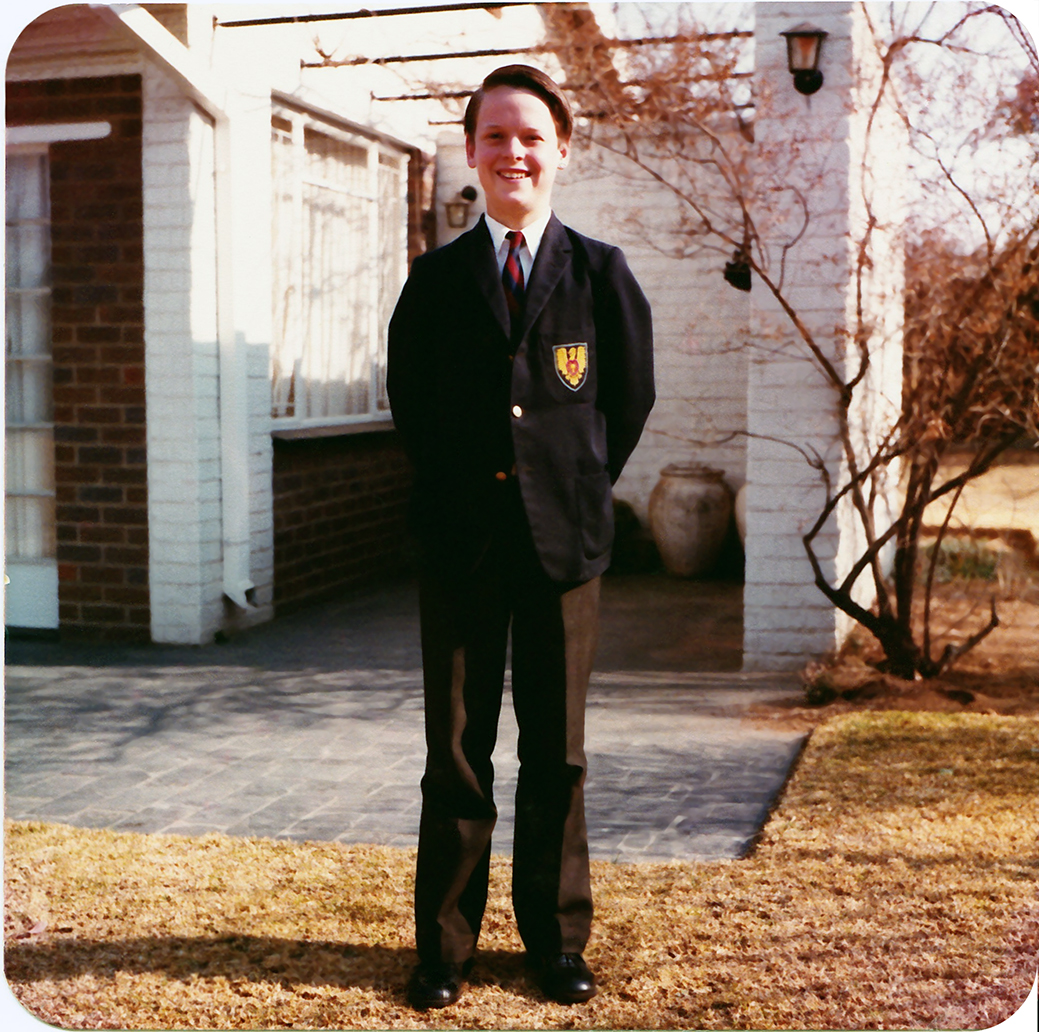
\includegraphics[width=\textwidth]{photos/richard-school}
%   \caption{Richard on his way to schoool.}
%   \label{richard-school}
% \end{figure}

Richard's love of cricket followed him through the school and he was
always chosen for the A-team as he moved up through the age groups. He
was a medium-pace bowler -- and very accurate -- and was awarded 2
hat-tricks during his career. We were very proud when he gained his
cricket colours in 1978.

Richard had decided on a hotel career and having gained his Matric, he
went immediately into hotel training. Starting off with Holiday Inn,
his first place was Secunda where he met his first wife and they were
to have 2 children. Unfortunately the marriage failed; they were both
too young and Richard needed time to develop his career. A junior
trainee is very much looked down upon but he stood his ground and had
gradual promotions to other Holiday Inn hotels, becoming more
confident and assured. Tony and I visited him in every one of the
hotels he worked in and, of course, this allowed us to see many parts
of the country. He progressed to Sun International and The
Sheraton. He met Pat, who was to become his second wife, and they
settled eventually in Cape Town, which is now his headquarters for he
is now operations manager for the Premier Group. Pat already had a
son, Robin, and their son, Bradley, was born in 1997. Giving us 4
grandchildren but more to come!

Elizabeth did well all through Roedean and gained a good
Matric. Immediately she embarked on her nurses training by choosing to
study nursing and complete a BSc. degree -- studying for long hours
and nursing at the Johannesburg hospital. This was a gruelling
4~years (see Picture~\ref{elizabeth-nurse}).

\begin{figure}
  \centering
  \begin{tabular}{cc}
    \subfloat{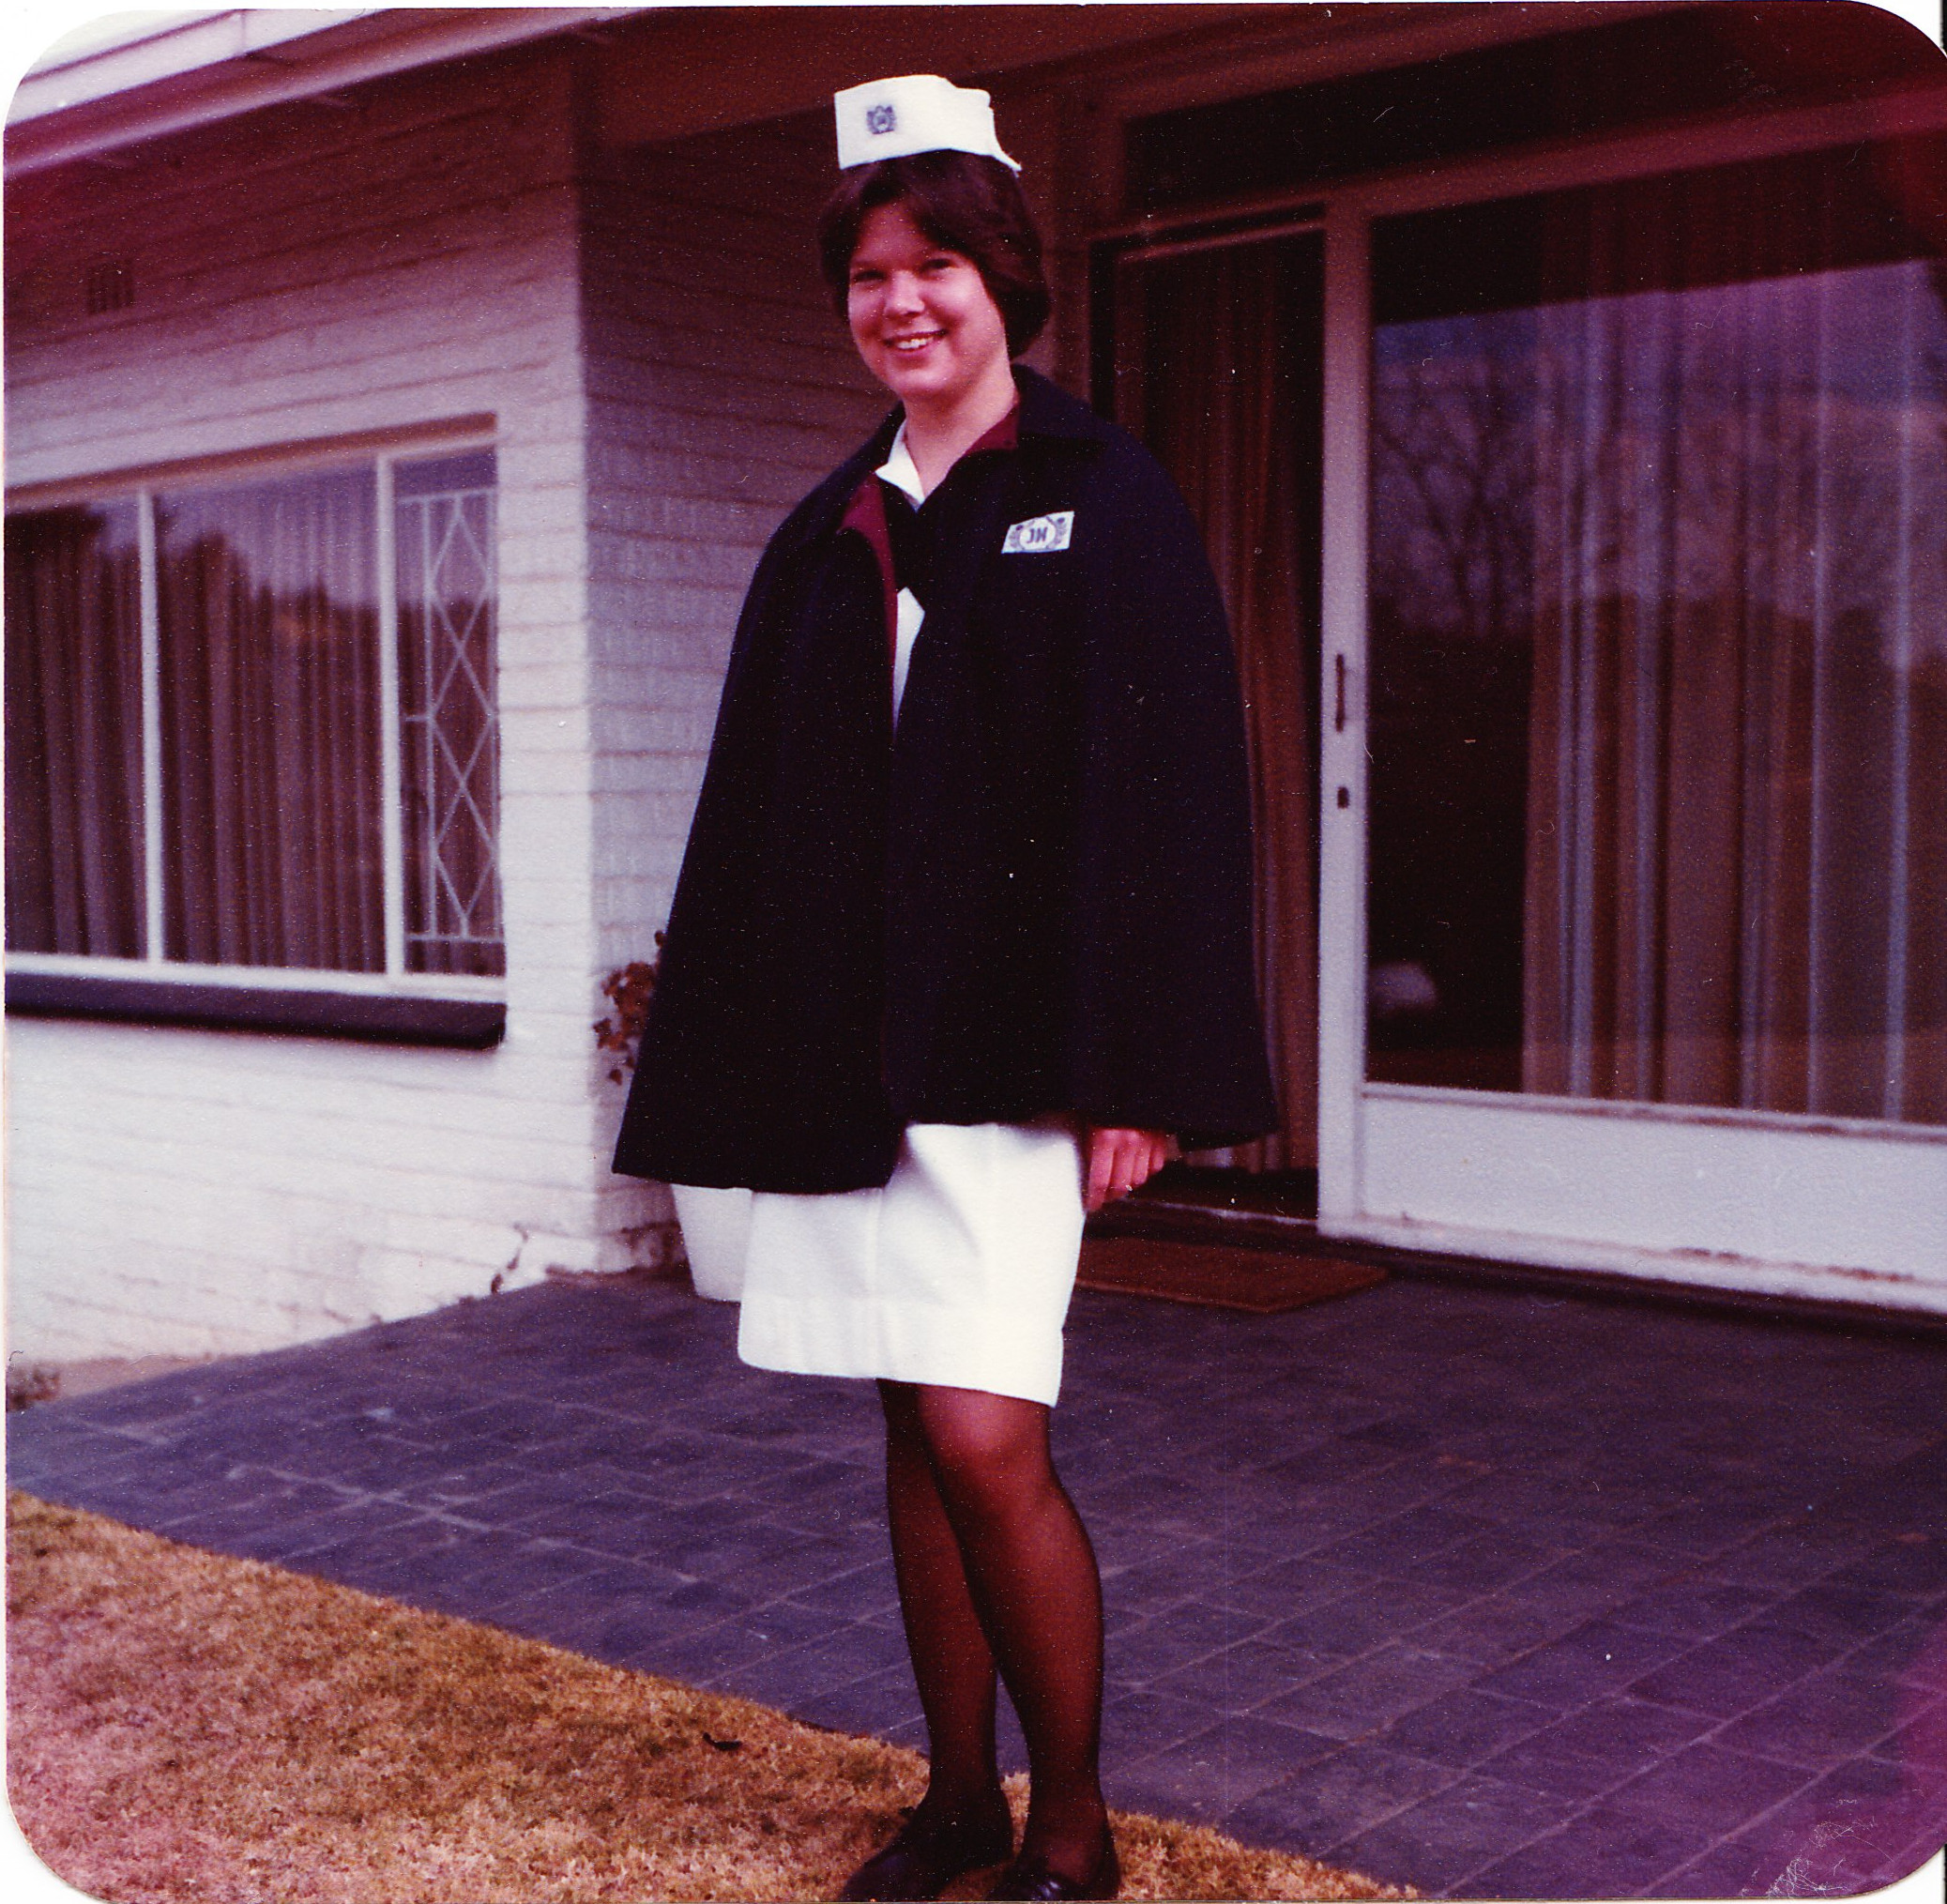
\includegraphics[width=0.45\textwidth]{photos/elizabeth-nurse.jpg}\label{elizabeth-nurse}}
    &
    \subfloat{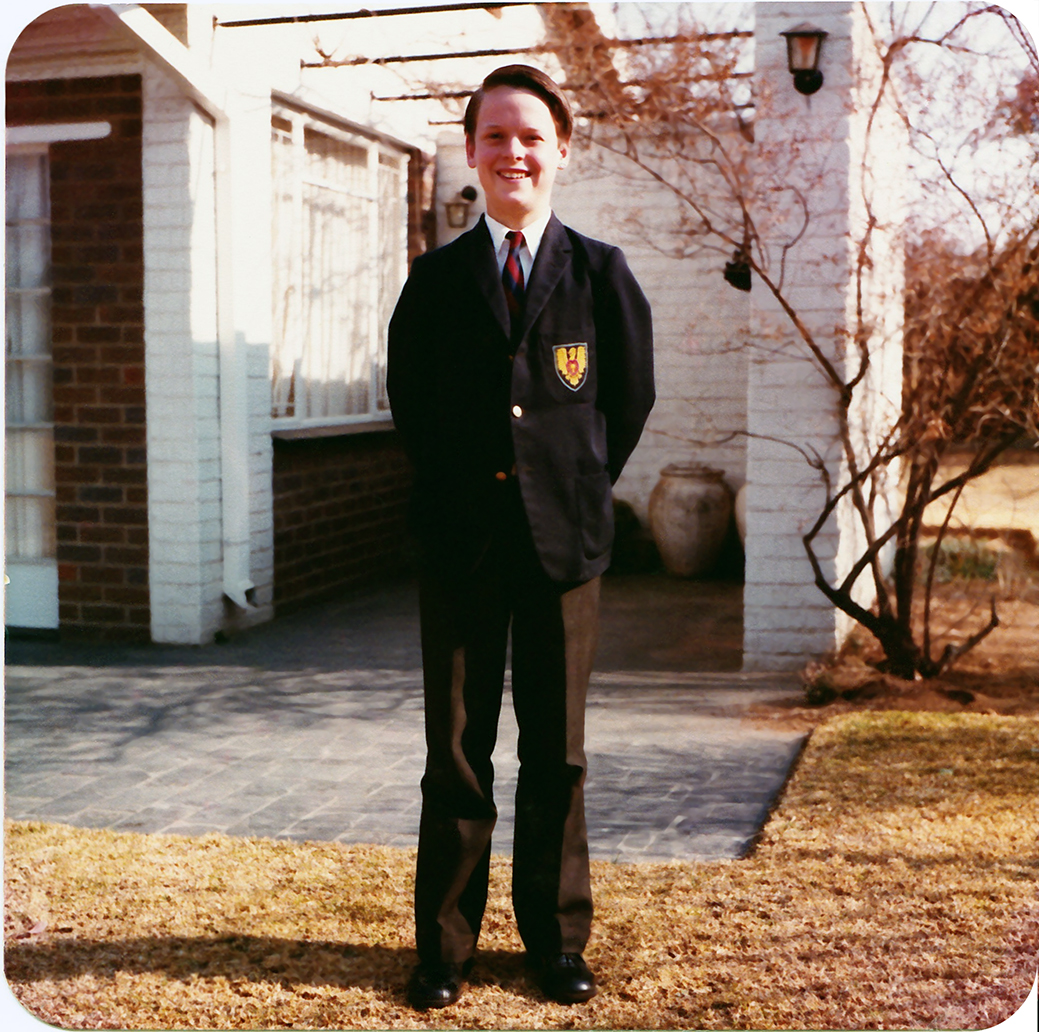
\includegraphics[width=0.45\textwidth]{photos/richard-school.jpg}\label{richard-school}}
    \\
  \end{tabular}
  \caption{Elizabeth (aged 18) \& Richard (aged 16).}
  \label{children}
\end{figure}

% \begin{figure}
%   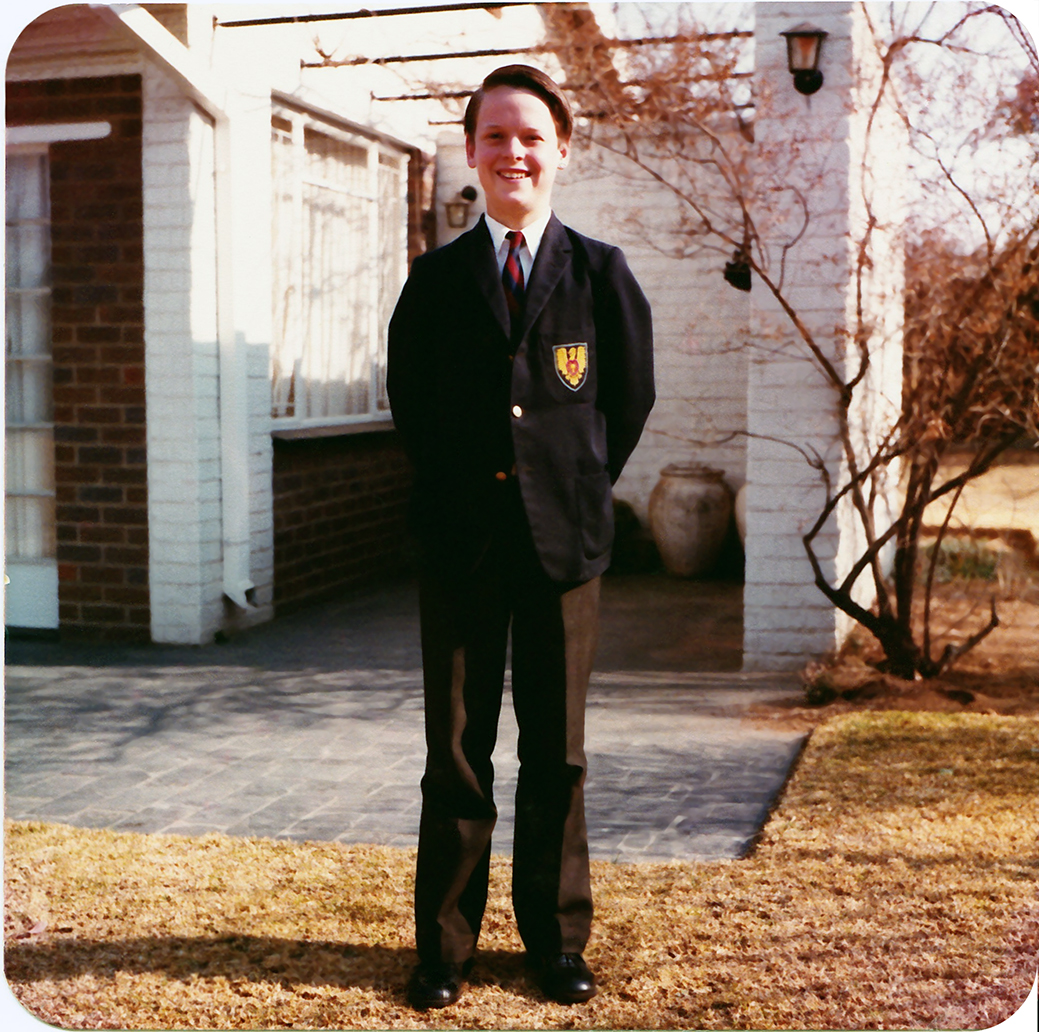
\includegraphics[width=\textwidth]{photos/richard-school}
%   \caption{Richard on his way to schoool.}
%   \label{richard-school}
% \end{figure}

% \begin{figure}
%   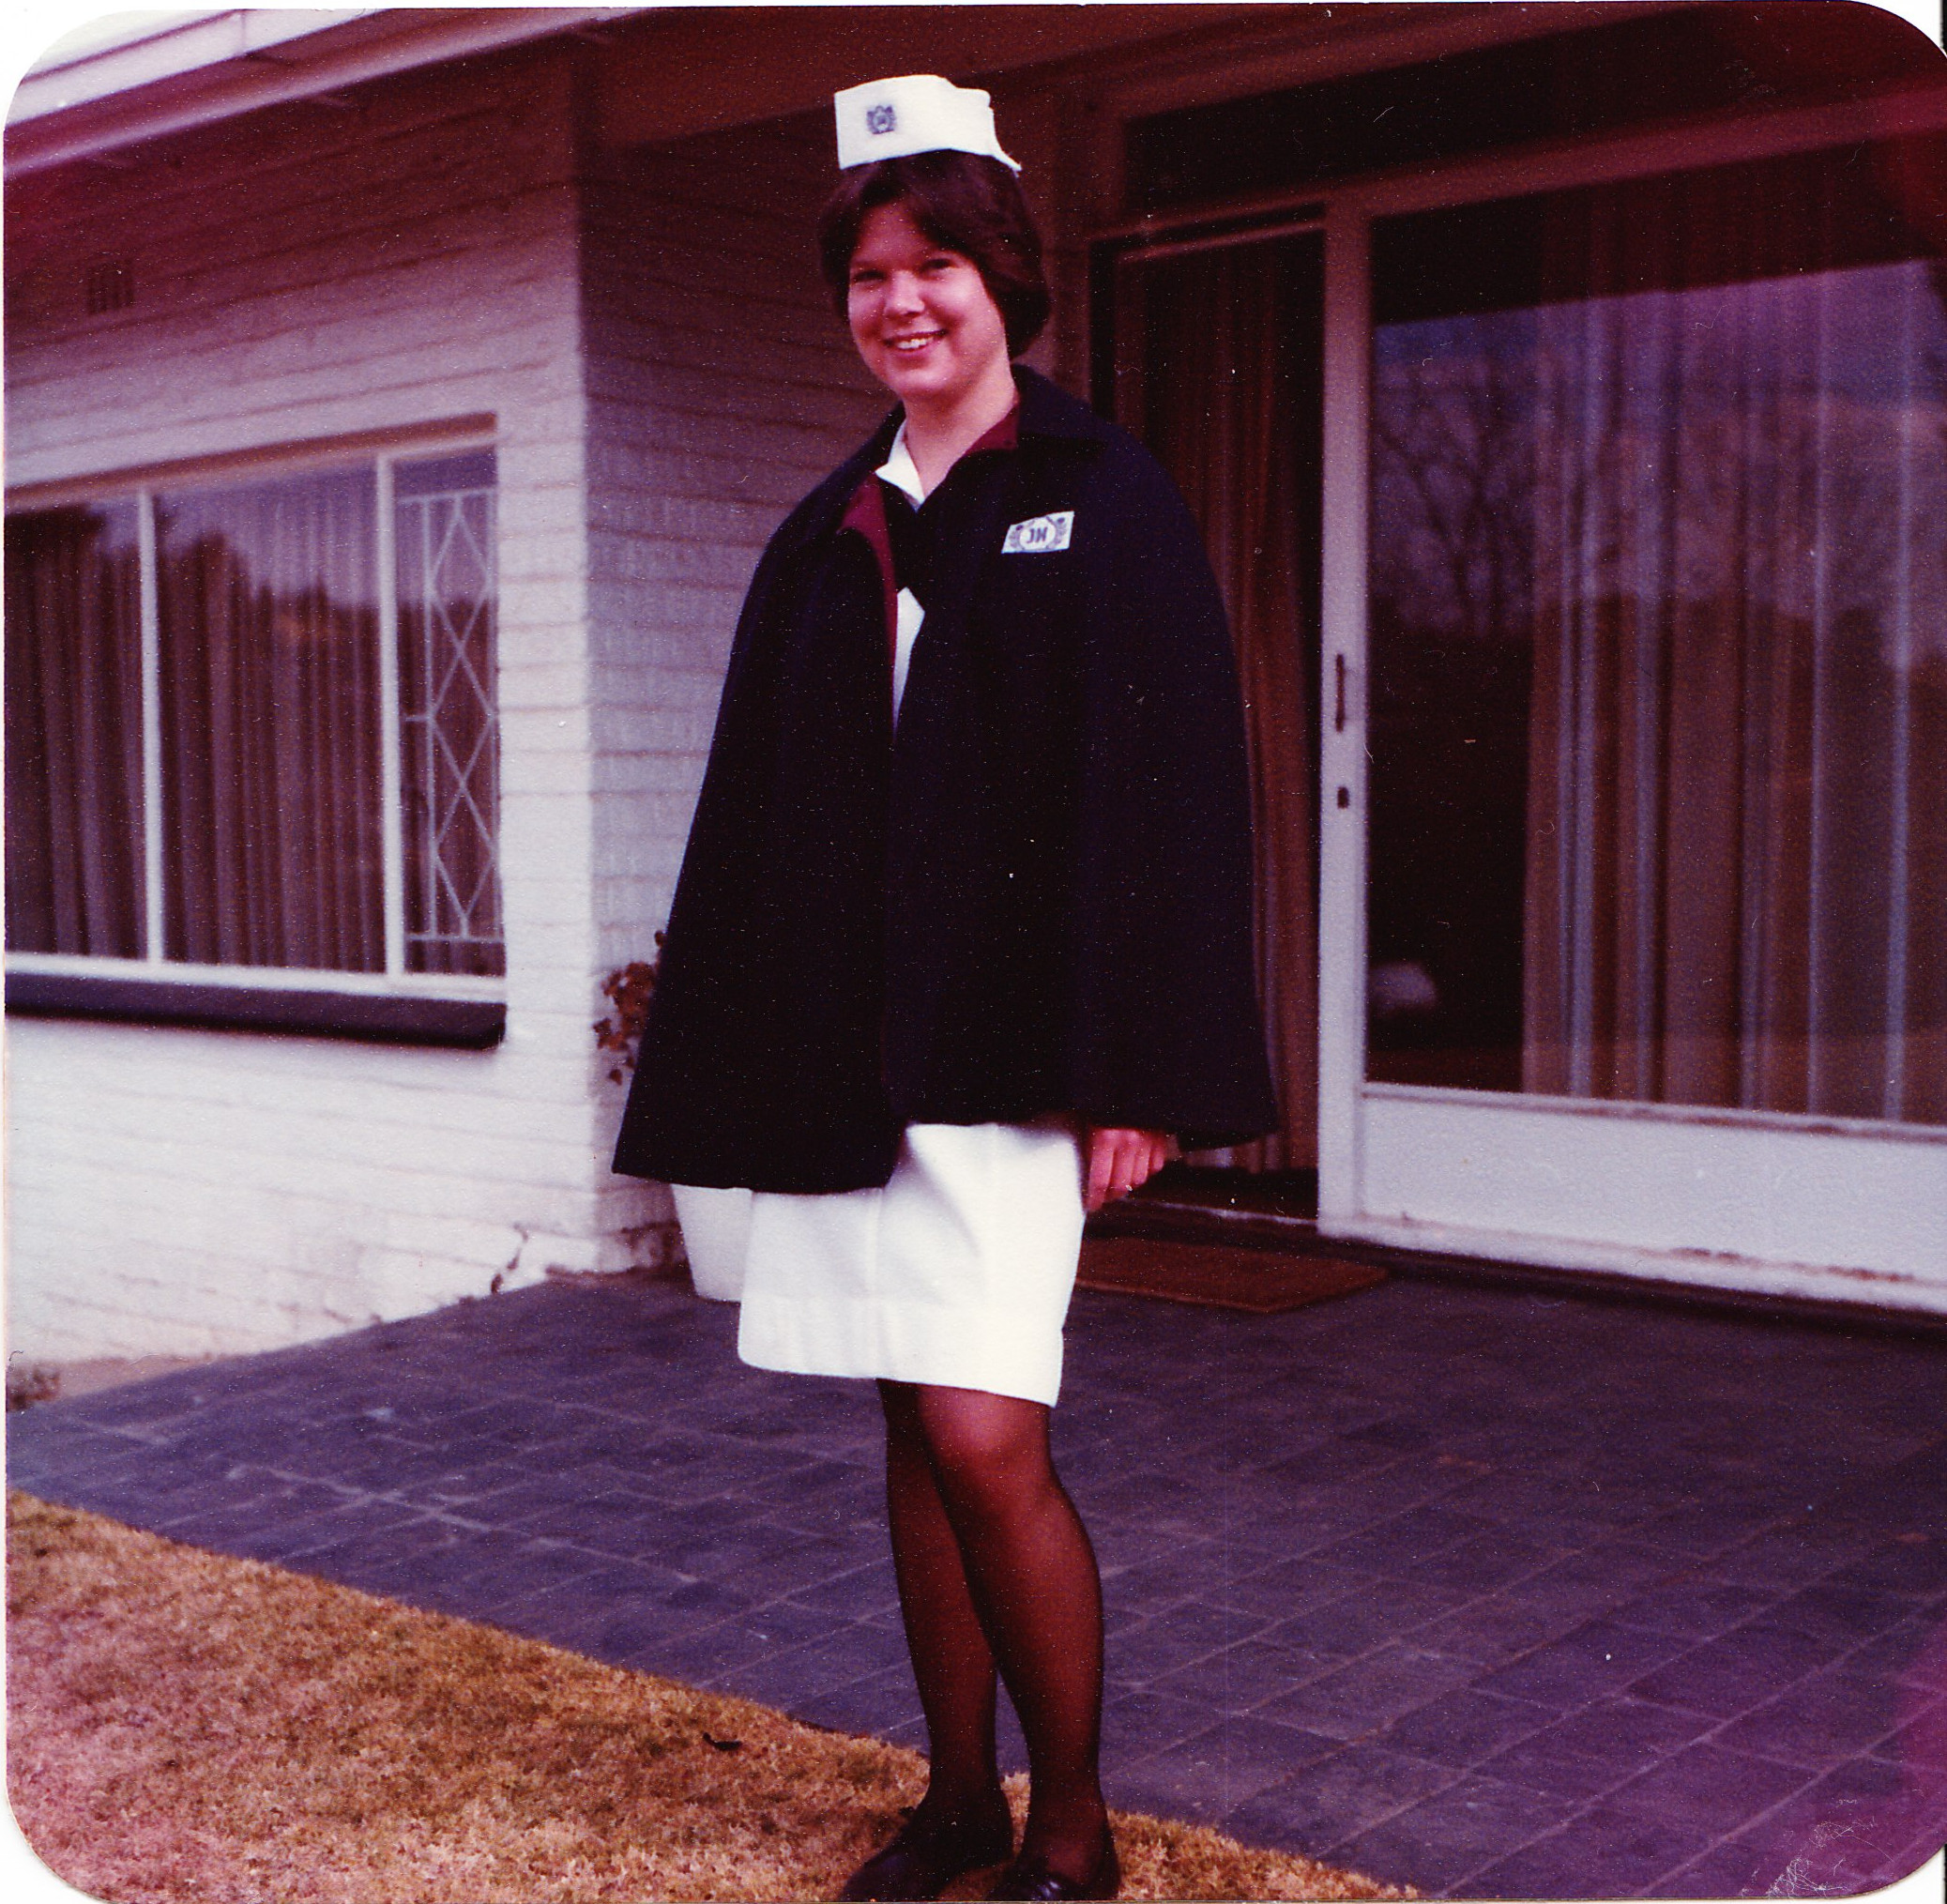
\includegraphics[width=\textwidth]{photos/elizabeth-nurse}
%   \caption{Elizabeth as a nurse.}
%   \label{elizabeth-nurse}
% \end{figure}

While training, she was knocked off a (borrowed) motorbike and had to
be hospitalized with a fractured femur. There she met, and was
attended to, by a young registrar, Matthew Preston, whom she would
eventually marry.

Once she came home from the hospital there was work to be done on the
injured leg. The effort of bending the leg at the knee was terribly
painful and I had to help her with the exercises. I don't know who
suffered the most -- the pain to her was hideous, but she persevered.

Because of her hospitalization, Elizabeth was not able to write her
final exam with the other students. She was permitted to do this later
in a private room.

This was on her 21st birthday and on that very day -- July 21st, 1981
-- Prince Charles and Princess Diana were married. She never did get
to see a video of the wedding! However she succeeded in passing her
final exam. And we were all overjoyed.

Elizabeth and Matthew were married in August 1982 and the wedding took
place in the Roedean chapel; the reception was held at the Wanderers
Club, Johannesburg. It was a very happy occasion but, sadly the
marriage failed after 23~years. During that time 4 wonderful children
were born -- Andrew, Claire, Lisa, and Shaun.

Tony and I suffered a lot of heartache over our childrens' divorces,
but were happy that they have both found happiness. In New Zealand,
Elizabeth was brave enough to resume her studies in nursing and gained
her masters degree in 2012.

It was sad that Tony had to miss this wonderful achievement. He would
have been proud; I found enough pride for both of us. Meanwhile,
Elizabeth continues with her work in ICU.


\chapter{Grandchildren}

Andrew, Claire, Lisa, and Shaun.

Ryan, Kelly-Ann, Robin, and Bradley.

I am of the firm belief that children need their grandparents as much
as the oldies need the younger ones.

I value the friendship and support of my grandchildren very much and I
think mainly because I grew up in the era when the oldies were very
strict (and parents too) and affection did not come very much to the
fore. I love the more free and easy way of living today albeit gone a
little too far regarding discipline etc.

Frankly I dreaded my annual 2~weeks summer holiday with my mother's
mother. She never showed me much affection, dressed always in purple
or black and her hair was scraped into a topknot -- in other words she
was a very severe old lady; she was always old to me.

My other grandmother was vague and disinterested and my grandfather
was always pushing the bible, which did nothing to interest a young
girl.

How much more interest is shown in grandchildren today.

Many mothers go out to work and the oldies have the pleasure and
responsibility of looking after the children and this does form a
remarkable bond.

I have pleasant memories of babysitting with all of Elizabeth's
children.

Once, when Andrew and I were busy with lego, he put into play his
favourite word of the month which was ``obviously''. ``Obviously you
haven't read the instructions properly, Grandma.'' -- he was right --
I seldom read instructions properly (see Picture~\ref{madge-and-andrew}).

\begin{figure}
  \centering
  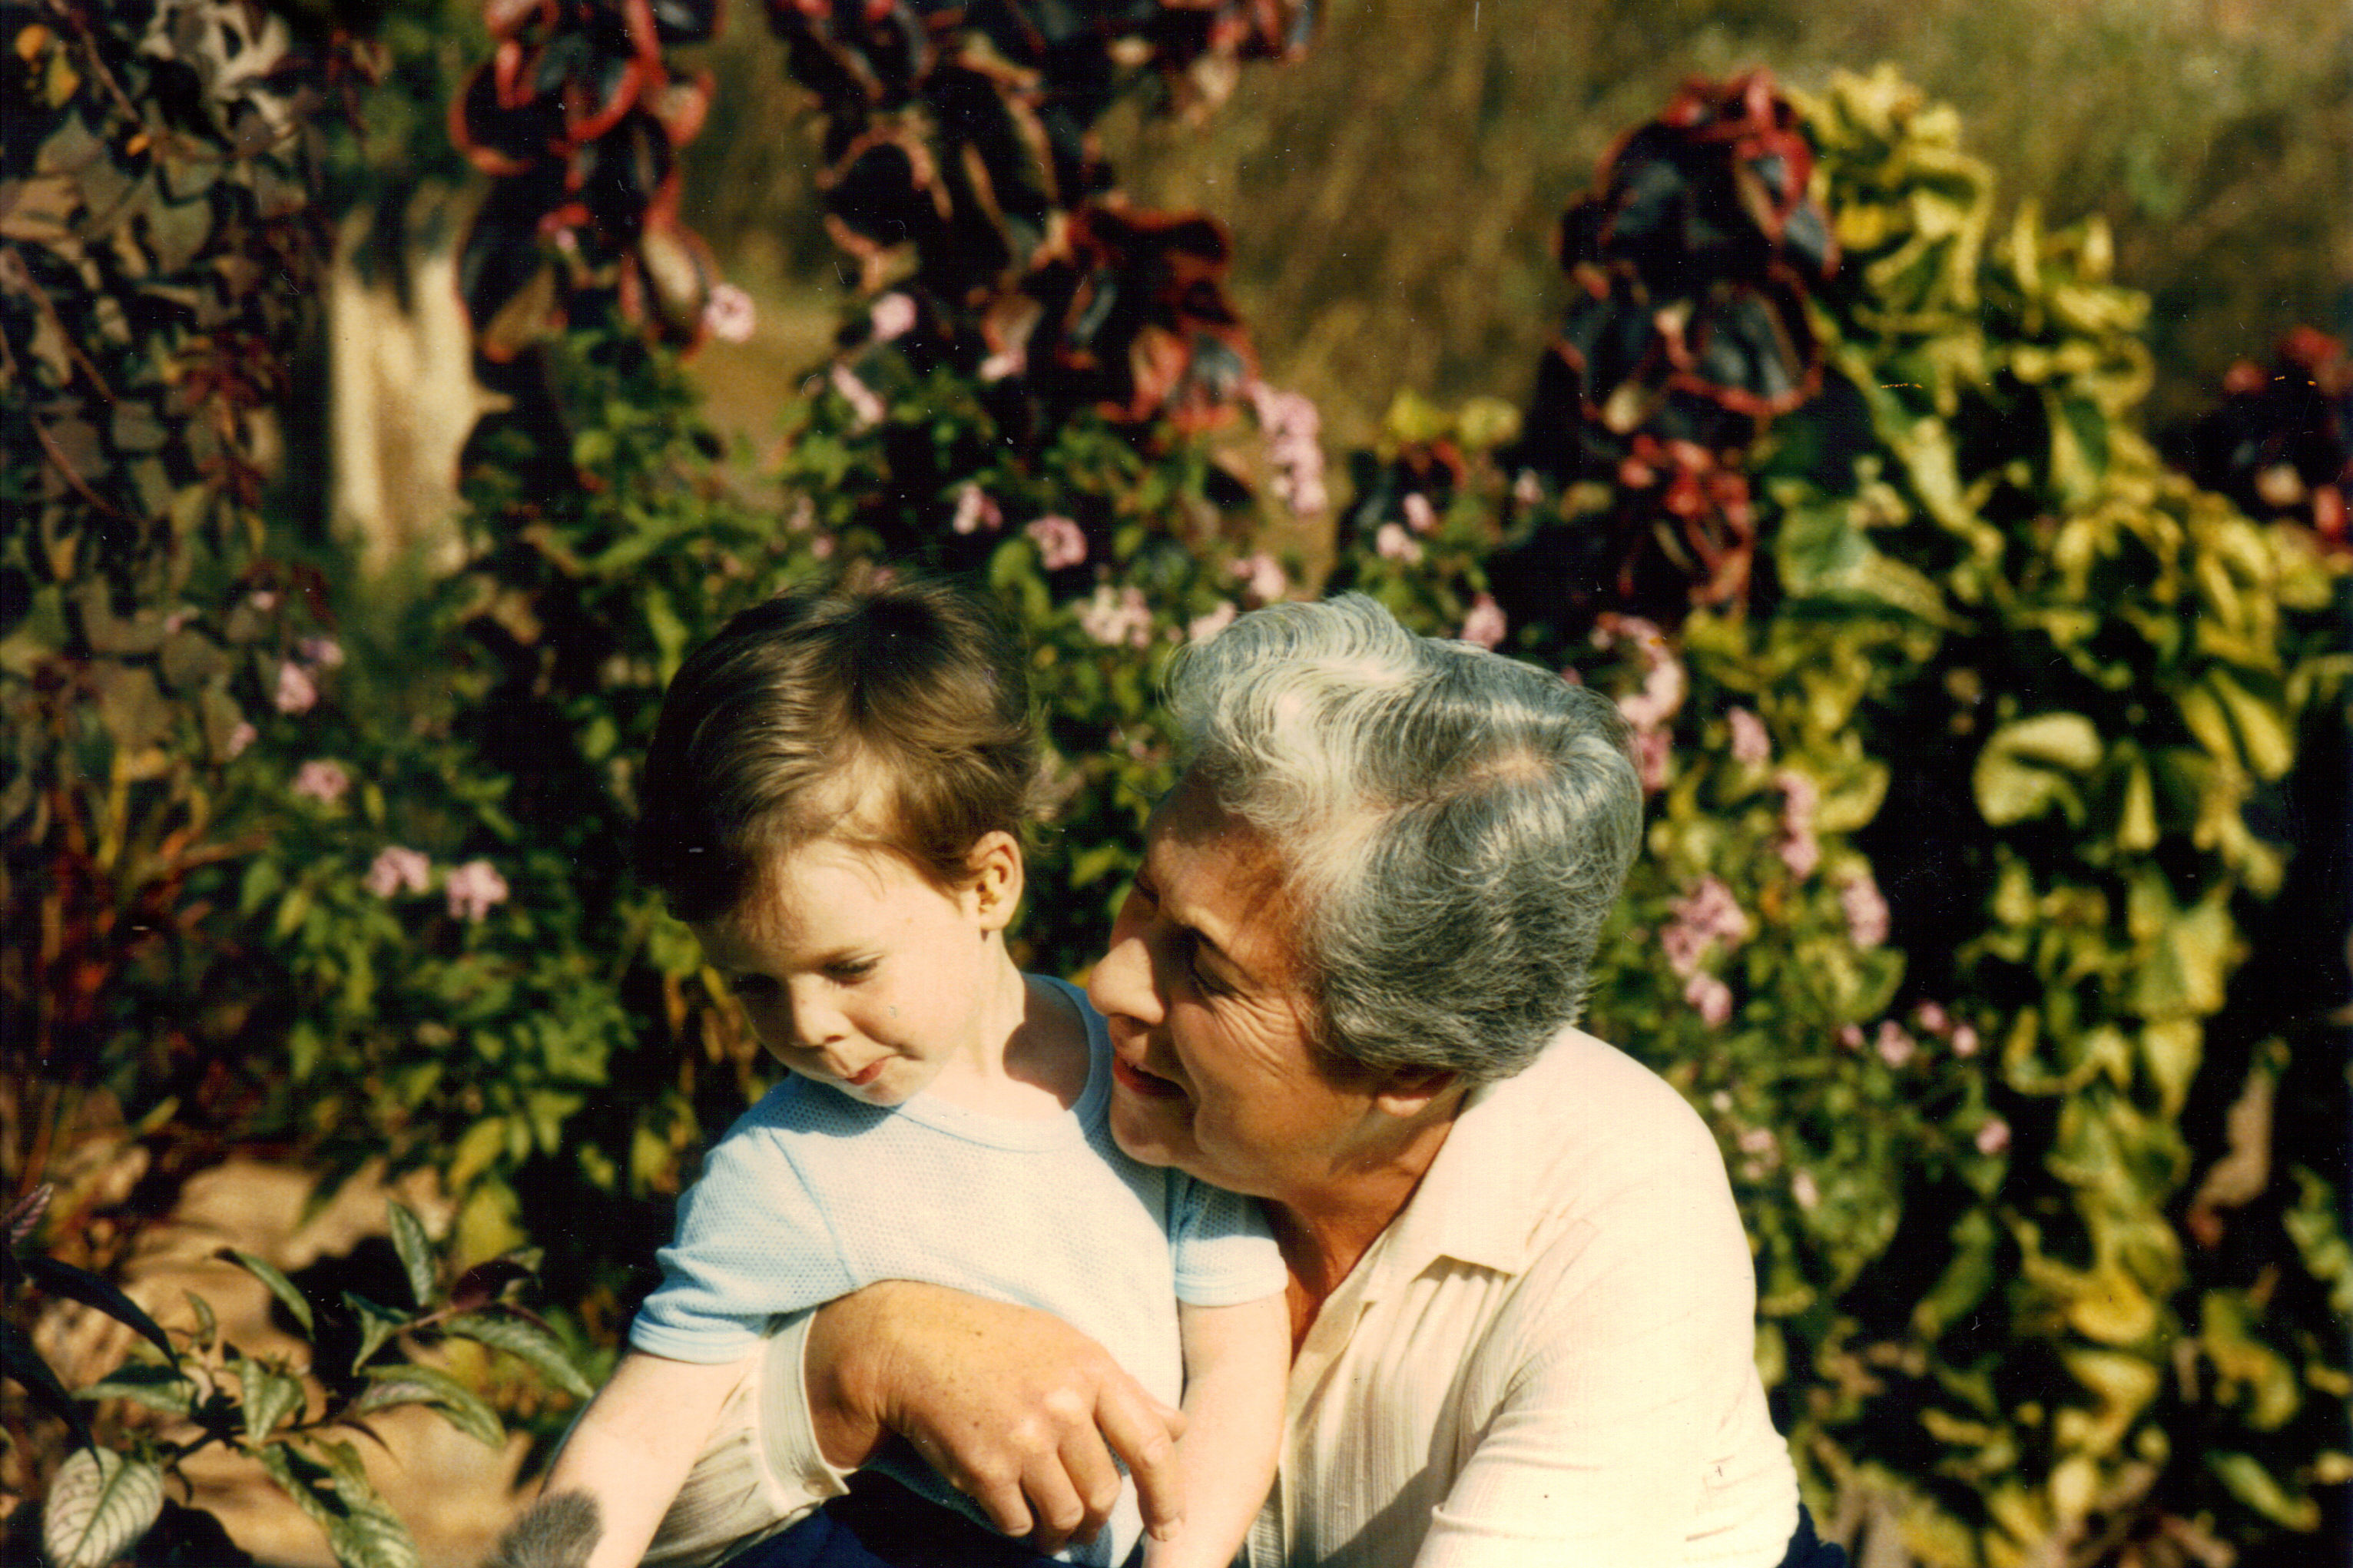
\includegraphics[width=0.9\textwidth]{photos/madge-and-andrew.jpg}
  \caption{Madge holding Andrew.}
  \label{madge-and-andrew}
\end{figure}

This reminds me of another time when I was giving my mother a home
perm. Because I hadn't been concentrating and had omitted one vital
procedure, I had to start all over again. ``Read the instructions
Grandma'' -- Andrew was quite right!

On another occasion I was trying to change the nappy of a very cross
and spirited Claire and I couldn't cope with her screams and kicking
legs. Andrew said ``Move over, Grandma, I can handle this.'' And so he
did with practiced ease.

He must have thought me a real dimwit at times but he never held it
against me. It was interesting for Tony and me to follow his progress
through school and toward adulthood. He achieved his BSc. in 2005 and
then moved on to his PhD without having to write his Masters.

Tony, being of a mathematical mind, was so proud of Andrew and they
had some serious discussions. What a good thing that he took some of
Tony's brains and not mine.

How lucky I am that he and Shaun have got my memoirs into shape to
produce an attractive -- and I hope readable -- book. He is launched
into a successful career but it is beyond me to understand exactly
what he is doing!

Claire is next in line for comment. She was a beautiful girl -- and
still is. We got on very well until things went sadly wrong. The
family had spent the day with us in Winston Park and, for some reason,
Claire chose to spend the night with us and we made up a bed for her
in our bedroom. We were woken up by the sound of a very loud
howl. Claire was sitting up in bed, clearly distressed and not knowing
where she was -- poor little thing. After a drink and some comfort I
took her into bed with me -- I don't know what we did with grandpa --
but the rest of the night was most uncomfortable for she kicked and
fidgeted and I was thoroughly glad to see the morning!

That was the beginning and end of Claire's nocturnal visits but she
remained very precious. Her visit to me in 2012 is so memorable; she
came with Tom (her longtime boyfriend) and, of course, Elizabeth and
we spent some lovely times together, especially during the week we had
in the Drakensberg. We certainly had some wonderful laughs. Claire
schooled me in playing DVDs and CDs but I have never rid myself of
being afraid of doing something wrong with the equipment.

It does not help to realize that I belong to the lost generation of
computer illiterates but we haven't done too badly.

I have found Claire to be a light-hearted, fun-loving, and extremely
practical girl. I am sure she could lift anyone's low spirits and I
hope that sunshine will always be with her; I feel she will never lose
the ability to bring this and happiness into other peoples' lives.

In time Lisa, another beauty, arrived and I enjoyed babysitting with
her. In those early days, we seemed to develop a rapport. Partly, I
think, because of the lullaby I sang to her when she was
unhappy. Always the same tune, ``Wouldn't it be Luverly,'' from My
Fair Lady. She would stop her nonsense and look up at me. She seemed
to recognize the tune and her little eyelids would close. I was very
happy, not only because she had succumbed to sleep, but because the
song had become ours.

Lisa grew and blossomed and, in her teens, went to America on a
student exchange. Back in New Zealand she graduated from a 3 year
course at Victoria University of Wellington and, as I write, is
supremely happy in her first teaching job.

Shaun was 6~months old when the family emigrated to New Zealand so
babysitting with him was mainly watching him sleep; but there were
always his brothers and sisters to be played with or read to.

Tony and I were devastated when the family departed but luckily we
were able to visit them 4 times. But by the time we had re-established
relationships, it would be time for us to leave. We had nice visits
from them when they came for holidays to South Africa and it was good
then to get to know Shaun.

He seemed a very shy boy and I had almost given up hope of
conversations, etc., when, one evening, we were all together playing
some card game and the lights went out. The only thing left for us to
do was to enjoy the candlelight and talk -- and talk Shaun did.  He
was especially interested in talking to Tony and so began a good
rapport. Praise be for electricity failures!

Shaun has not yet decided on a career but he is a good sportsman and
is a fabulous footballer. Who knows? That may even become his career.

\begin{figure}
  \centering
  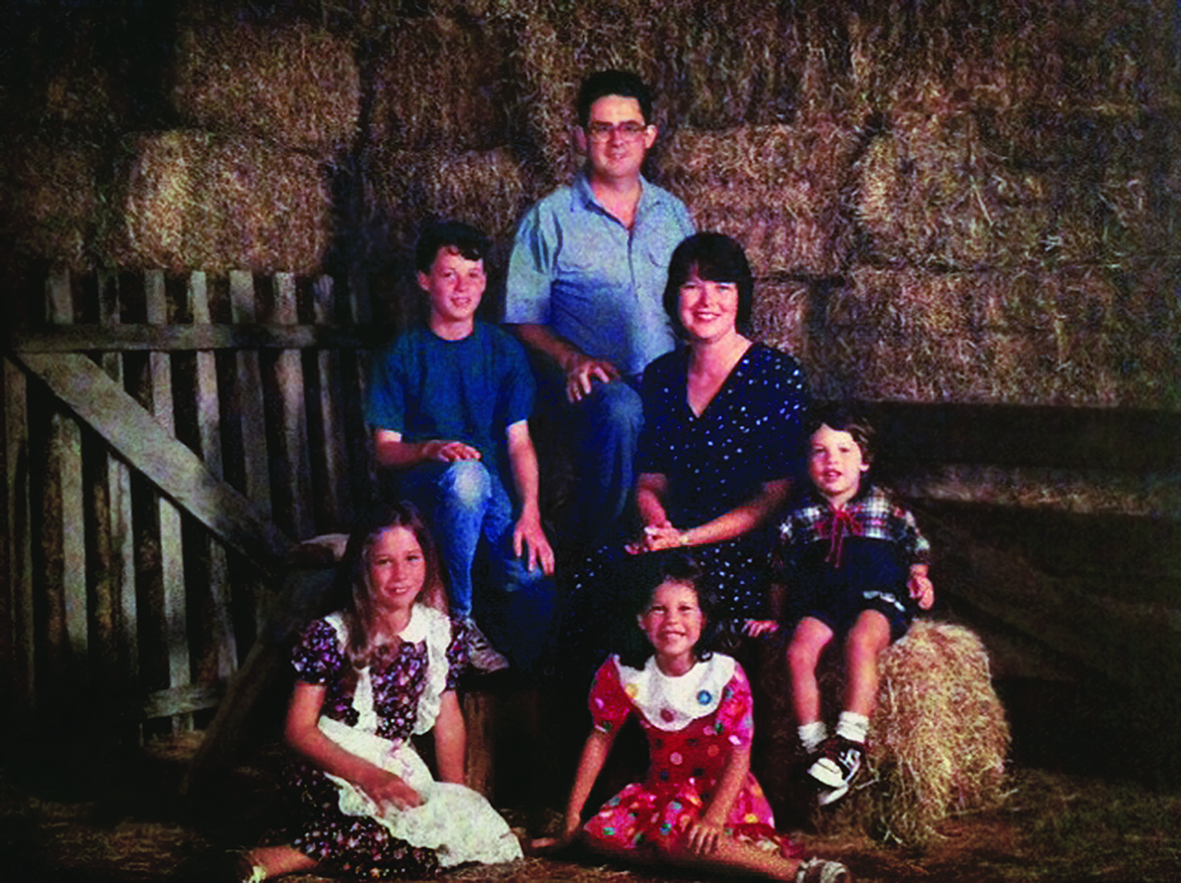
\includegraphics[width=0.9\textwidth]{photos/preston-family.jpg}
  \caption{The Preston family (Rotorua, 1995).}
  \label{preston-family}
\end{figure}

We missed the Preston family terribly when they departed to foreign
shores (see Picture~\ref{preston-family}) but were were not entirely
deprived of grandchildrens' company. We enjoyed the visits of Ryan and
Kelly-Ann (Richard's children) who were living with their mother in
White River. Because of distance we had not seen much of them but we
began to enjoy having them stay during school holidays. It was a long
journey for them to come from White River; having been dropped off in
Johannesburg they then had to face the long bus journey to
Durban. They must have been 10 \& 8 for their first holiday with
us. We were allowed to use a holiday home at Uvongo -- courtesy of
Dave and Muriel Harris -- and we all loved being by the sea for
2~weeks of each holiday (see Picture~\ref{ryan-kelly-ann}).

\begin{figure}
  \centering
  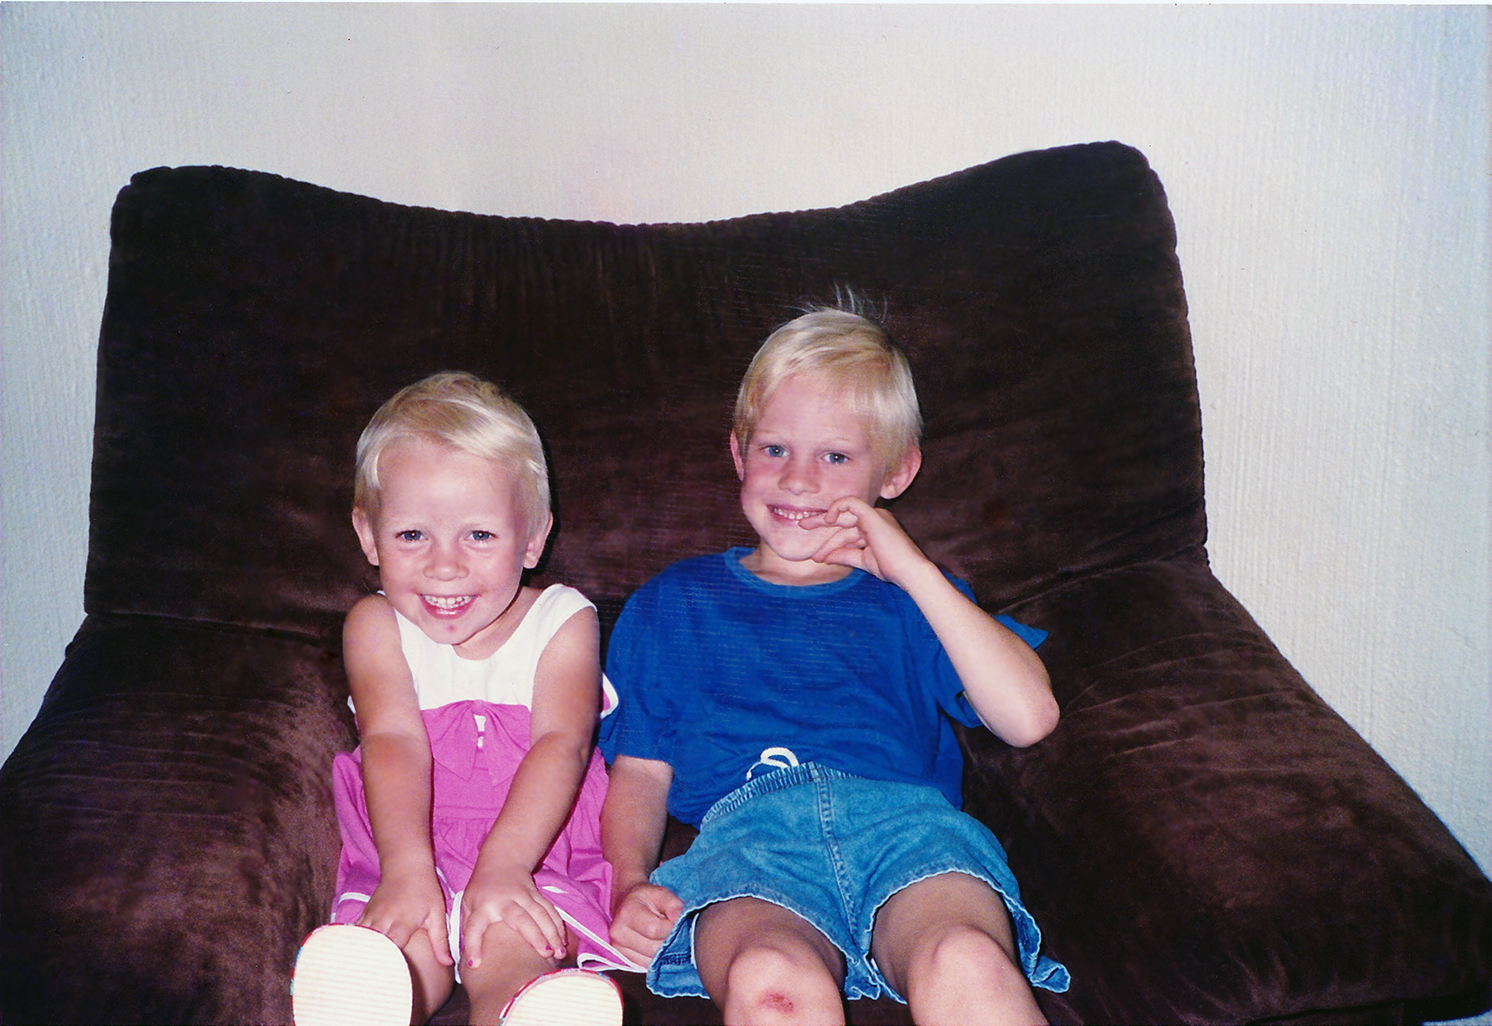
\includegraphics[width=0.9\textwidth]{photos/ryan-and-kelly-ann.jpg}
  \caption{Ryan and Kelly-Ann (1993).}
  \label{ryan-kelly-ann}
\end{figure}

Tony and I would sit and watch them -- rather like Darby and Joan --
when they climbed of rocks catching crabs and loving the sound and
sight of the sea crashing over them (this held quite a bit of
trepidation for me). They were a quarrelsome pair and when we arrived
back home they would fight over who was to have the use of our one and
only electric blanket. Evenings were spent playing Backgammon and they
were very helpful around the house. They had been very well trained by
their mother, Hazel.

We often cooked pancakes establishing a sort of conveyor belt system
with the tossing, adding sugar, and rolling process. It was great fun;
incidentally this cooking fun has also been enjoyed by the Preston
children and, as a matter of fact, by children who wandered into my
kitching in Lagos. There is something about pancakes!

Ryan was boisterous being a boy and we all joined in playing
cricket. He and I played table tennis and I never succeeded in beating
him!

Kelly-Ann was quiet, poised, and capable; I was amazed at her economy
of movement in whatever she was doing.

It was so sad to say goodbye to them and I shall never forget the
tears in their eyes when they pressed their faces to the window of the
departing bus. We have kept in touch as much as possible but phone
calls are not the same as physical contact.

Making good progress through school, Ryan went on to earn a degree in
all aspects of property development at Plymouth University in
England. He took part-time jobs to help with the financial side and
this made me feel very proud.

At university he met Natalie and they graduated together, afterwards
moving to Dubai where they both found good jobs. They are to be
married in Cape Town in March 2014 and I hope to be able to go to the
wedding and to watch the beginning of the greatest adventure of all
time.

Kelly-Ann stays in White River and is working as a swimming
instructor. She has produced a baby girl -- Anne -- my first great
grandchild whom I hope to meet at the wedding.

And so to the children of Richard's second marriage -- Robin (Pat's
son) and Bradley (see Picture~\ref{richard-family}). Robin is making
fantastic progress in the hotel industry; having trained at the Mount
Nelson Hotel in Cape Town, he is now a member of the staff. He is a
real ``peoples person'' with his charm and personality and Tony and I
grew fond of him albeit that we have not had the necessary personal
contact. I am sure he has a great future.

\begin{figure}
  \centering
  \includegraphics[width=0.9\textwidth]{photos/richard-family.jpg}
  \caption{Richard, Pat, Robin, and Bradley (Cape Town, 2013).}
  \label{richard-family}
\end{figure}

Bradley is making good progress through school. Once more there has
been little personal contact but we have had wonderful chats over the
phone. He has a lively and charming personality. It seems highly
possible that he will enter the hotel industry and I wish him luck.
He has an amazing ability to absorb information and to impart it and I
am sure he will become an excellent hotelier.  Good luck, Bradley.


\chapter{Nigeria}

Nigeria lies 6 degrees north of the equator.

It took a while to get used to the unpleasant conditions. The
temperature being around 30 degrees celsius for almost the entire year
and the humidity 80~--~90\%; there was little relief during the night
time but we were fortunate enough to have air-conditioning in the
bedrooms of the lovely house we occupied during our 11 years there
(see Picture~\ref{family-nigeria}).

\begin{figure}
  \centering
  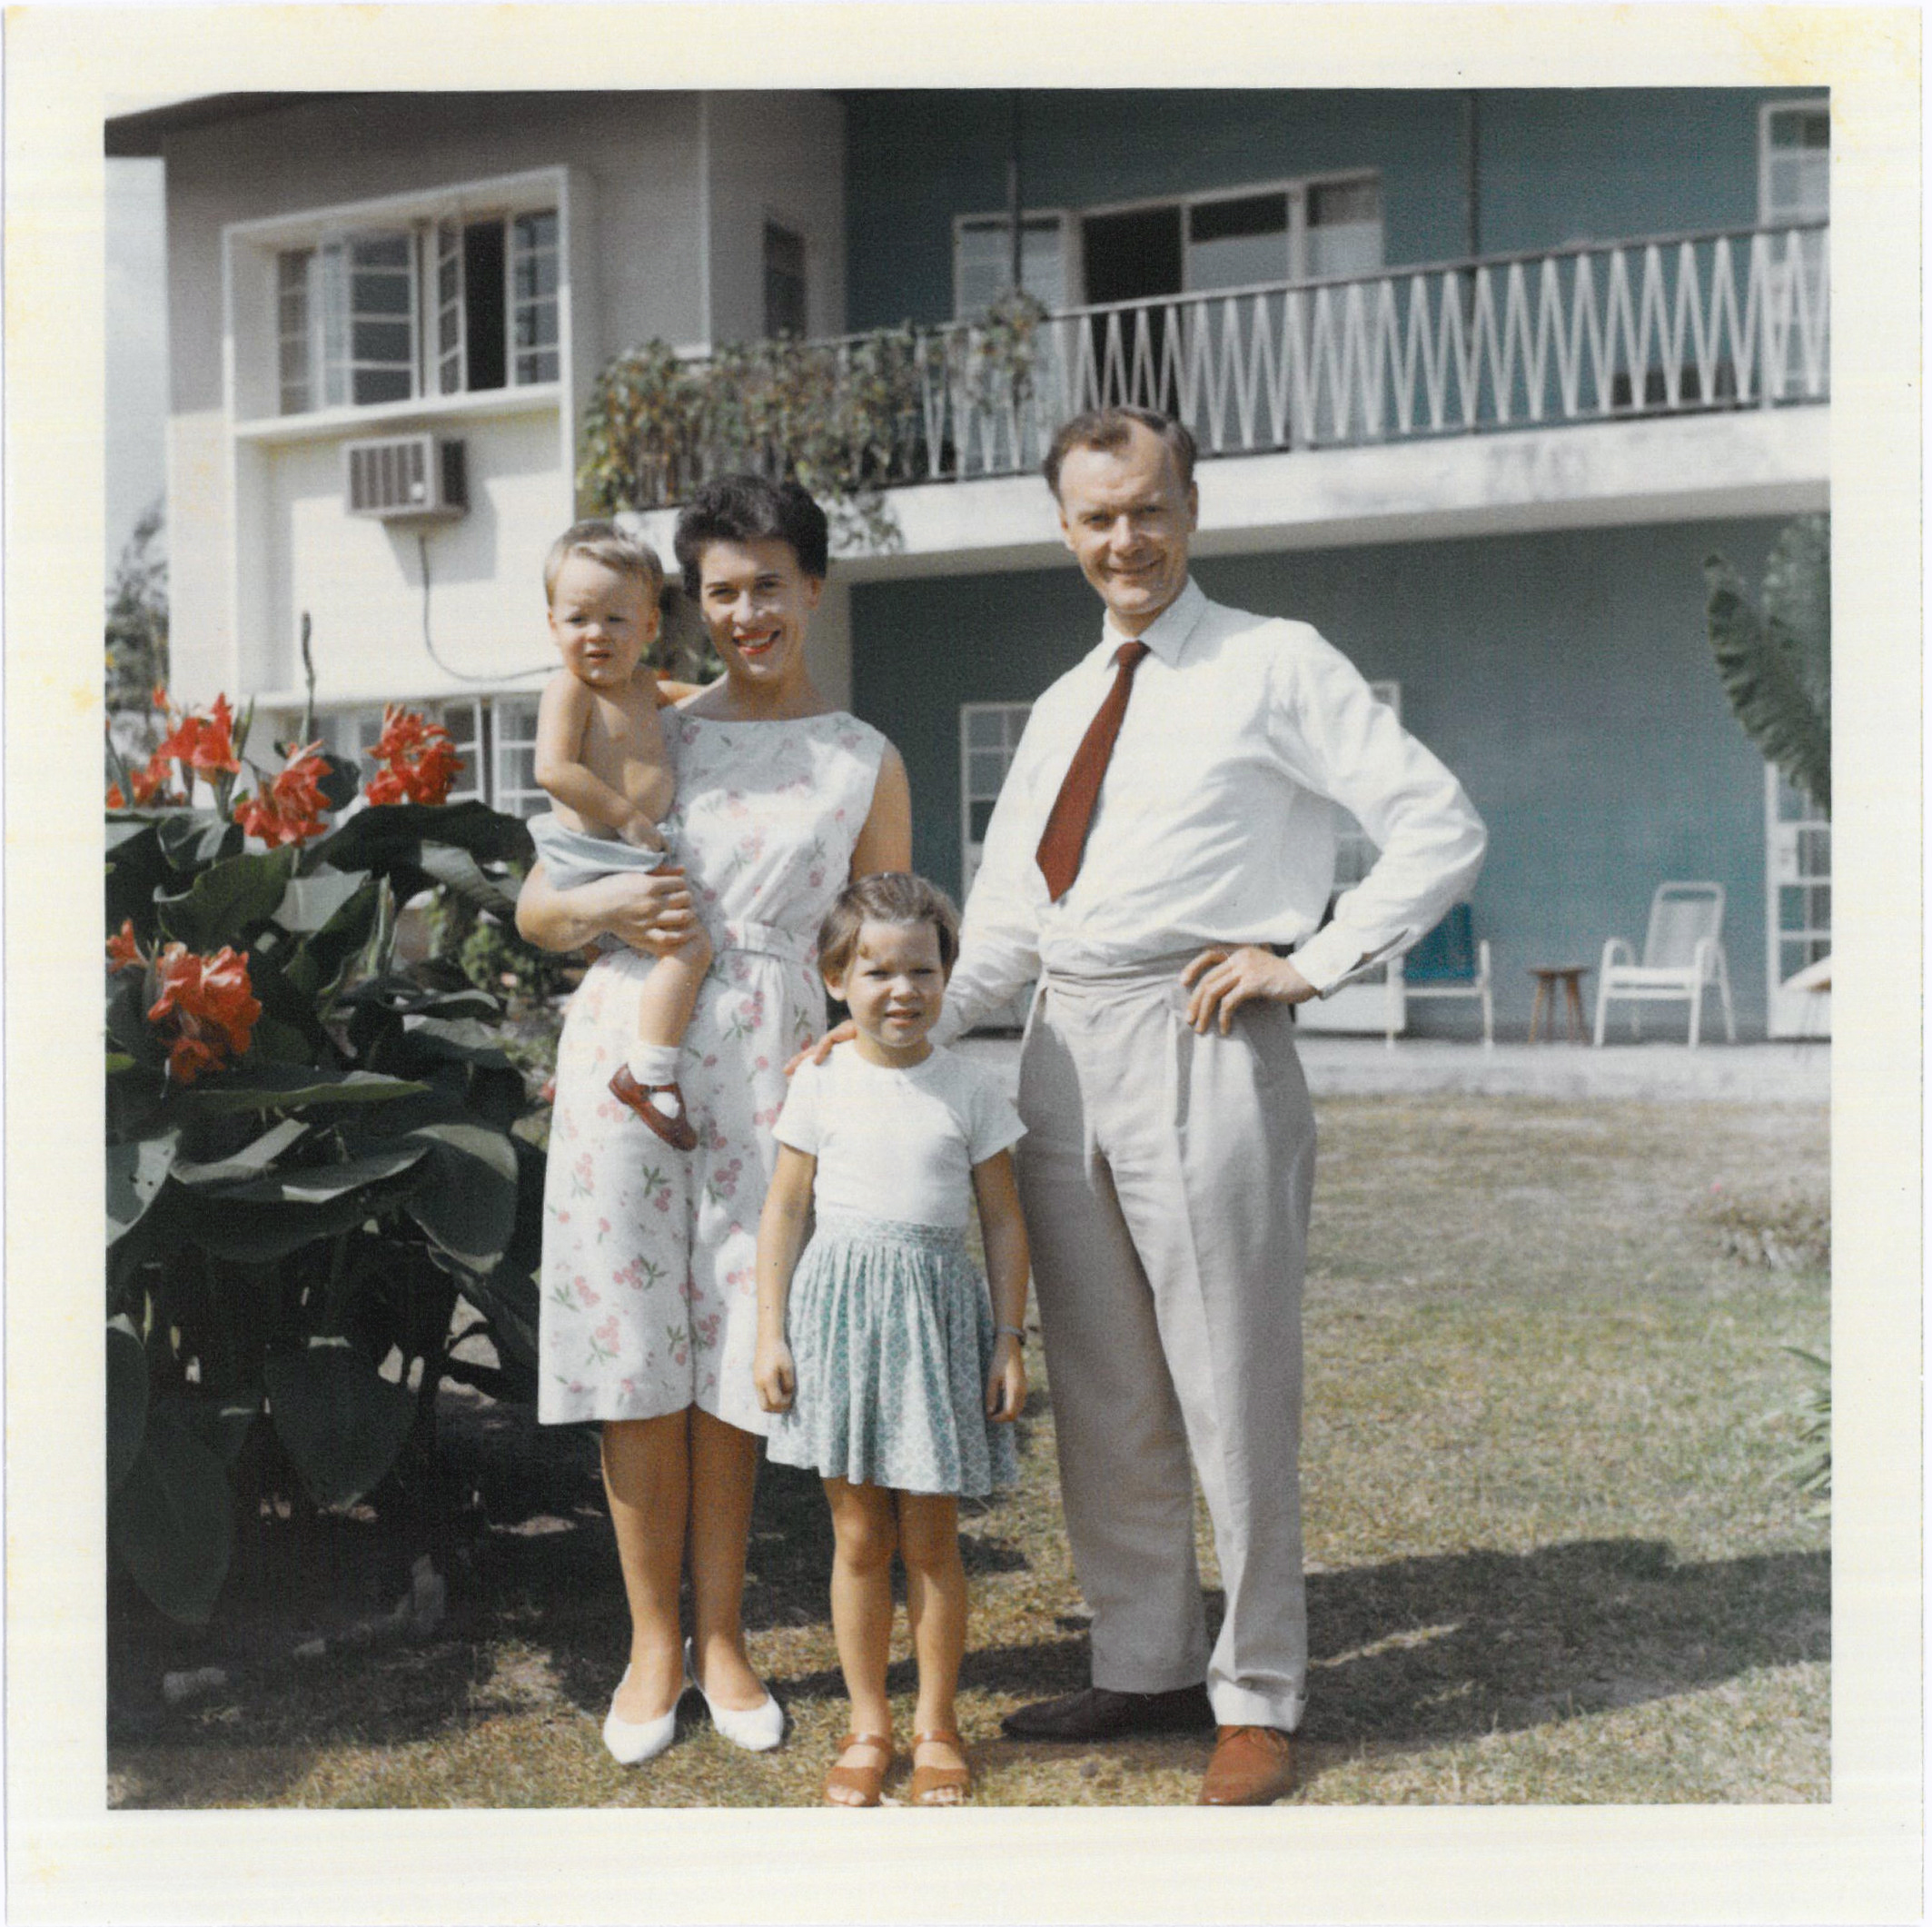
\includegraphics[width=\textwidth]{photos/family-nigeria.jpg}
  \caption{Tony, Madge, Elizabeth, and Richard in front of their house
  in Lagos (1965).}
  \label{family-nigeria}
\end{figure}

With Nigerianisation maintenance of basic services like electricity,
water, etc. fell away and sometimes we would experience cuts of 72
hours. I am pleased to say that, in spite of the lengthy electricity
cuts we only ever lost six ice lollies! And in spite of Audu (our
faithful Muslim cook/steward) opening the fridge door to discuss lunch
not realizing that one gust of that hot humid air would spoil the
contents or cause defrosting.

Audu and I became great friends and would often have discussions about
things in general. He was a good ``all rounder'', even taking an
interest in the garden. He was tall and of good bearing and came from
the north. He belonged to the Hausa Tribe.

He was mystified about the immaculate conception -- ``You know how you
borned Elizabeth. Ma'am.''

I did find things difficult to explain sometimes.

Audu was a good cook and laundry boy.

We would discuss the menu for a dinner party, in spite of his
intelligence, if I forgot to mention some condiment, he would not
include it -- e.g. If I did not mention roast potatoes, they would be
excluded from the roast lamb dinner!

I remember that there was a succession of ``small'' boys (A small boy
would do the cleaning etc: one boy who suffered with B.O. and this was
so overpowering at times that he had to be told to shower and change
his clothes, he would come back smelling of roses but not for long!)

Around December time a wind -- the Harmattan -- would blow off the
Sahara and deposit sand on floors and furniture etc: furniture had to
be dusted several times a day but this was pointless. It was almost a
relief to escape this dry air and get back to the heat and
humidity. The dryness would bring sinus, cough and chest problems. And
I had a problem which was not helped by my pregnancy as I was now
expecting Richard and the early part of 1964 was not pleasing for me.

I did not want to be in the air conditioning during the day times and
I enjoyed sitting in the garden. We overlooked a creek (were we up the
creek without a paddle?!) and then over an island was the Atlantic. We
had the illusion of cool breezes coming off the ocean. It is known as
``the breeze factor'' and it was very comforting.

\begin{figure}
  \centering
  \subfloat{
    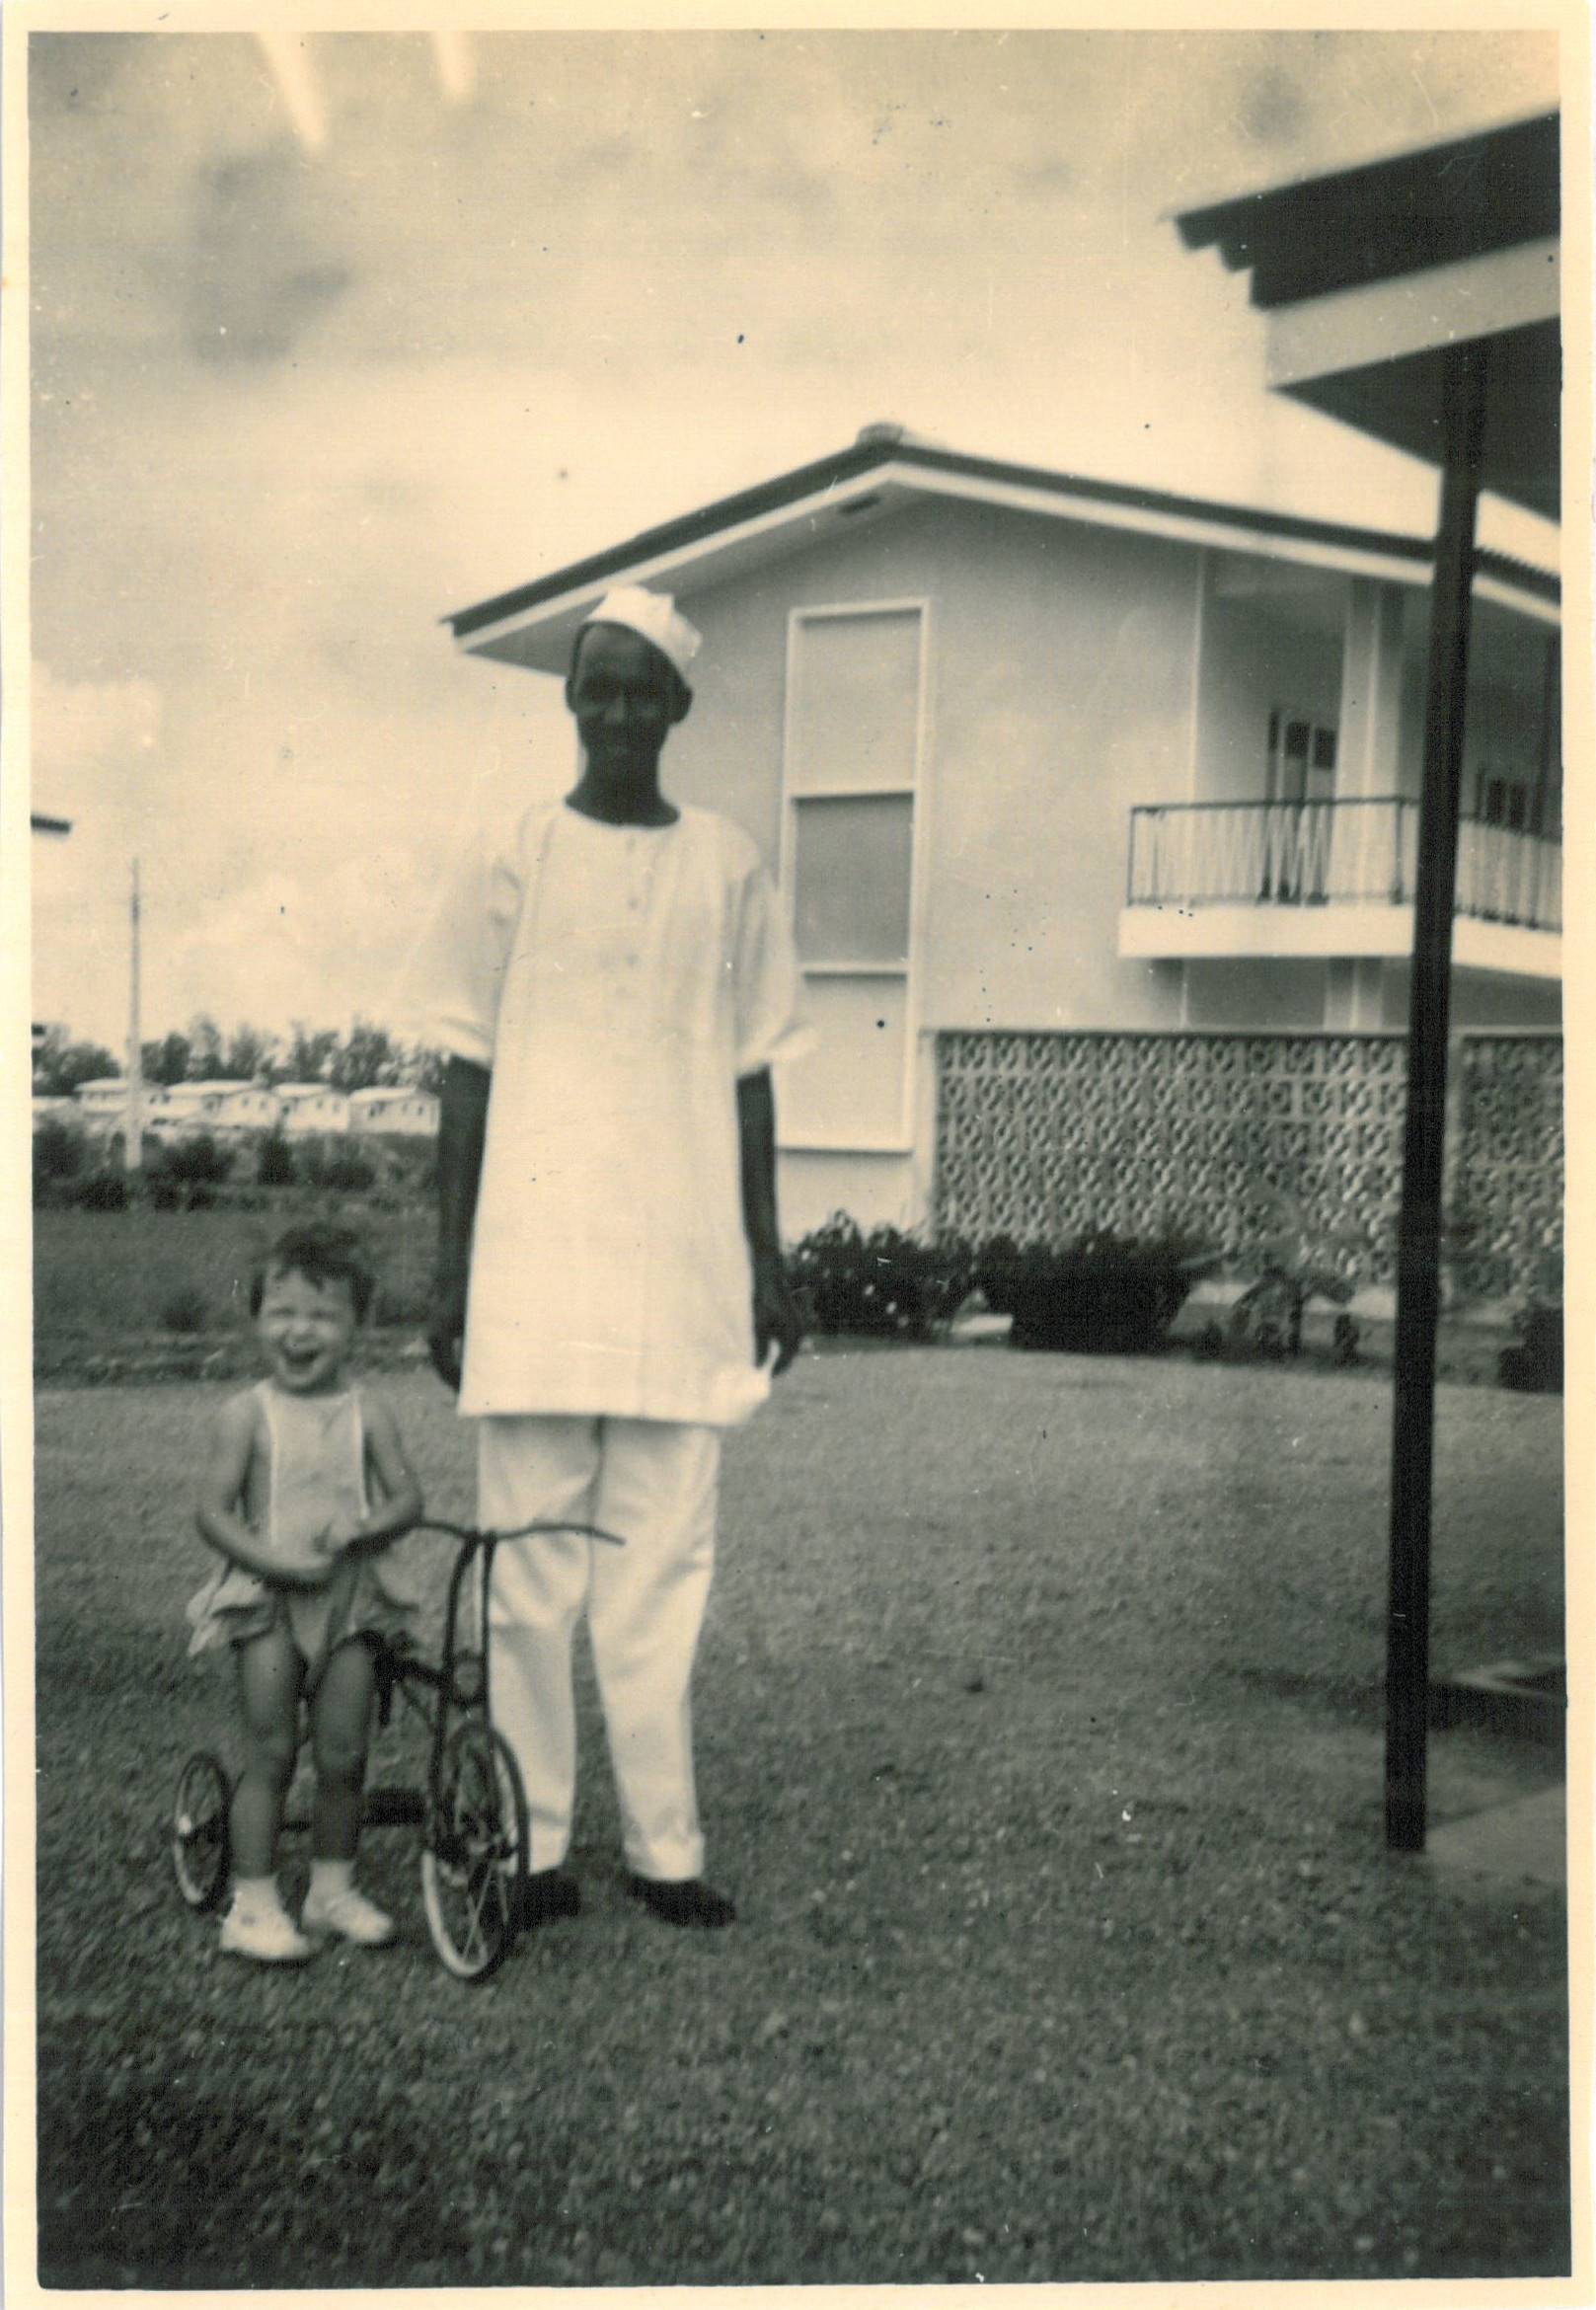
\includegraphics[width=0.45\textwidth]{photos/elizabeth-with-audu.jpg}
    \label{elizabeth-with-audu}
  }
  \subfloat{
    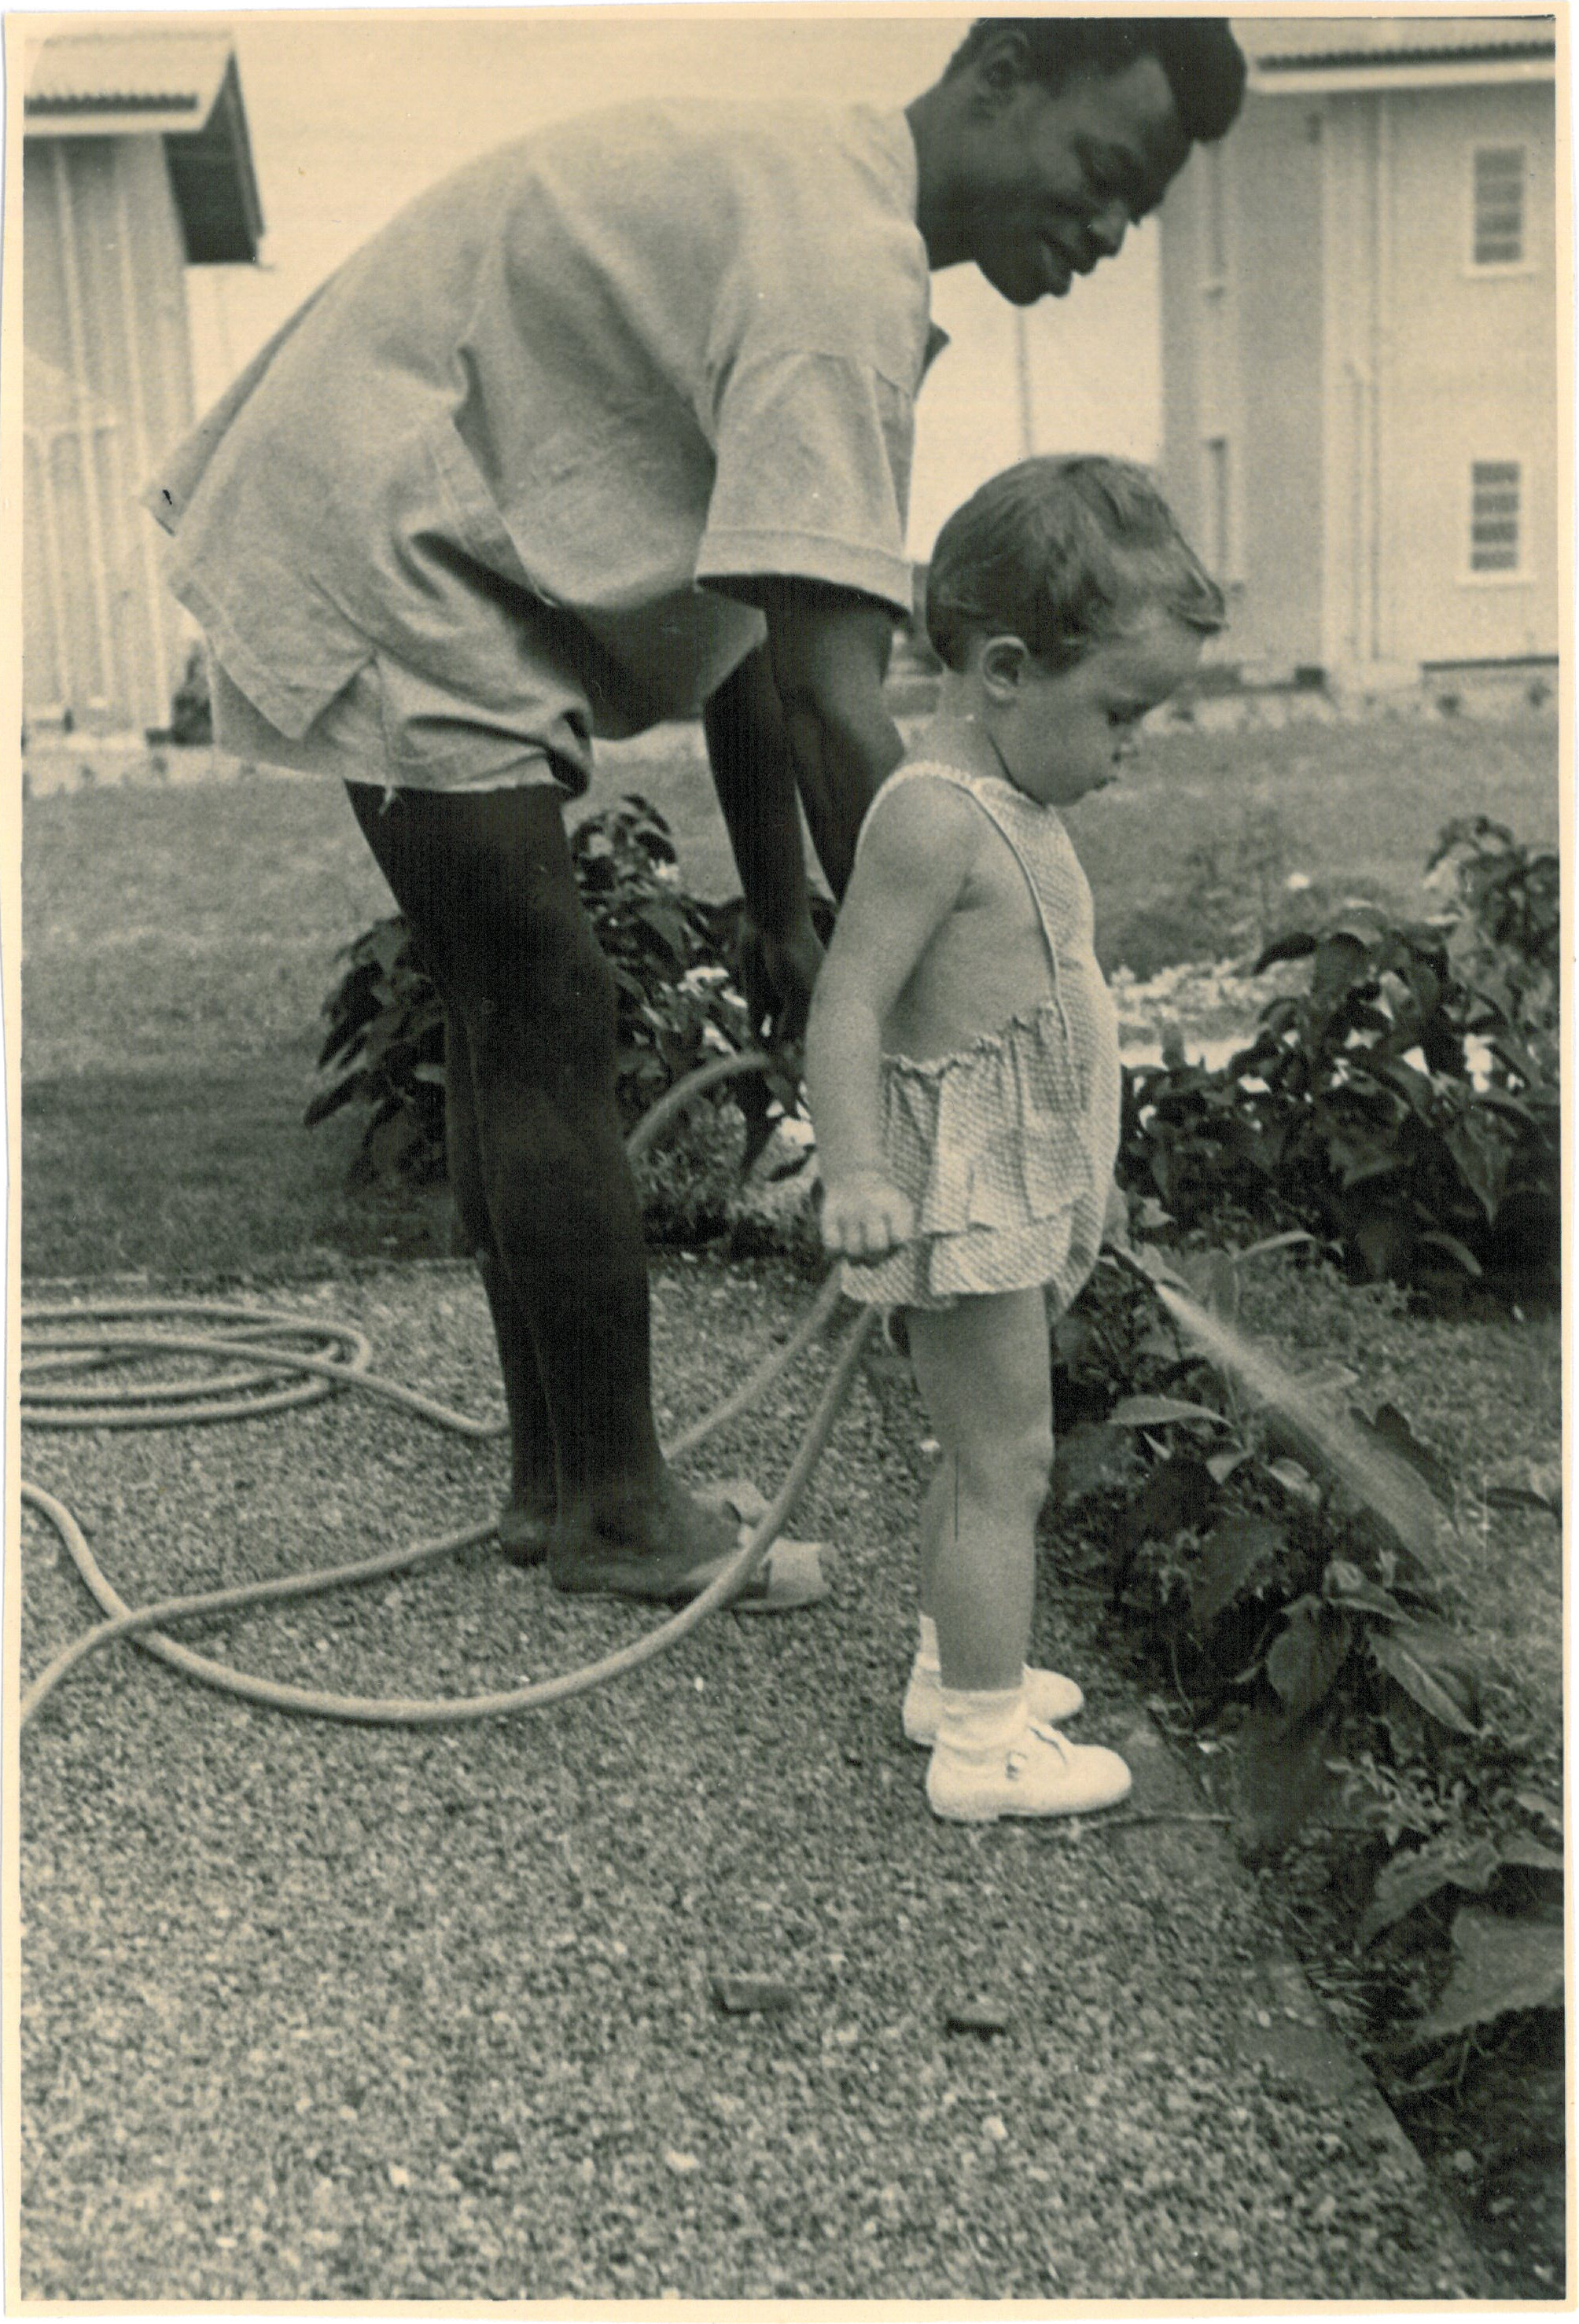
\includegraphics[width=0.45\textwidth]{photos/elizabeth-with-gardener.jpg}
    \label{elizabeth-with-gardener}
  }
  \caption{Elizabeth with (left) Audu and (right) Andrew (Lagos,
    1962).}
\end{figure}

There was a large expatriate community in Lagos and we made many
friends, particularly, in my case, of women. I became a colonial wife;
there were countless tea and coffee parties and we would vie with each
other to produce the biggest variety of cakes etc. How silly! But it
helped to pass the time! I smoked in those days too, to be social. How
very silly!

I did a lot of sewing in those days and I would be at the sewing
machine by 8~am, until Elizabeth came home from school (our chauffeur
would take her). I can hardly believe that I did not get out of bed
before 8~am, by which time Tony had had his breakfast and gone to
work.

My hobbies have always been of the needlework variety -- sewing,
knitting, embroidery, dressmaking, etc. My first attempt at embroidery
was of a bunch of daffodils on a tray cloth. In the making I took it
with me when I went to stay with my grandmother. I think I was about
twelve. I was ``caught'' working on it on a Sunday morning and I was
in real trouble. Sewing in the morning when there are jobs to be done
and on a Sunday too! Whatever next?!

I must have learned the basics of sewing at school and I knitted
during college days but it was not until we got to Nigeria that I
started to sew ``seriously''. I found a hundred-year-old Singer sewing
machine waiting for me when I arrived in Lagos with Elizabeth. Tony
had acquired it (I thought you might like to make curtains for the
house. Goodness! Full-length and lined -- a learning curve indeed!)

I had to cut the curtain out on the floor because of their size and
the iron was handy. We were very amused when Elizabeth told Grandpa
that she had to be careful not to burn her ``botham'' (bosom).

The machine did wonders for me and it was thoroughly used to make
clothes for the children and myself. It is likely to survive several
more hundred years because of its unique sturdiness.

Being a ``colonial'' wife I had time on my hands and I started to sew
at 9am! Clothes for Elizabeth, Richard, and myself. My great joy was
to make something out of something else -- my triumph was four
maternity smocks out of two dresses; and a friend gave me eight
cast-off dresses of her daughters for me to alter and make dresses for
Elizabeth. Which turned out very well indeed. Also I used Tony's
discarded white ``sea-island'' cotton shirts to make shirts for
Richard -- wonderful material -- and, by placing the pattern so that
the existing button-holes were in the right place, the finished
article managed to look professional!

``Make do and mend'' was a slogan we learned during the war and has
always stayed with me -- although I think I probably inherited my
thrifty ways from Grandmother.

I loved mending and I even managed to be complimented by my
mother-in-law on my darning of Tony's socks! I mended a lot of
Elizabeth's childrens' clothes, even toys, and got a great kick out of
that. By the way, the sewing machine stayed with me and saw more years
of sewing in South Africa until I finally gave it away to the maid of
a friend who thought she had inherited the crown jewels!

I once went to Bristol after finishing college and saw a table cloth
in a needlework shop window. It was made of Irish linen and huge
transfers were in place. There was, obviously, a lot of work to be
done. This was the reason it had been reduced in price (its original
price was 29/11 and down to 9/11). I had to have it.

I only started work on it when we were in Turkey and it took me a
whole year to finish. It helped me through many long hours of being
alone and waiting for Tony to come back from work -- such rewarding
work. It has been used (and laundered. Oh my! What a task). I have
passed it on to Elizabeth and I hope it will be used. It is something
of an heirloom and I have embroidered my name and the date in the hem.

Audu would do the routine cooking and laundry work -- and Edward the
cleaning -- and so my mornings were taken up with sewing, coffee
parties and my special ``Goodies'' for lunch and dinner parties
etc. How this was to change when we got to Johannesburg and I had no
servants by choice. But that was to be 11 years in the future and life
in Nigereia was there to be enjoyed, sometimes hated and found to be
frustrating but nonetheless part of ``Life's Tapestry''. I had to go
back to Engalnd to have Richard in 1964 and we were delighted because
he now completed the family. Elizabeth was the perfect 4-year-old
mother and looked after him when I had to go out -- of course, Audu
was always there at these times. Things could get out of hand. If
Elizabeth tried to change a nappy, it would finish up around Richard's
ankles and once, when he was thirsty, she gave him lime juice which
had disastrous consequences! But both children brought us much joy and
we were very blessed.

In 1966, the Biafran war started and this brought some unpleasant
experiences. The state of Biafra wanted to break away from the Federal
Government and took up arms to support their cause. Differences in
Lagos were strong but people would try and live normally. We would
drive to dinner parties leaving the children with Audu -- an excellent
baby-sitter -- and be stopped on the road by a soldier -- either drunk
or drugged -- and Tony would be questioned about whether he was
carrying weapons etc., and we would both be frightened by the
demeanour of the soldier. ``Please God, let us get back to our kids''
I would pray silently.

In 1966 we had a first-hand share of the war. Tony had to go to Ghana
for just one night and that was the ``Night of the Aeroplane.'' Eleven
of the Biafran rebels hijacked a ``Fokker Friendship''
aircraft,\footnote{The Fokker F27 Friendship 5N-AAV operated by
  Nigerian Airways was hijacked on October 7, 1967, while \textit{en
    route} from Benin to Lagos. See
  \href{http://www.mercenary-wars.net/biafra/index.html}{http://www.mercenary-wars.net/biafra/index.html}
  and
  \href{http://news.google.com/newspapers?nid=1774&dat=19671007&id=Pn4fAAAAIBAJ&sjid=6mUEAAAAIBAJ&pg=7328,1581485}{Picture~\ref{hijacking}}.
} loaded it with dustbins filled with explosives, and flew to Lagos in
the hope, it was thought, of blowing up the home of the president
(Jacobu Gowan) and government buildings. Something must have gone
sadly wrong because, instead of the dustbins being pushed out of the
plane, they blew up in mid air -- immediately above our house as it
happened. The children were with me in our bedroom and the bottom fell
out of Richards cot which landed him on the floor. He looked at me as
if to say ``What the devil is going on?'' The noise of the explosion
was terrific and I was more terrified than at any time during the
second world war. Small pieces of the plane were falling on the roof
and sounded like fire -- I was convinced that we were
trapped. However, we got downstairs and neighbours called. Windows had
been blown out and there was glass everywhere. I forgot to put on a
dressing gown but it didn’t worry me that Wally, our Australian
neighbor, showed a particular interest in me and my flimsy nightie!
There were body parts scattered over the garden and Wally found what
he thought was a flying glove but was actually a complete Negro scalp!
We made tea (of course).

\begin{figure}
  \centering
  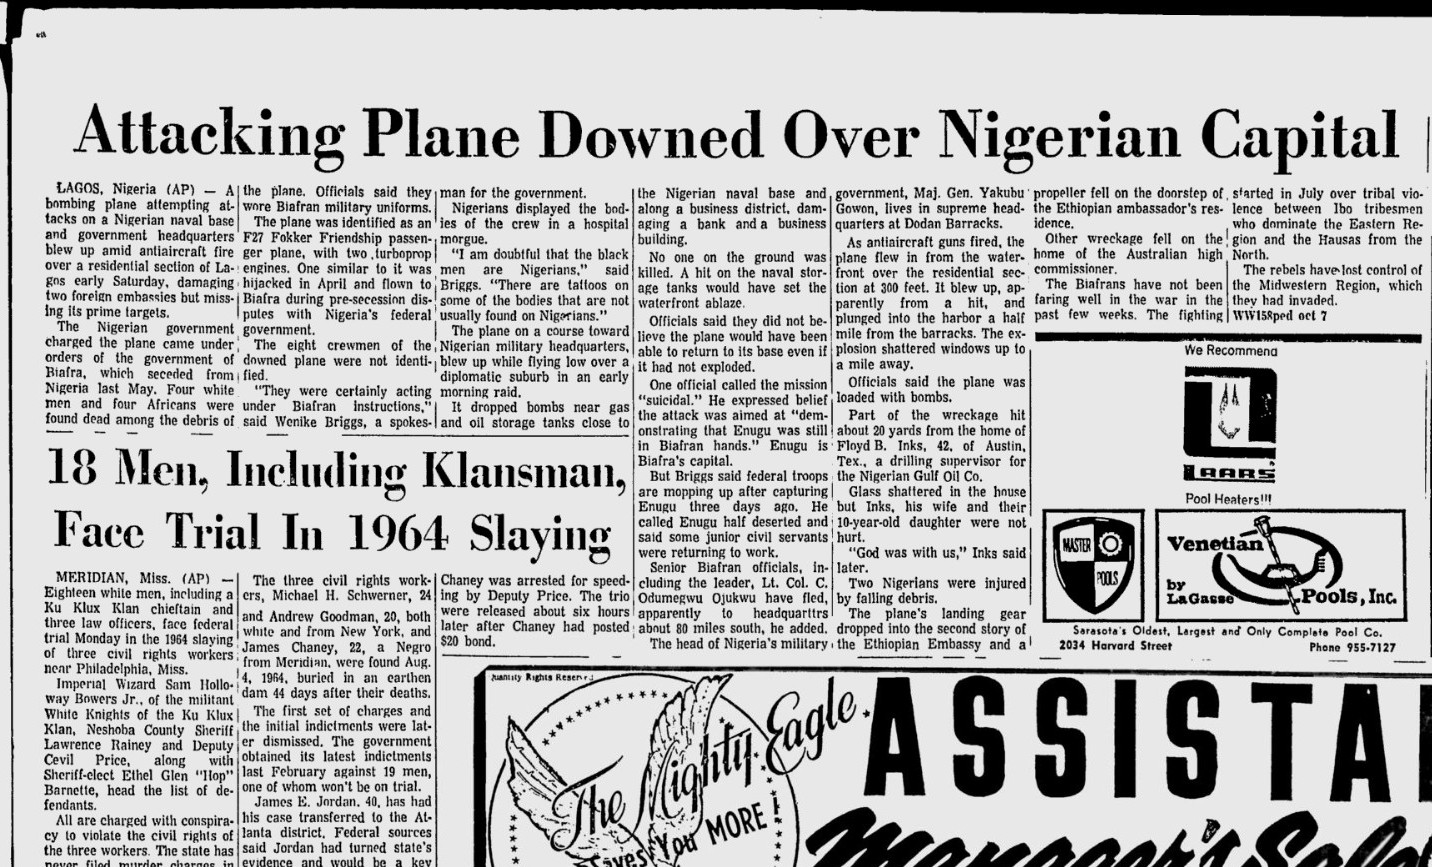
\includegraphics[width=\textwidth]{photos/nigeria1.jpg}
  \caption{From the October 7th, 1967 edition of the Sarasota
    Herald-Tribune.}
  \label{hijacking}
\end{figure}

We went back to bed but sleep was impossible, the morning light
brought sights to behold with brains hanging on bushes and complete
chaos. But that could have been much worse for the plane itself had
crashed into the creek. However, one of the doors had slid down the
side of our house and part of a wing had come through the roof. It was
raining so that made things rather inconvenient! Another wing had come
through the Weber's roof and landed on Nicola's bed. She would have
been killed if she had not gone to England with her mother the day
before. Her father (Ogy) had been to a party and got rather
drunk. When he came out of his bedroom and saw an arm and a hand on
the stairs he thought ``My God, I had more to drink than I thought I
had!'' But nobody was hurt which was a miracle. Tony returned to find
utter mess and chaos and it was only then that I gave way and burst
into tears. I had to have a course of vitamin B12 injections to get
over the trauma but things came right and somehow a sense of humor
persists and one is able to see the funny side of things
eventually. However it was not amusing for the director of the P~\&~T
to say to Tony ``A disaster to your family would have been no more
than you deserve.''

How racism rears its ugly head.

The Biafran rebels gained nothing from this escapade and I am not sure
if they ever managed to break away and gain their independence. There
were some in Nigeria (Nigerians) who said that Britain should never
have given that country its independence and I am of the belief that
most African countries have fallen flat on their faces and elected the
most incredibly awful, greedy, and incompetent leaders. I write this
in 2011 when we are witnessing the downfall of Egypt, Syria, and Libya
and starvation in Kenya and Somalia. But my thoughts are still in
Nigeria where we stayed for 11 years and we had a good life in spite
of the Biafran war. Luckily we had efficient guardian angels and I do
believe that I have had an army of guardian angels watching over me
throughout my life.

The memory of one will always be with me.

One day in 1966, when we were living in Lagos, I was persuaded,
against my better judgement, to spend the morning on a beach with
three of my friends and our combined number of 7 children. Elizabeth
was 6 and Richard 2. The beach was notoriously dangerous for having
claimed lives and, indeed, whole villages over a period of time. But,
nevertheless, it was a calm morning and not too hot. The two
Australian sons of our neighbours went into the sea and took Elizabeth
with them. All was well until a rogue wave came up to the shallows and
took the three kids out 6 feet. The boys' Australian mother, a strong
swimmer, went in to fetch them and I went in to fetch Elizabeth, which
was madness, as I can't swim -- even though I was born under the sign
of Cancer, a water sign. But I had to get my child -- there is nothing
as strong as the umbilical cord -- so there were now two of us
stranded in a restless sea. And then there appeared a man -- a
Nigerian -- dressed in the purest of white robes holding out a hand to
each of us. The sea parted and so he drew us to safety. The experience
must have lasted for 10 seconds but it seemed a lifetime.

Having drawn breath and being in the safety of the beach, I asked my
friends where that man had gone. But they denied any existence of such
a man ``No, Madge, there was no man here. You just walked out of the
sea.'' And it was useless to argue with them. We had been rescued by a
black man in the most dazzling of white robes -- beautiful to behold
-- my everlasting memory is of a guardian angel.

Thanks be to God.

Whilst we were in Nigeria (approximately 1970), cholera became endemic
and it is surprising that the disease had not gripped the country long
before -- perhaps it had but without World Health Organization
publicity.

Hygiene is a necessity in 3rd world countries but when a family has to
share a bucket of water (obtained with difficulty) it is not
surprising that such a disease can be easily transmitted.

Deaths occur because of severe dehydration. Once more we had to submit
to more injections and anyone coming into our house was ``invited'' to
wash their hands at the kitchen entrance. I checked up on Africans
through a peephole and called them to wash their hands if they had not
done so!

Once more, we were able to resist infection; in fact we had not
succumbed to other diseases there such as malaria, which is still
prevalent in the world.

Public executions for crimes such as murder, or even armed robbery,
were quite common and witnessing these events was very popular. And a
``day out'' with lots of excitement was very much welcomed by
thousands of people -- rather like going to the races. A popular venue
was close to our house and we could not help seeing the hordes
arriving; there was much excitement. We understood that refreshments
were available! Faintly we heard the gunshots ring out -- criminals
were strapped to fuel drums. Oh! It was horrible, but capital
punishment (perhaps administered more delicately) is necessary I
believe, and I can never see the point of keeping a violent criminal
alive to enjoy the comforts of a modern prison.


\chapter{South Africa}

Our lives in Nigeria continued until Tony accepted a position with the
GEC in South Africa. A year before we moved Elizabeth had reached the
age of 12 when there was no more schooling in Lagos and so she had to
go to boarding school in England (Wroxall Abbey). She was looked after
by Mandy Price who also attended the school and was the daughter of
Tony's boss Mel Price. We stayed with Mel and Audrey until the time
came to take the girls to school. My only thoughts on this day was
that Elizabeth would be away from us and in a different country. My
heart was heavy when we left her but there were no tears until bed
time when Tony said ``I was very proud of you today.'' I think my
heart burst and my tears soaked my pillow. Fortunately she was able to
fly out to us during the year and became a seasoned and confident
traveler. But oh! How she was missed.

Well we had our 11 years in Nigeria with its ``ups and downs'' and
good and bad memories.

What a difference to leave black South Africa and arrive in what I
called white South Africa. Of course the hideous apartheid regime was
in full force and life was terrible for the blacks who were deprived
of so many things, but the days were sunny and life seemed to have an
air of well-being. Tony made several trips to South Africa before
leaving Lagos and it was hard to believe that life was so good. It
almost seemed to him that ‘our’ blacks had been worse treated. For
instance, while the servants in South Africa were well fed and looked
after, the servants in Nigeria had to fend for themselves more and --
in line with other households -- the only food we gave to Audu and
Edward (apart from the odd ``handouts'' of cake etc.) were a leg each
from the turkey at Christmas and a bottle of beer! And once at a
dinner party, the hostess excused herself in order to take her cook
home. In Nigeria, servants had to walk miles to and from work. Our
gardner walked 6 miles to and from our house every day.

From being a colonial wife, I turned to being a conventional housewife
in Johannesburg. For one thing the climate was fabulous (best in the
world some say) and much easier to cope with everyday events rather
than having to fight against low energy and frustration in the
debilitating Lagos atmosphere.

I have never been very artistic and failed miserably in the art class
at school so it was something of a surprise for me to become
interested in cake icing -- which is actually an art form today. Cake
decorating was destined to become simpler and less time-consuming than
it was when I came to S.A.; that was when I became most interested.

I did, however, make our own wedding cake in 1953 and I cringe when I
see photos of it for it was far too elaborate and over-decorated and
looked like something Miss Havishan may have had for her aborted
wedding!

However, one learns and, after several years and help and
encouragement from a friend, Beryl Webb, I became really interested
and fascinated and managed to produce some acceptable
offerings. Luckily I had plenty of time. It was so worthwhile and I
found much satisfaction in giving the finished cake as a wedding
present.

I was told to be in the room before the bride came to see her cake for
it was the look on her face which told me her reaction. Luckily there
were no looks of complete horror!

It was worth every minute of the time spent making flower decorations
and, looking back, makes me feel glad to have taken up this hobby.

Not only wedding cakes took my time but I ``graduated'' to Christmas
cakes and, of course, cakes for the childrens' birthdays. Once, when
delivering Lisa's ``ballet'' cake, a nearby hedge grabbed the tulle
decoration and caused a complete fiasco. Lisa didn't seem to worry too
much.

Elizabeth and Richard had cakes for their 21st birthdays and Tony's
60th birthday one was ``interesting'' as he was interested in
astronomy. That was the theme. I put images of the planets round the
outside of the cake (see Picture~\ref{cake-astronomy}).

\begin{figure}
  \centering
  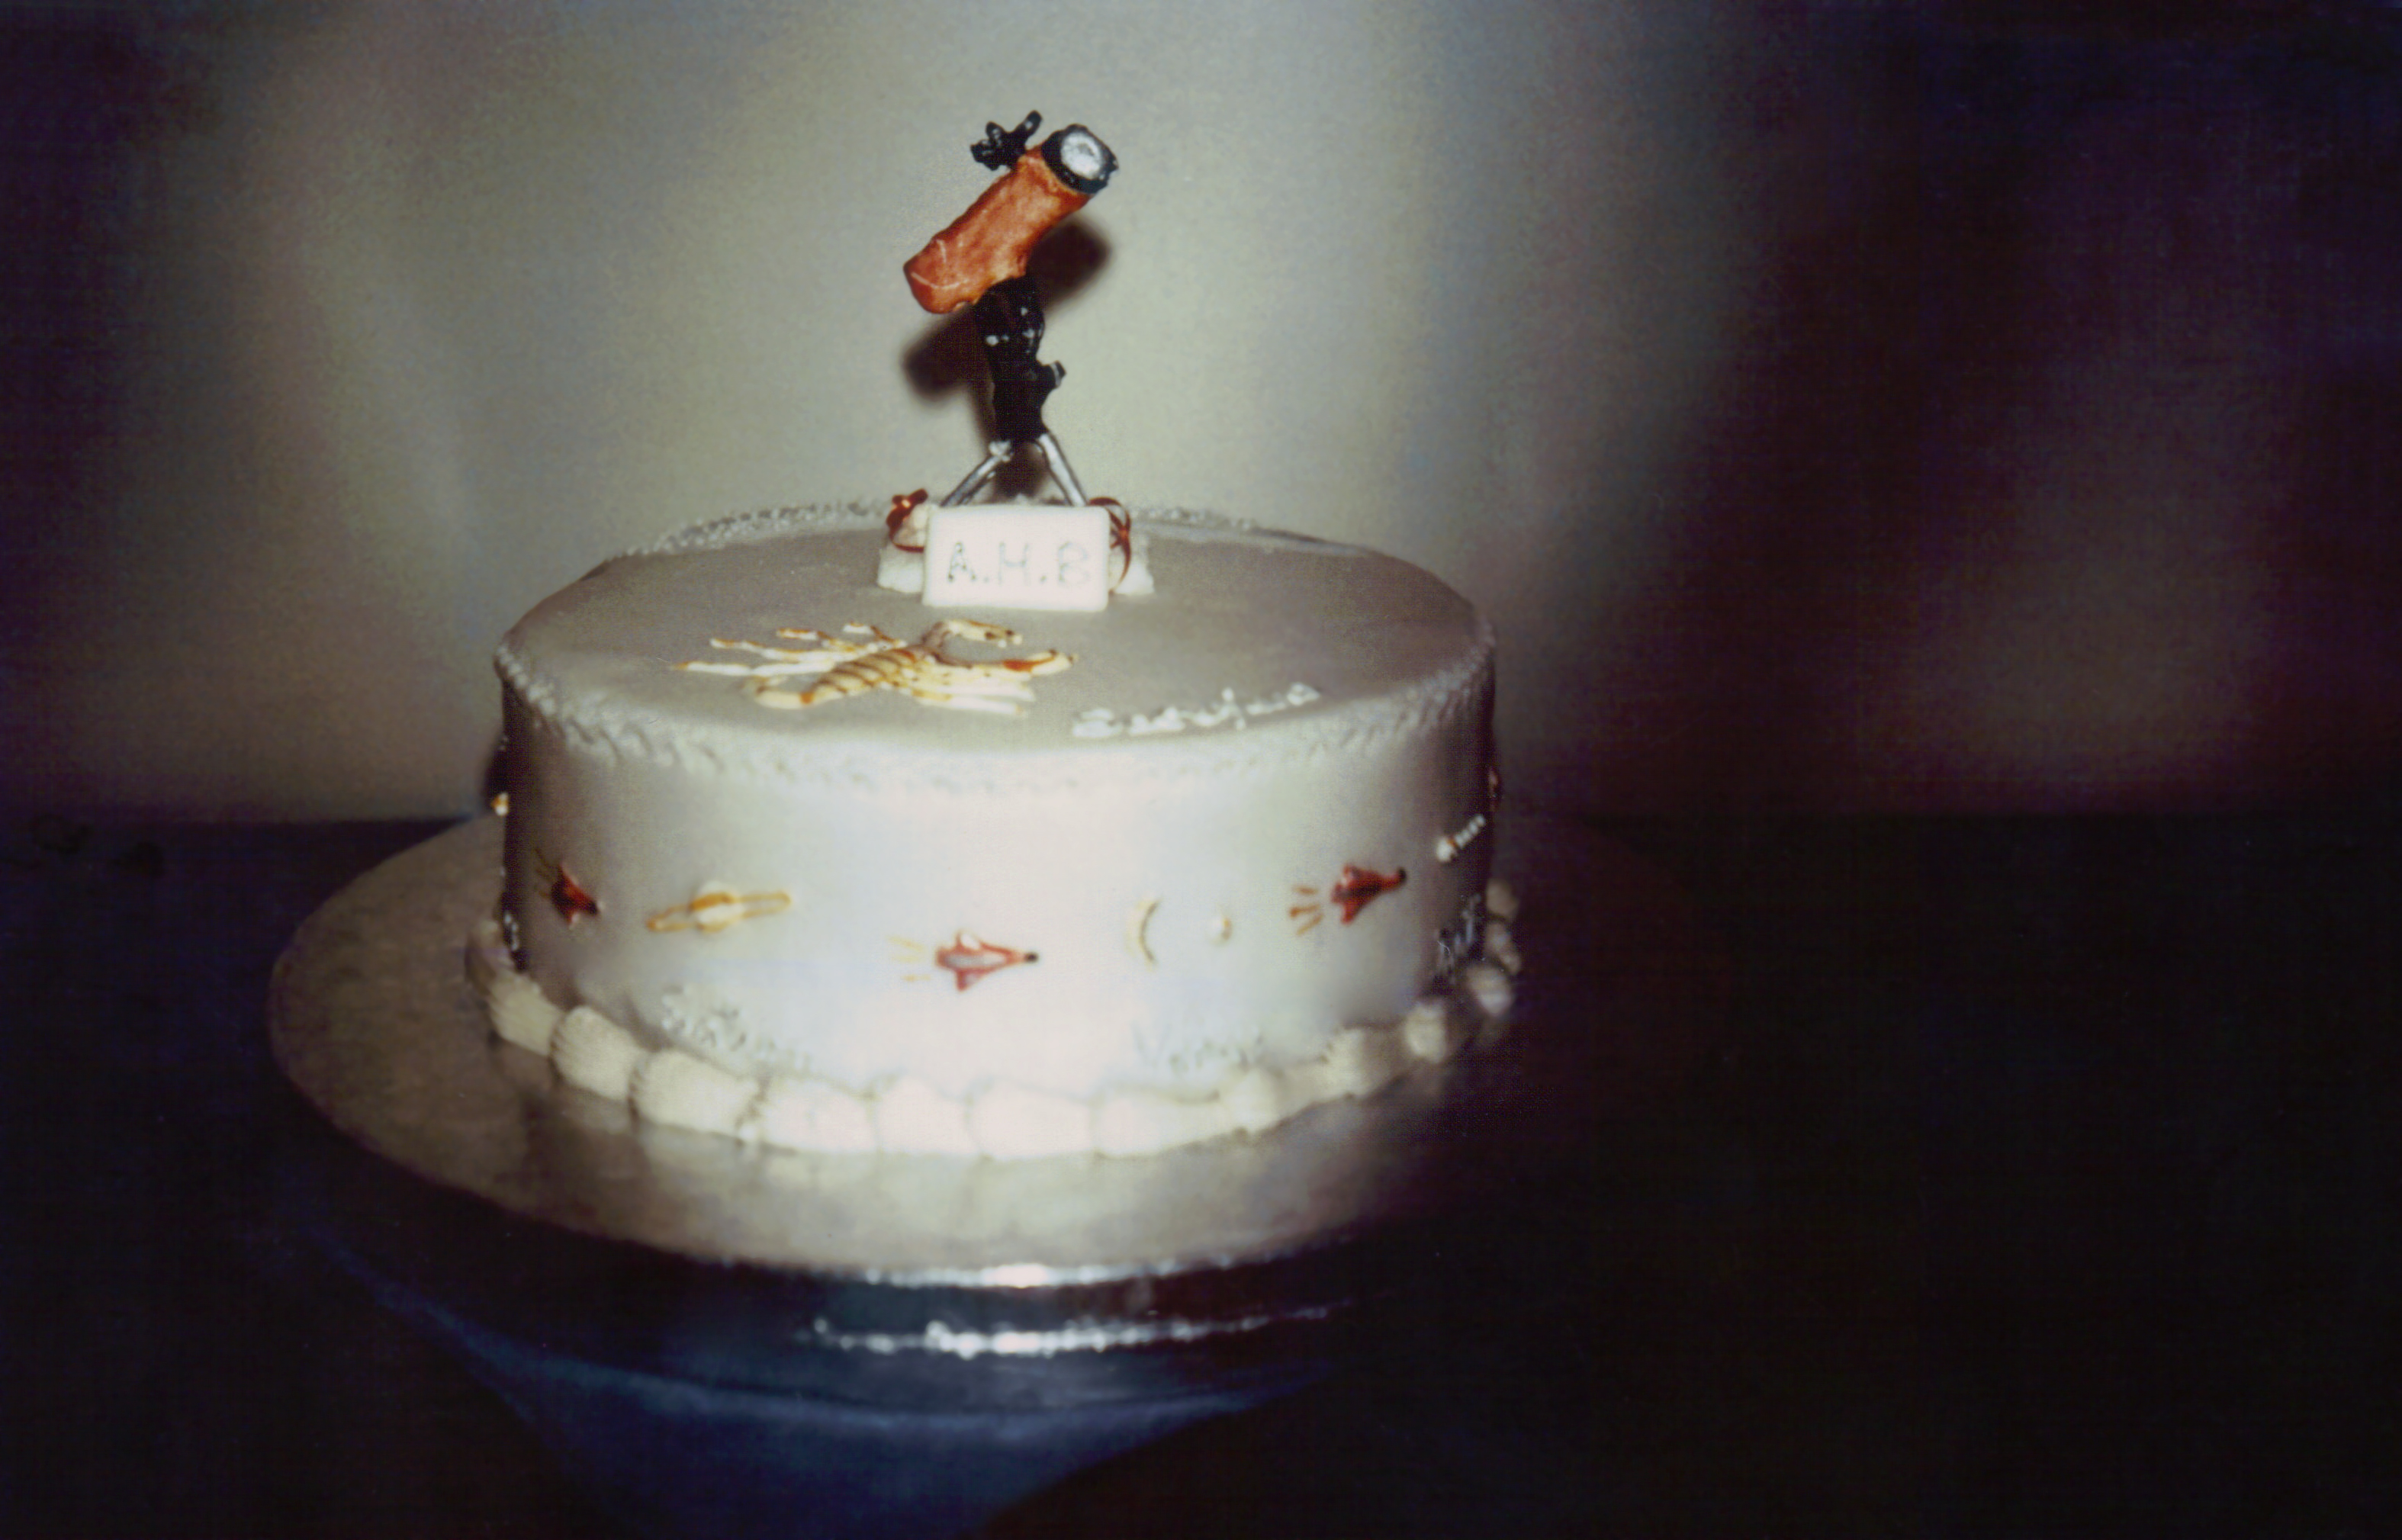
\includegraphics[width=0.9\textwidth]{photos/cake-astronomy.jpg}
  \caption{Tony's 60th birthday cake had an astronomy theme.}
  \label{cake-astronomy}
\end{figure}

I spend the whole of one day fashioning a telescope which was a
nightmare as the wretched thing kept falling over! However, it was OK
on the day and Tony was surprised and delighted. Crikey! I held my
breath!

We had to find somewhere to live and chose a location close to Phil
and Enid Hardisty -- Lombardy East -- the house was in need of repair
and I would be collected from our temporary home in a suburb of
Johannesburg by the man and his son who were to repair the house. I
was complete with bucket, mop, and apron, etc. and set about making it
more habitable.

One day he took a wrong turning and we found ourselves in Alexandra
township -- very, very black and awful. But there must have been
something of Nigeria left in me because I felt I had come home and
said ``this is more like it''! Both men thought I had gone mad!

We settled down to life in Johannesburg, South Africa. Elizabeth came
back to us from her English boarding school and went to Roedean. Where
she did well and obtained a good matric. Richard went to St. John's
college as a weekly boarder. He seemed very upset when we took him
back on Sunday evenings but he has said that he absolutely adored
being there. Just shows how one can get the wrong impression! Richard
also won his matric and settled down to a career in the hotel industry
and training first of all with Holiday Inn.

We had settled in the house in Lombardy East when we learned that the
house was to be auctioned to pay for debts incurred by the previous
owners. We protested of course. But, after much unpleasantness, we
moved to a flat in Corlett Drive which was lovely but had the
disadvantage of facing west and, in the Johannesburg summer, it was
not an ideal place to live.

%% Removed to reduce duplication in next paragraph:
% ; we finally found our ``resting place'', a
% house in Bryanston owned by the company and about to be vacated by an
% employee and his family who were returning to Australia. We acquired
% the house for a song and we also acquired a most wonderful dog. An
% alsatian (German Shepherd) for he had belonged to this family and they
% wanted to leave him behind -- so long as we promised to take good care
% of him.

Having been unlucky with the house and flat we first lived in in
Johannesburg we were pleased to find another house in Bryanston. It
was offered to us to buy at a low price (by the company, Barlow's) as
the occupants were leaving for Australia; they offered us their dog
after making sure we would give him a good home and we were to have
ten years of pleasure from this wonderful animal -- an intelligent,
handsome, and faithful german shepherd (see Picture~\ref{sherman}). I
was often alone all day and he would station himself outside the room
I was working in so that he was always on guard. Elizabeth trained him
well in obedience.

\begin{figure}
  \centering
  \begin{tabular}{cc}
    \subfloat[Sherman.]{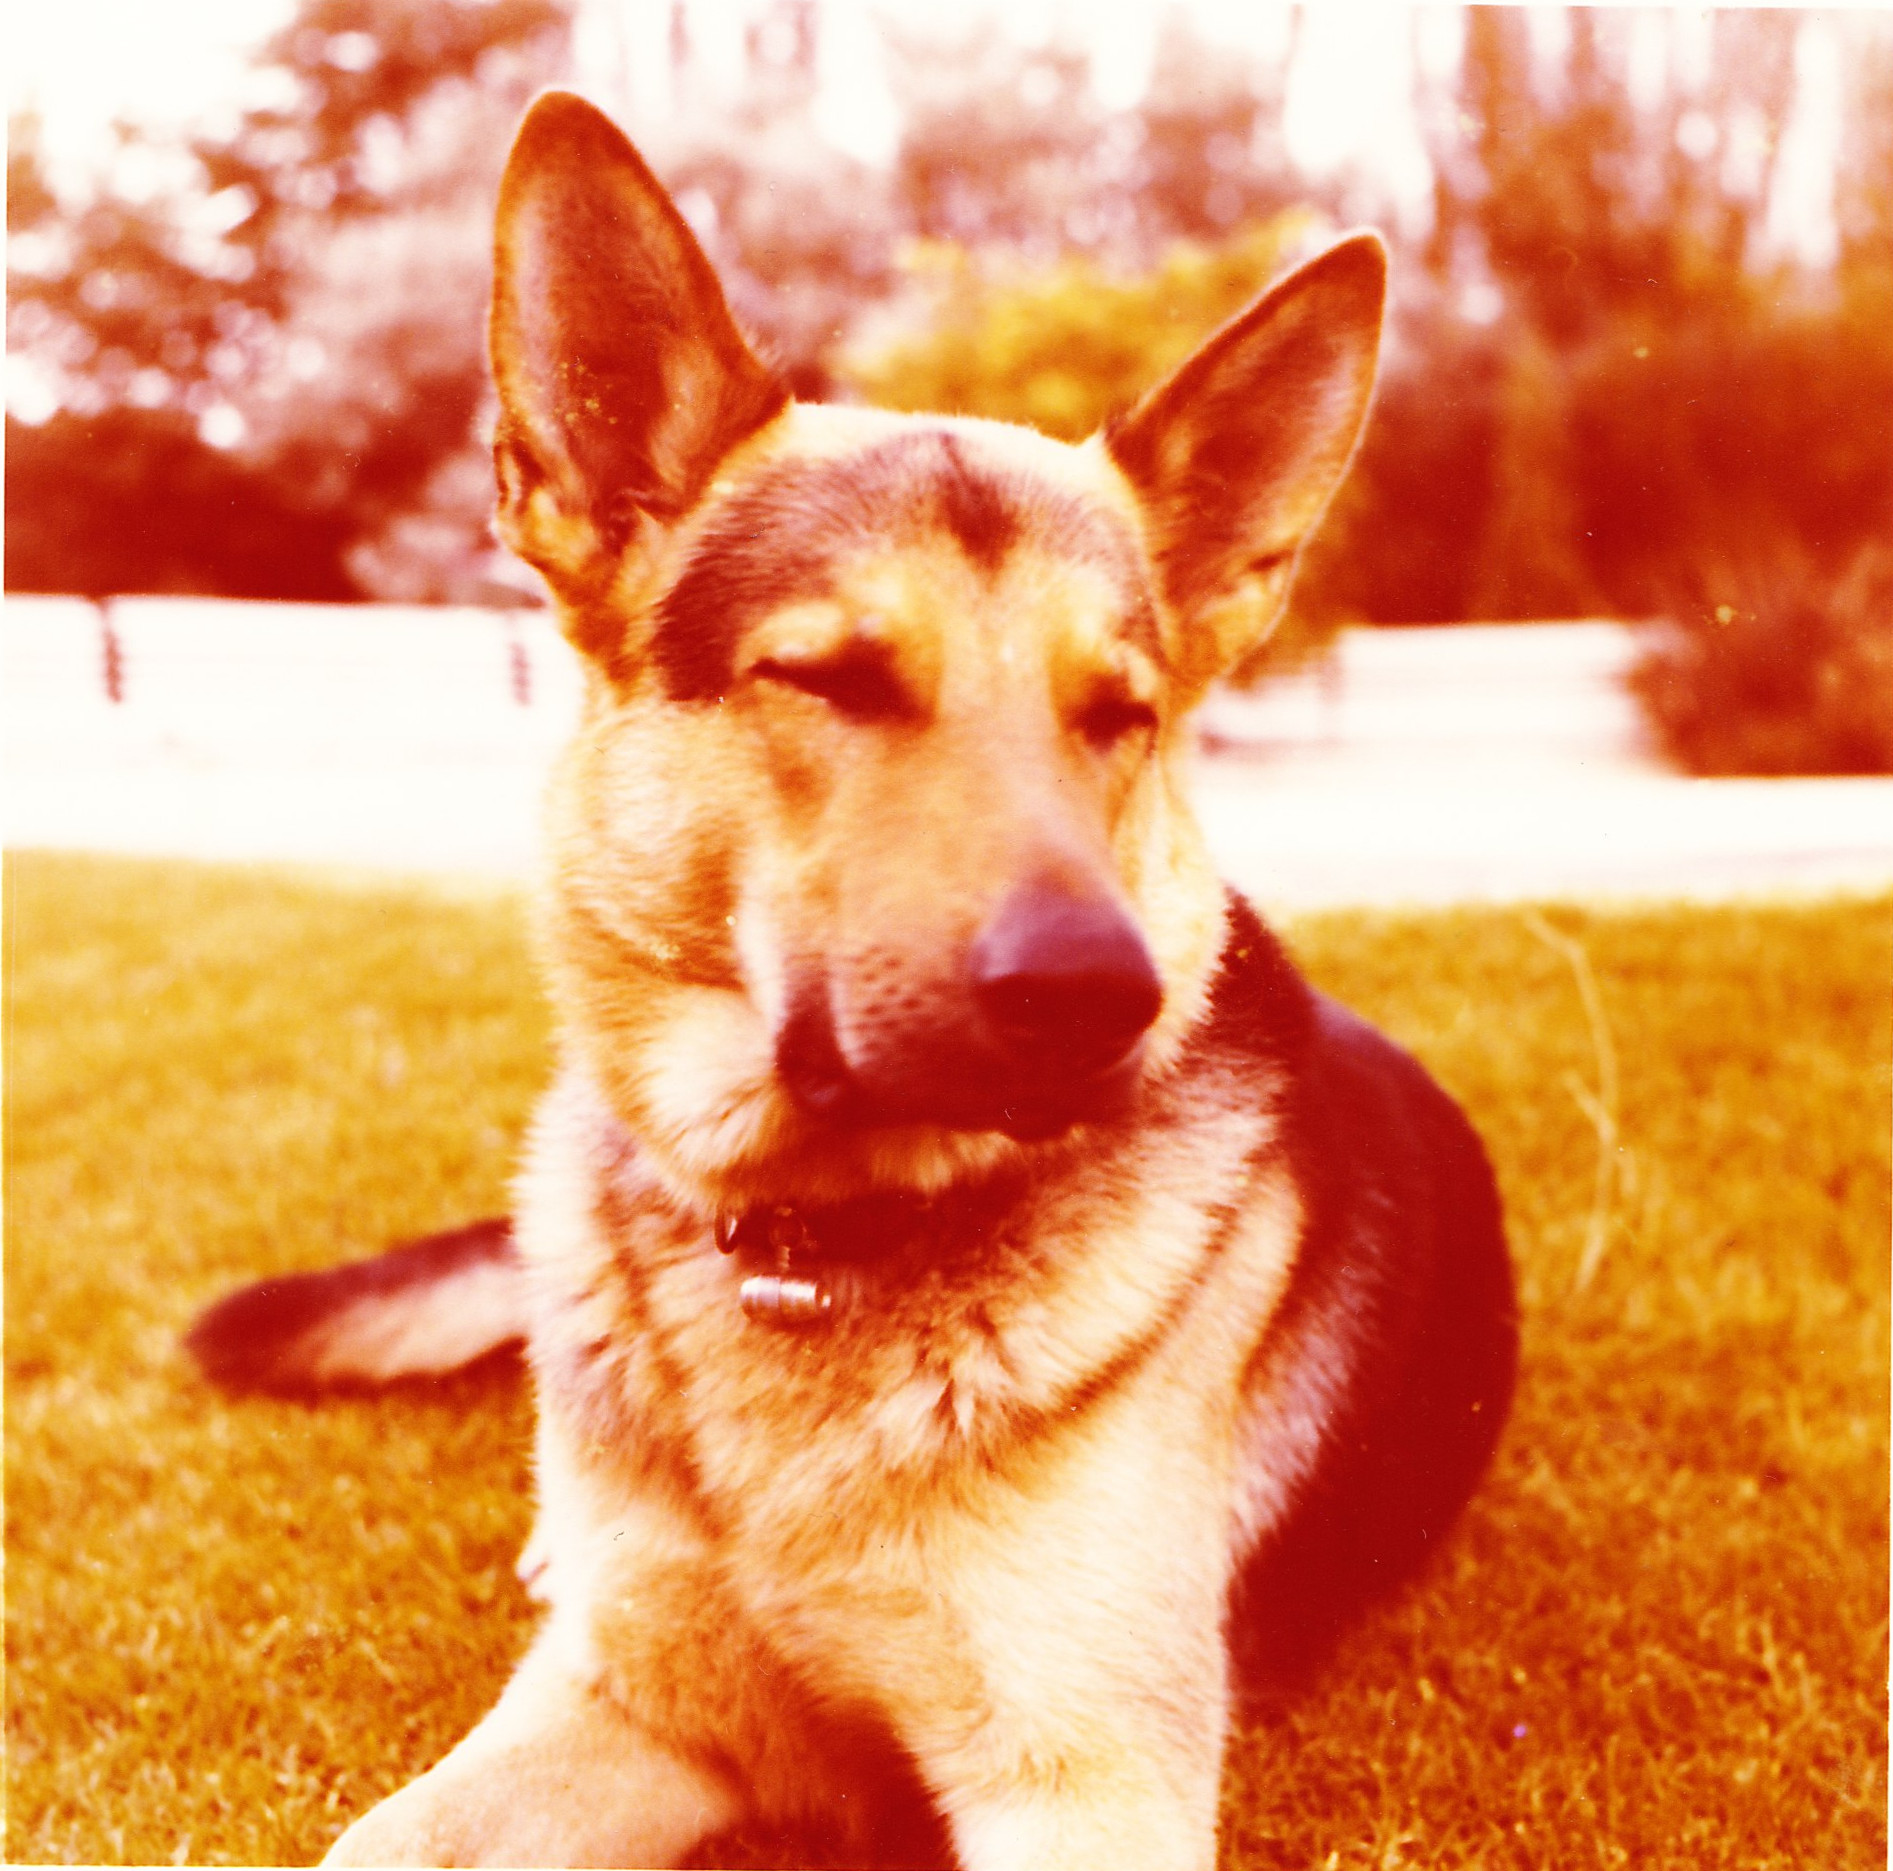
\includegraphics[width=0.45\textwidth]{photos/sherman.jpg}\label{sherman}}
    &
    \subfloat[Sydney.]{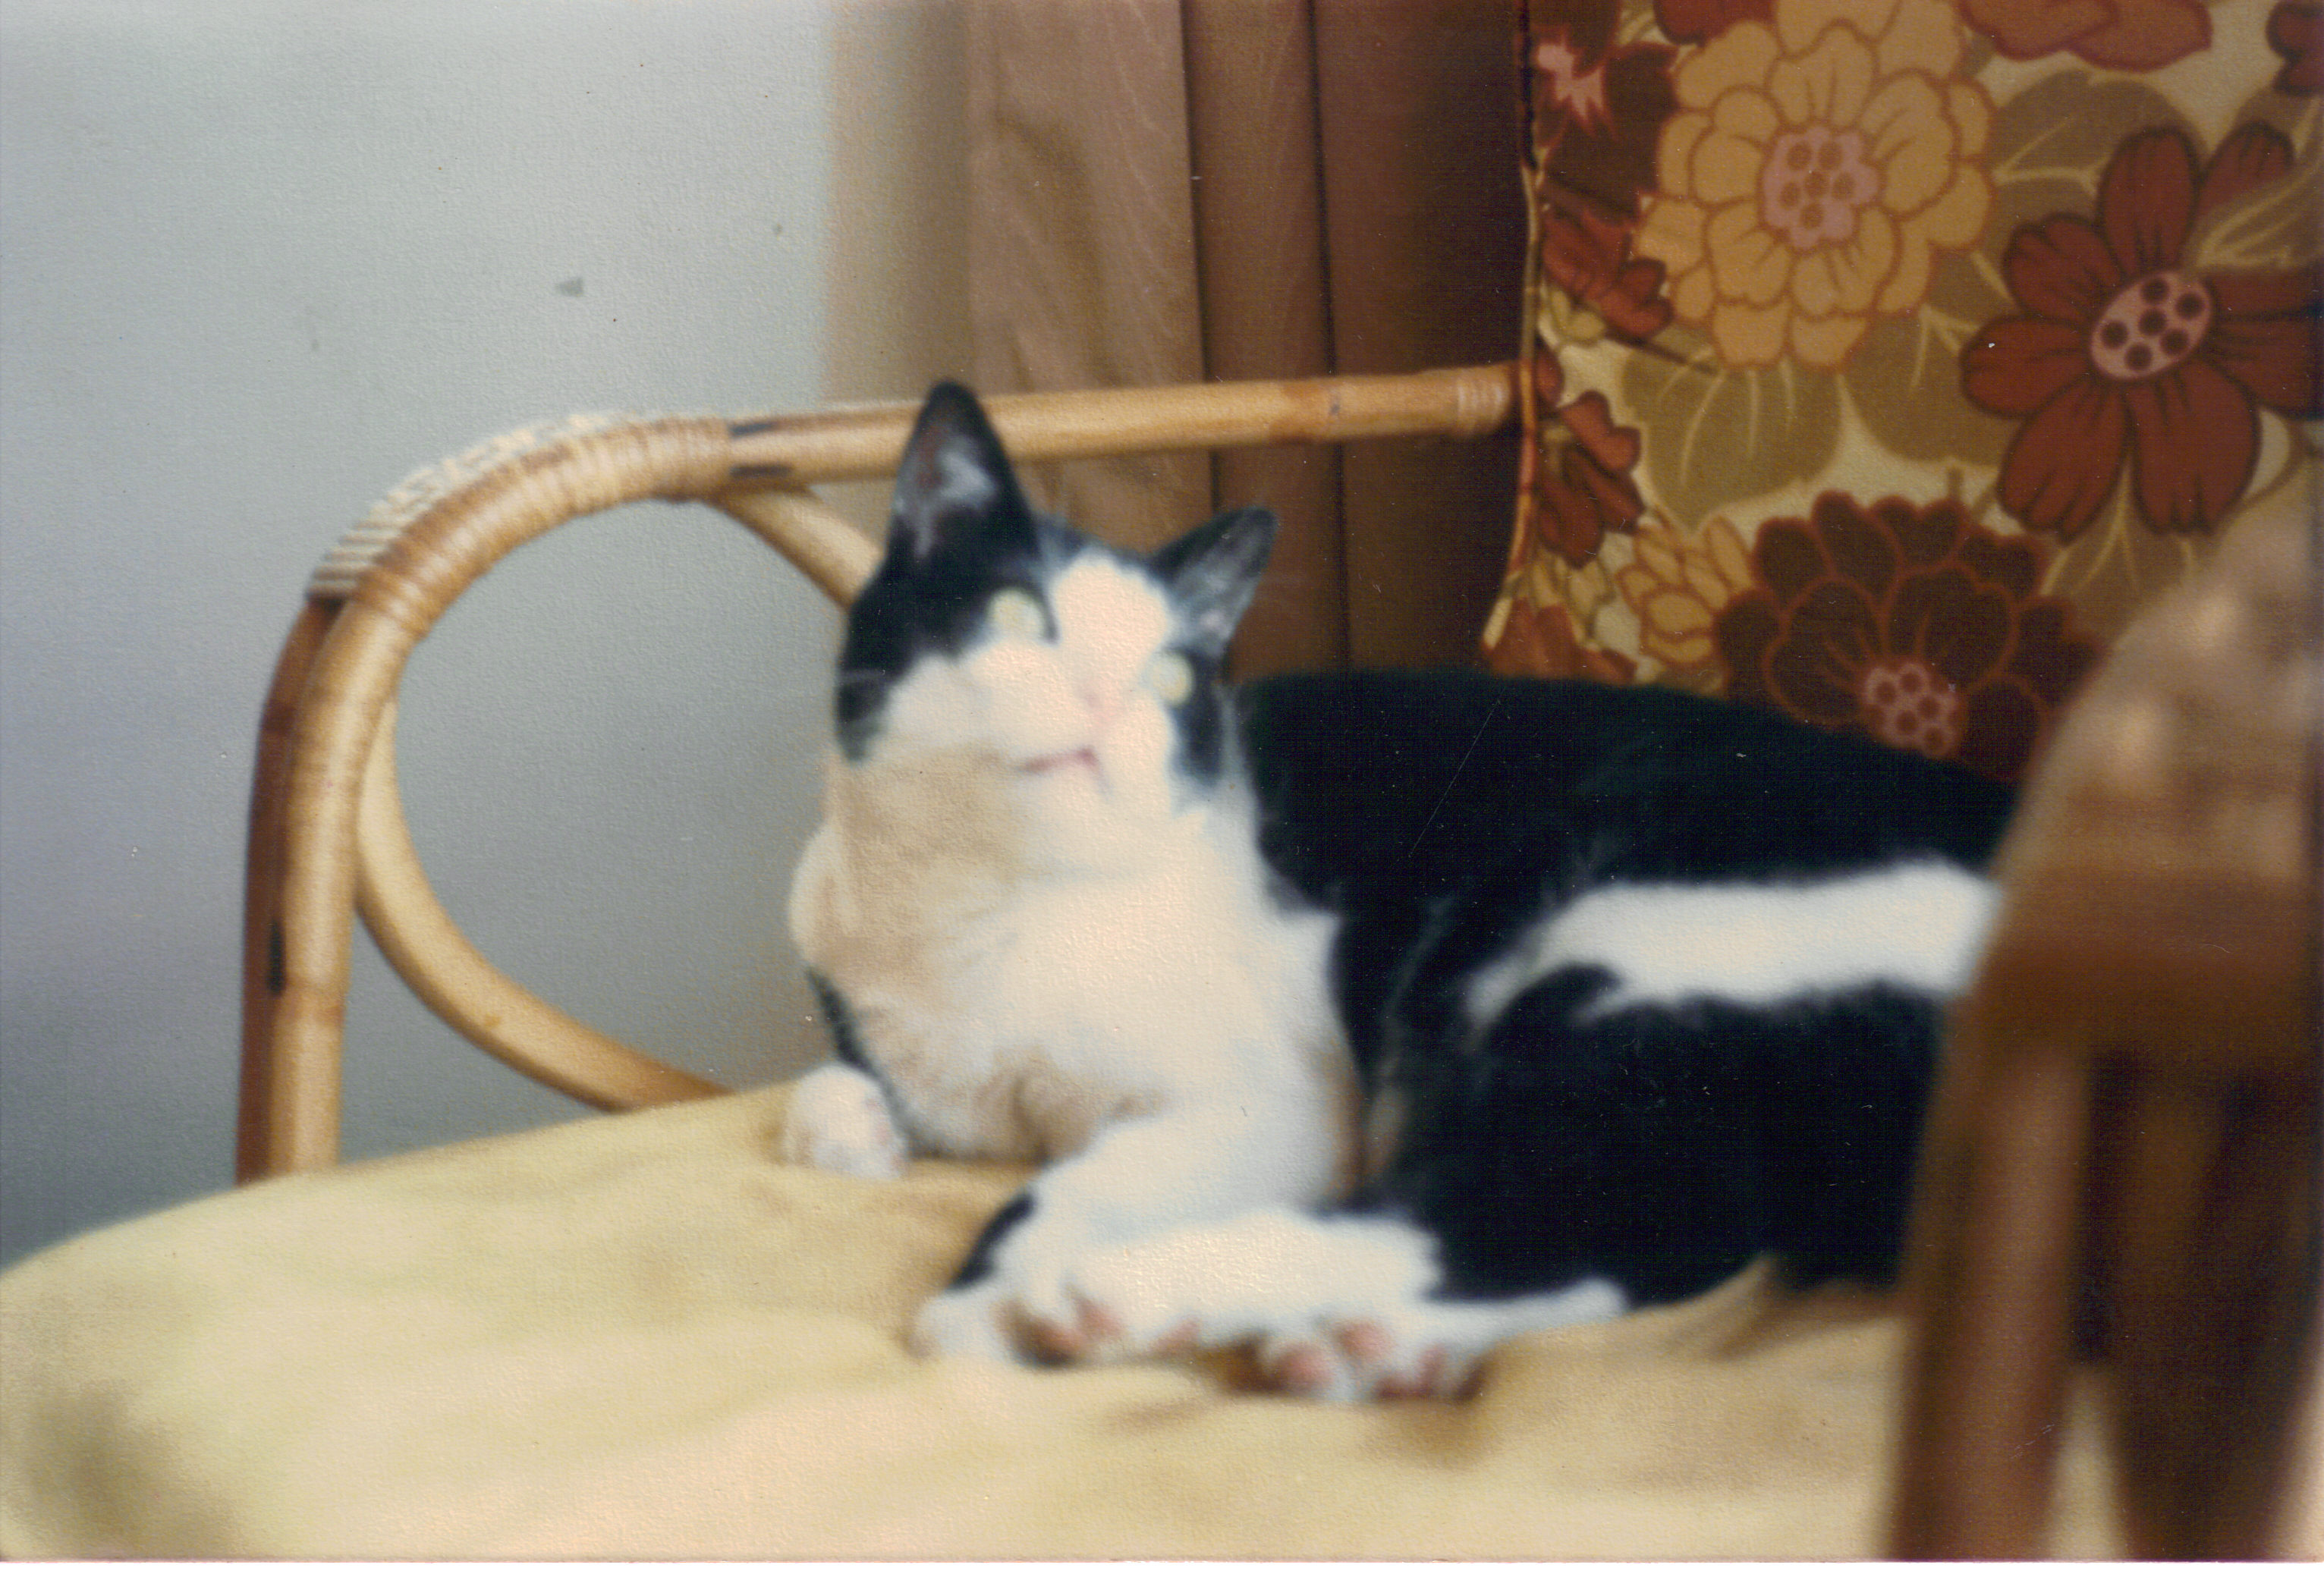
\includegraphics[width=0.45\textwidth]{photos/sydney.jpg}\label{sydney}}
    \\
  \end{tabular}
  \caption{Pets.}
\end{figure}

% \begin{figure}
%   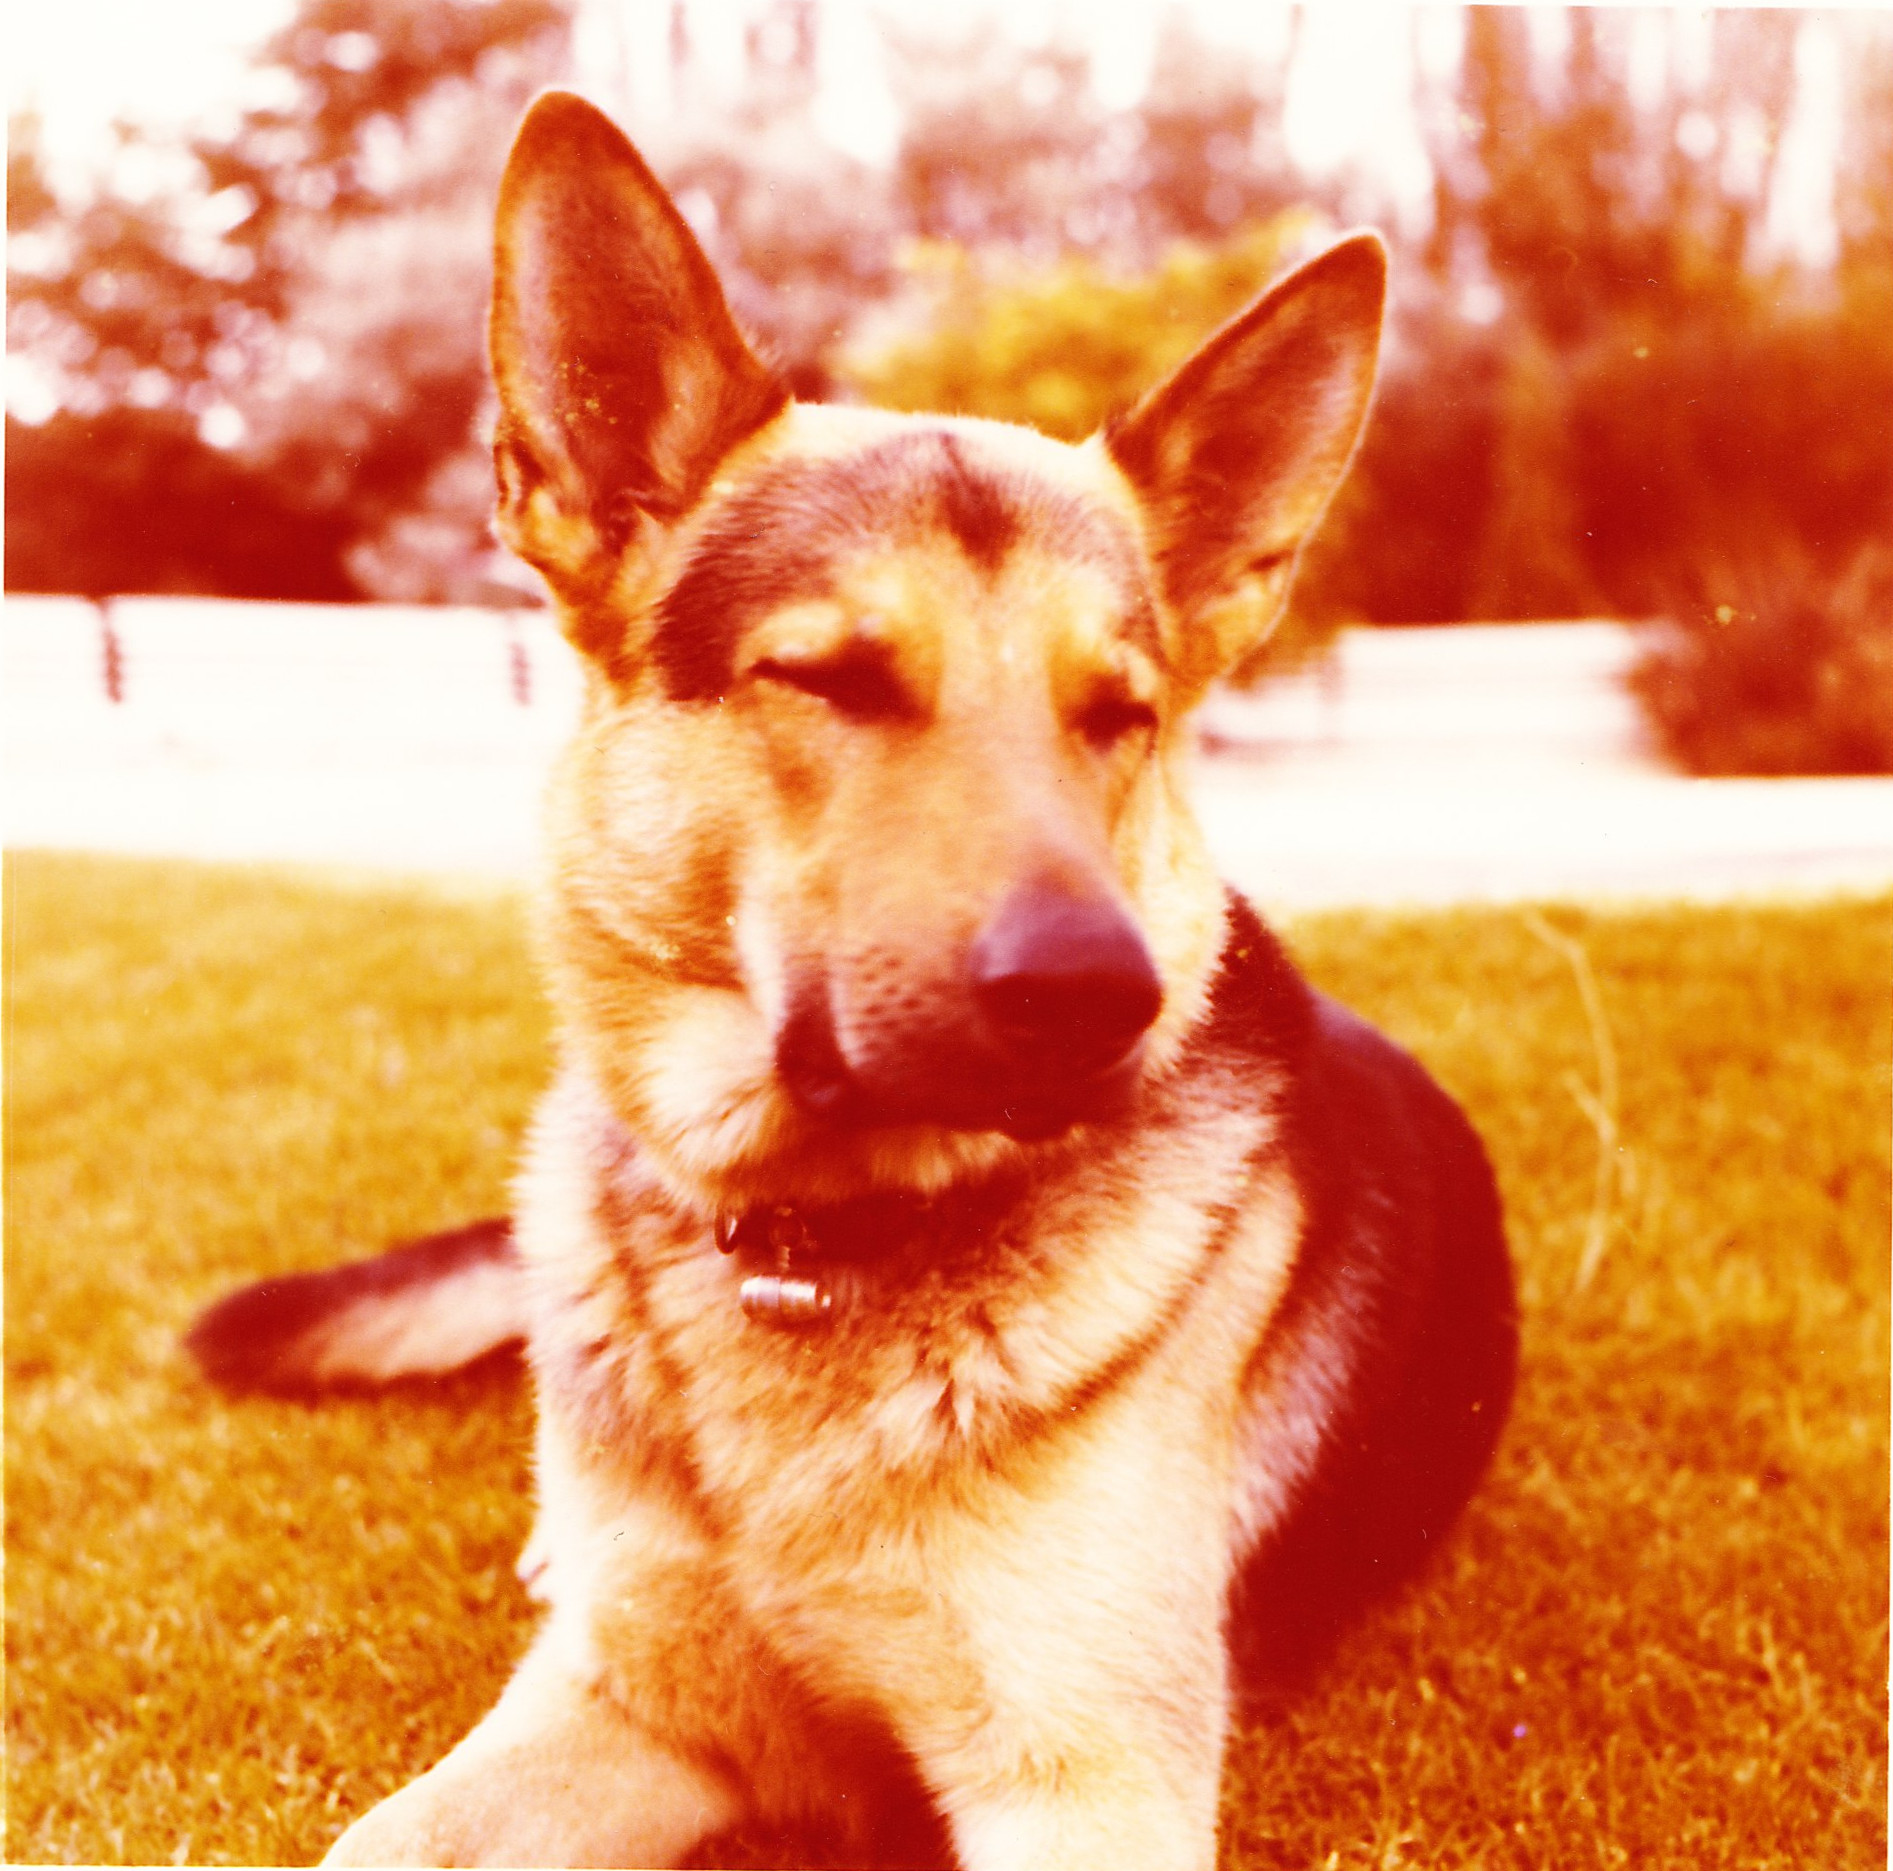
\includegraphics[width=\textwidth]{photos/sherman}
%   \caption{Sherman.}
%   \label{sherman}
% \end{figure}

% \begin{figure}
%   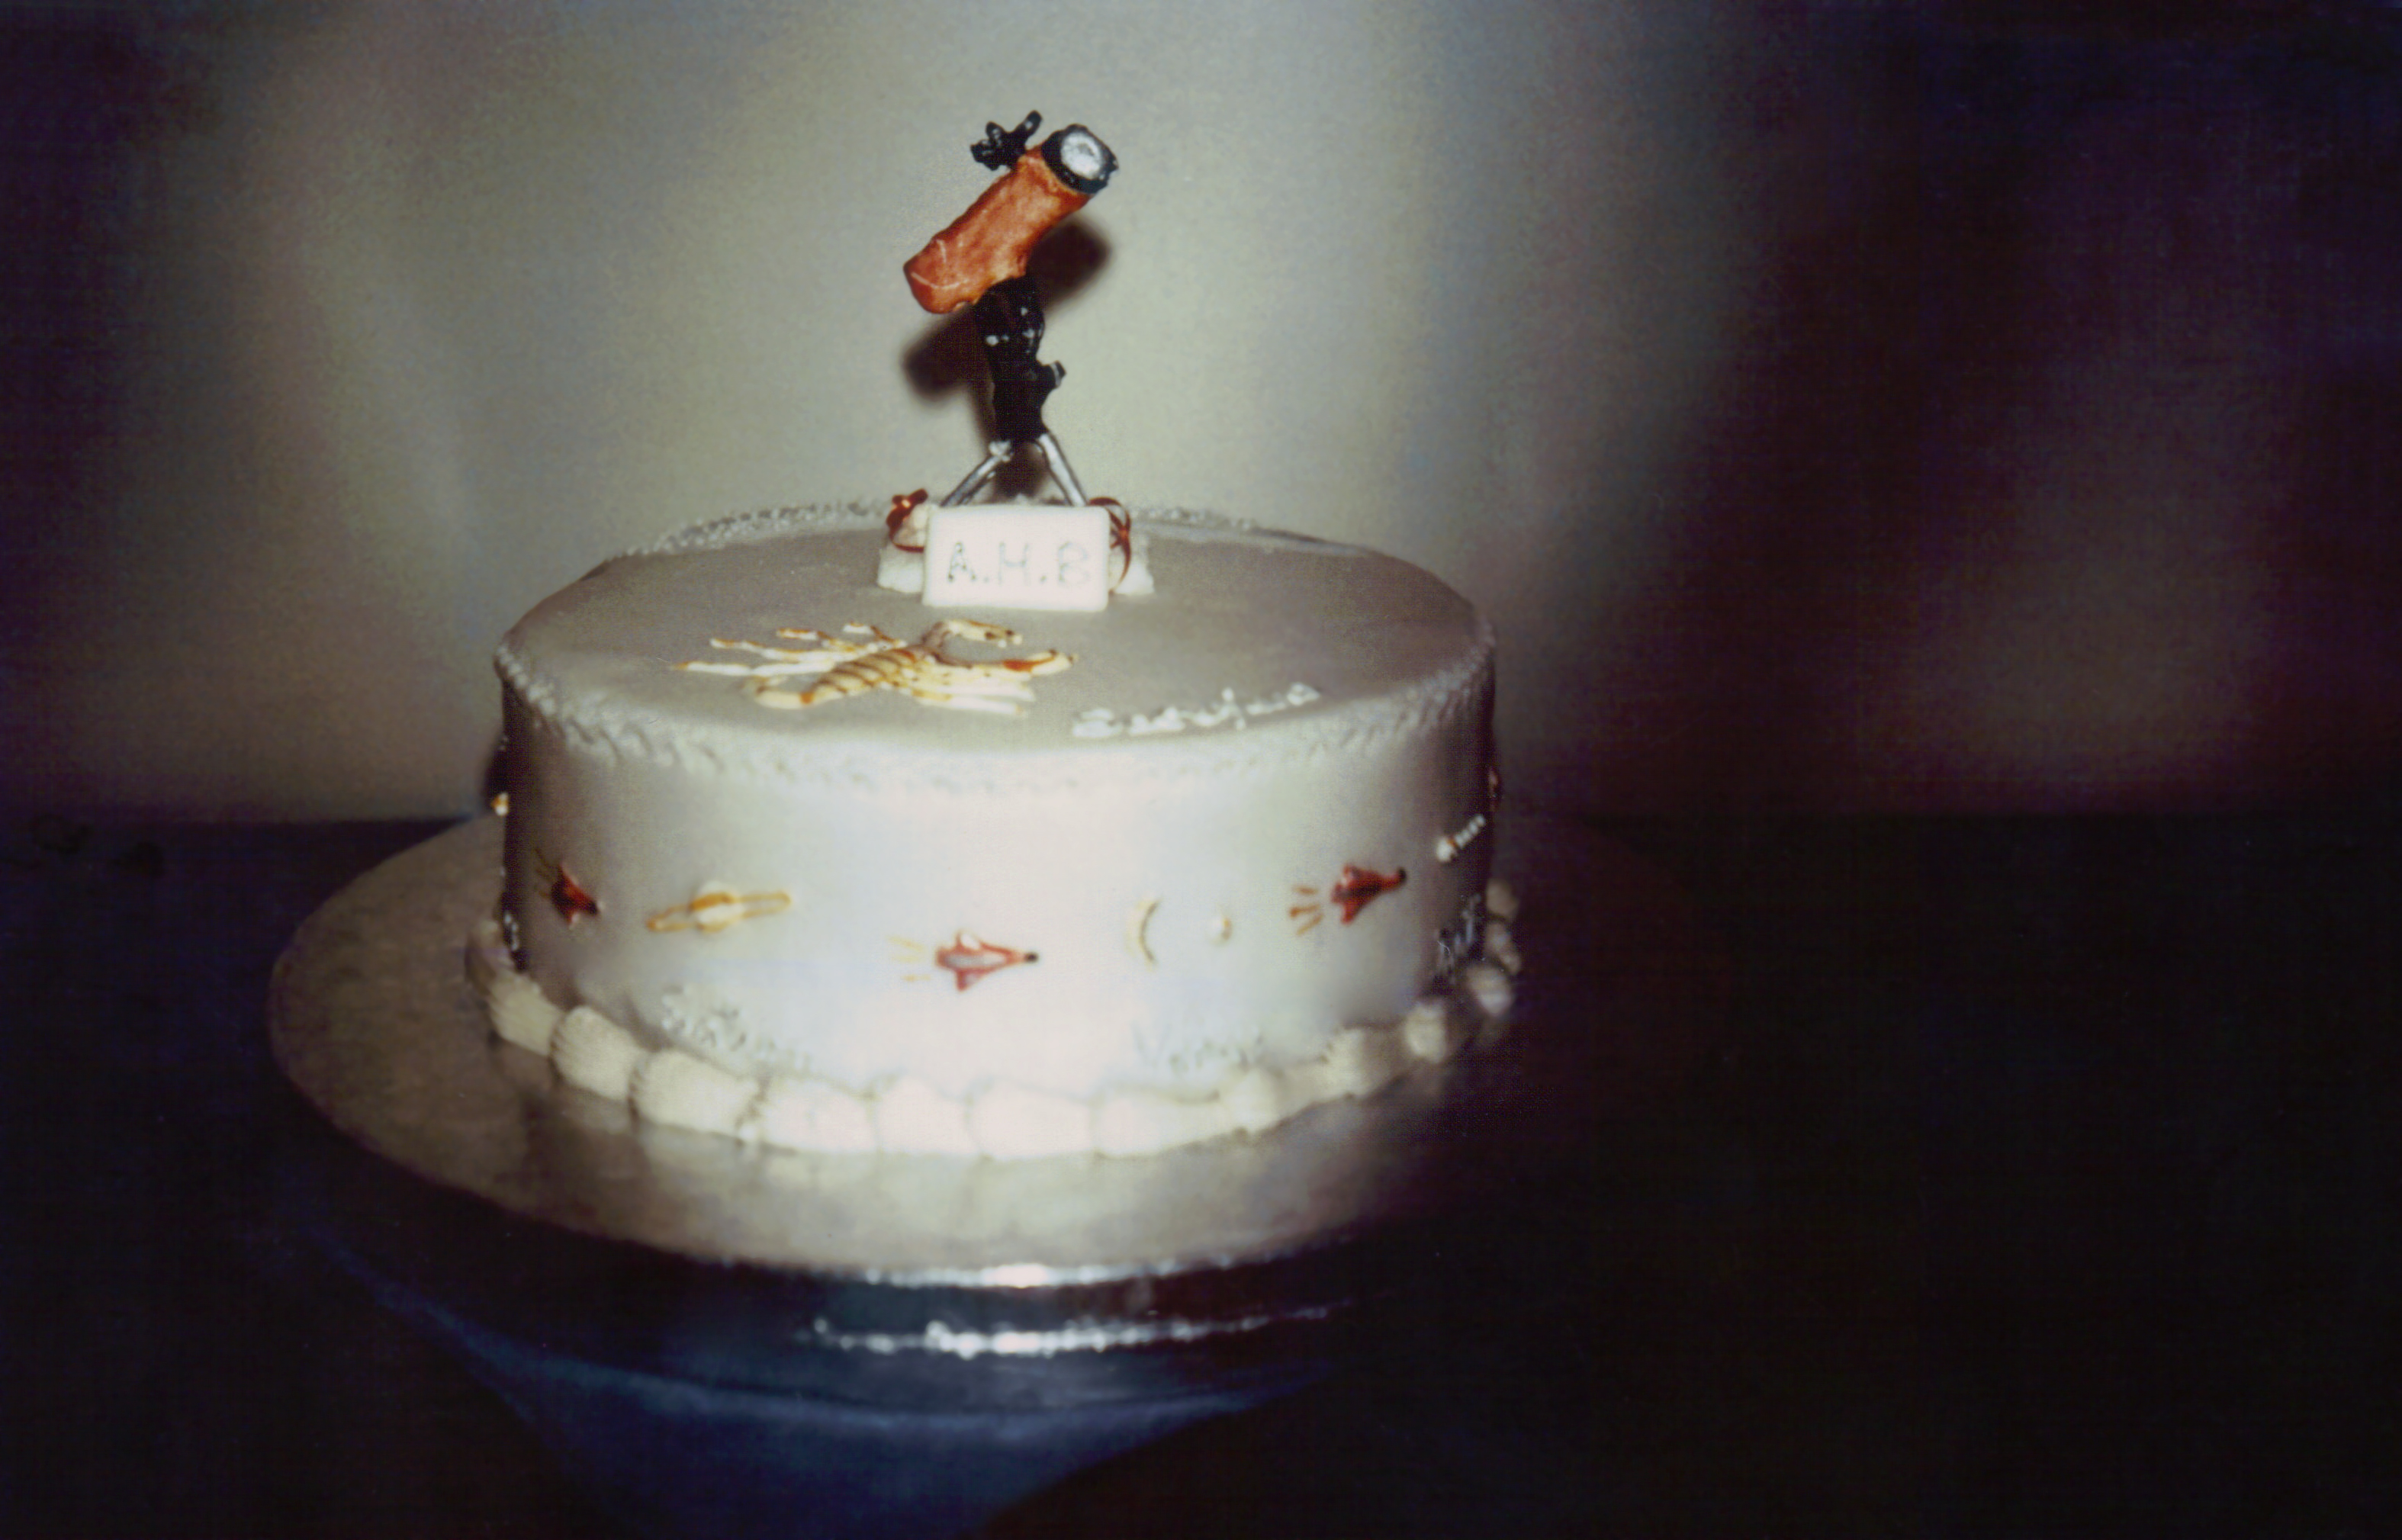
\includegraphics[width=\textwidth]{photos/cake-astronomy}
%   \caption{Tony's 60th birthday cake had an astronomy theme.}
%   \label{cake-astronomy}
% \end{figure}


We acquired another animal during our stay in Bryanston -- this time a
kitten Elizabeth had found and adopted whilst she was in residence at
the hospital. He was not allowed to stay there so we took him to live
with us. He was another handsome specimen and he grew into an enormous
cat - black with white ``socks'' and white ``bib''. He was called
Sydney (see Picture~\ref{sydney}). We feared for Sydney's life if he
came up against Sherman and tried to keep them apart but they met in
the gardens and took to each other. The cat was the tormentor and
would jump out at Sherman from behind a tree, but they were only
having some fun. Sydney did not like me and would leave a room if I
entered -- often leaving the comfort he found on Tony's lap -- his
favourite place. I often wondered how I had offended him!

% \begin{figure}
%   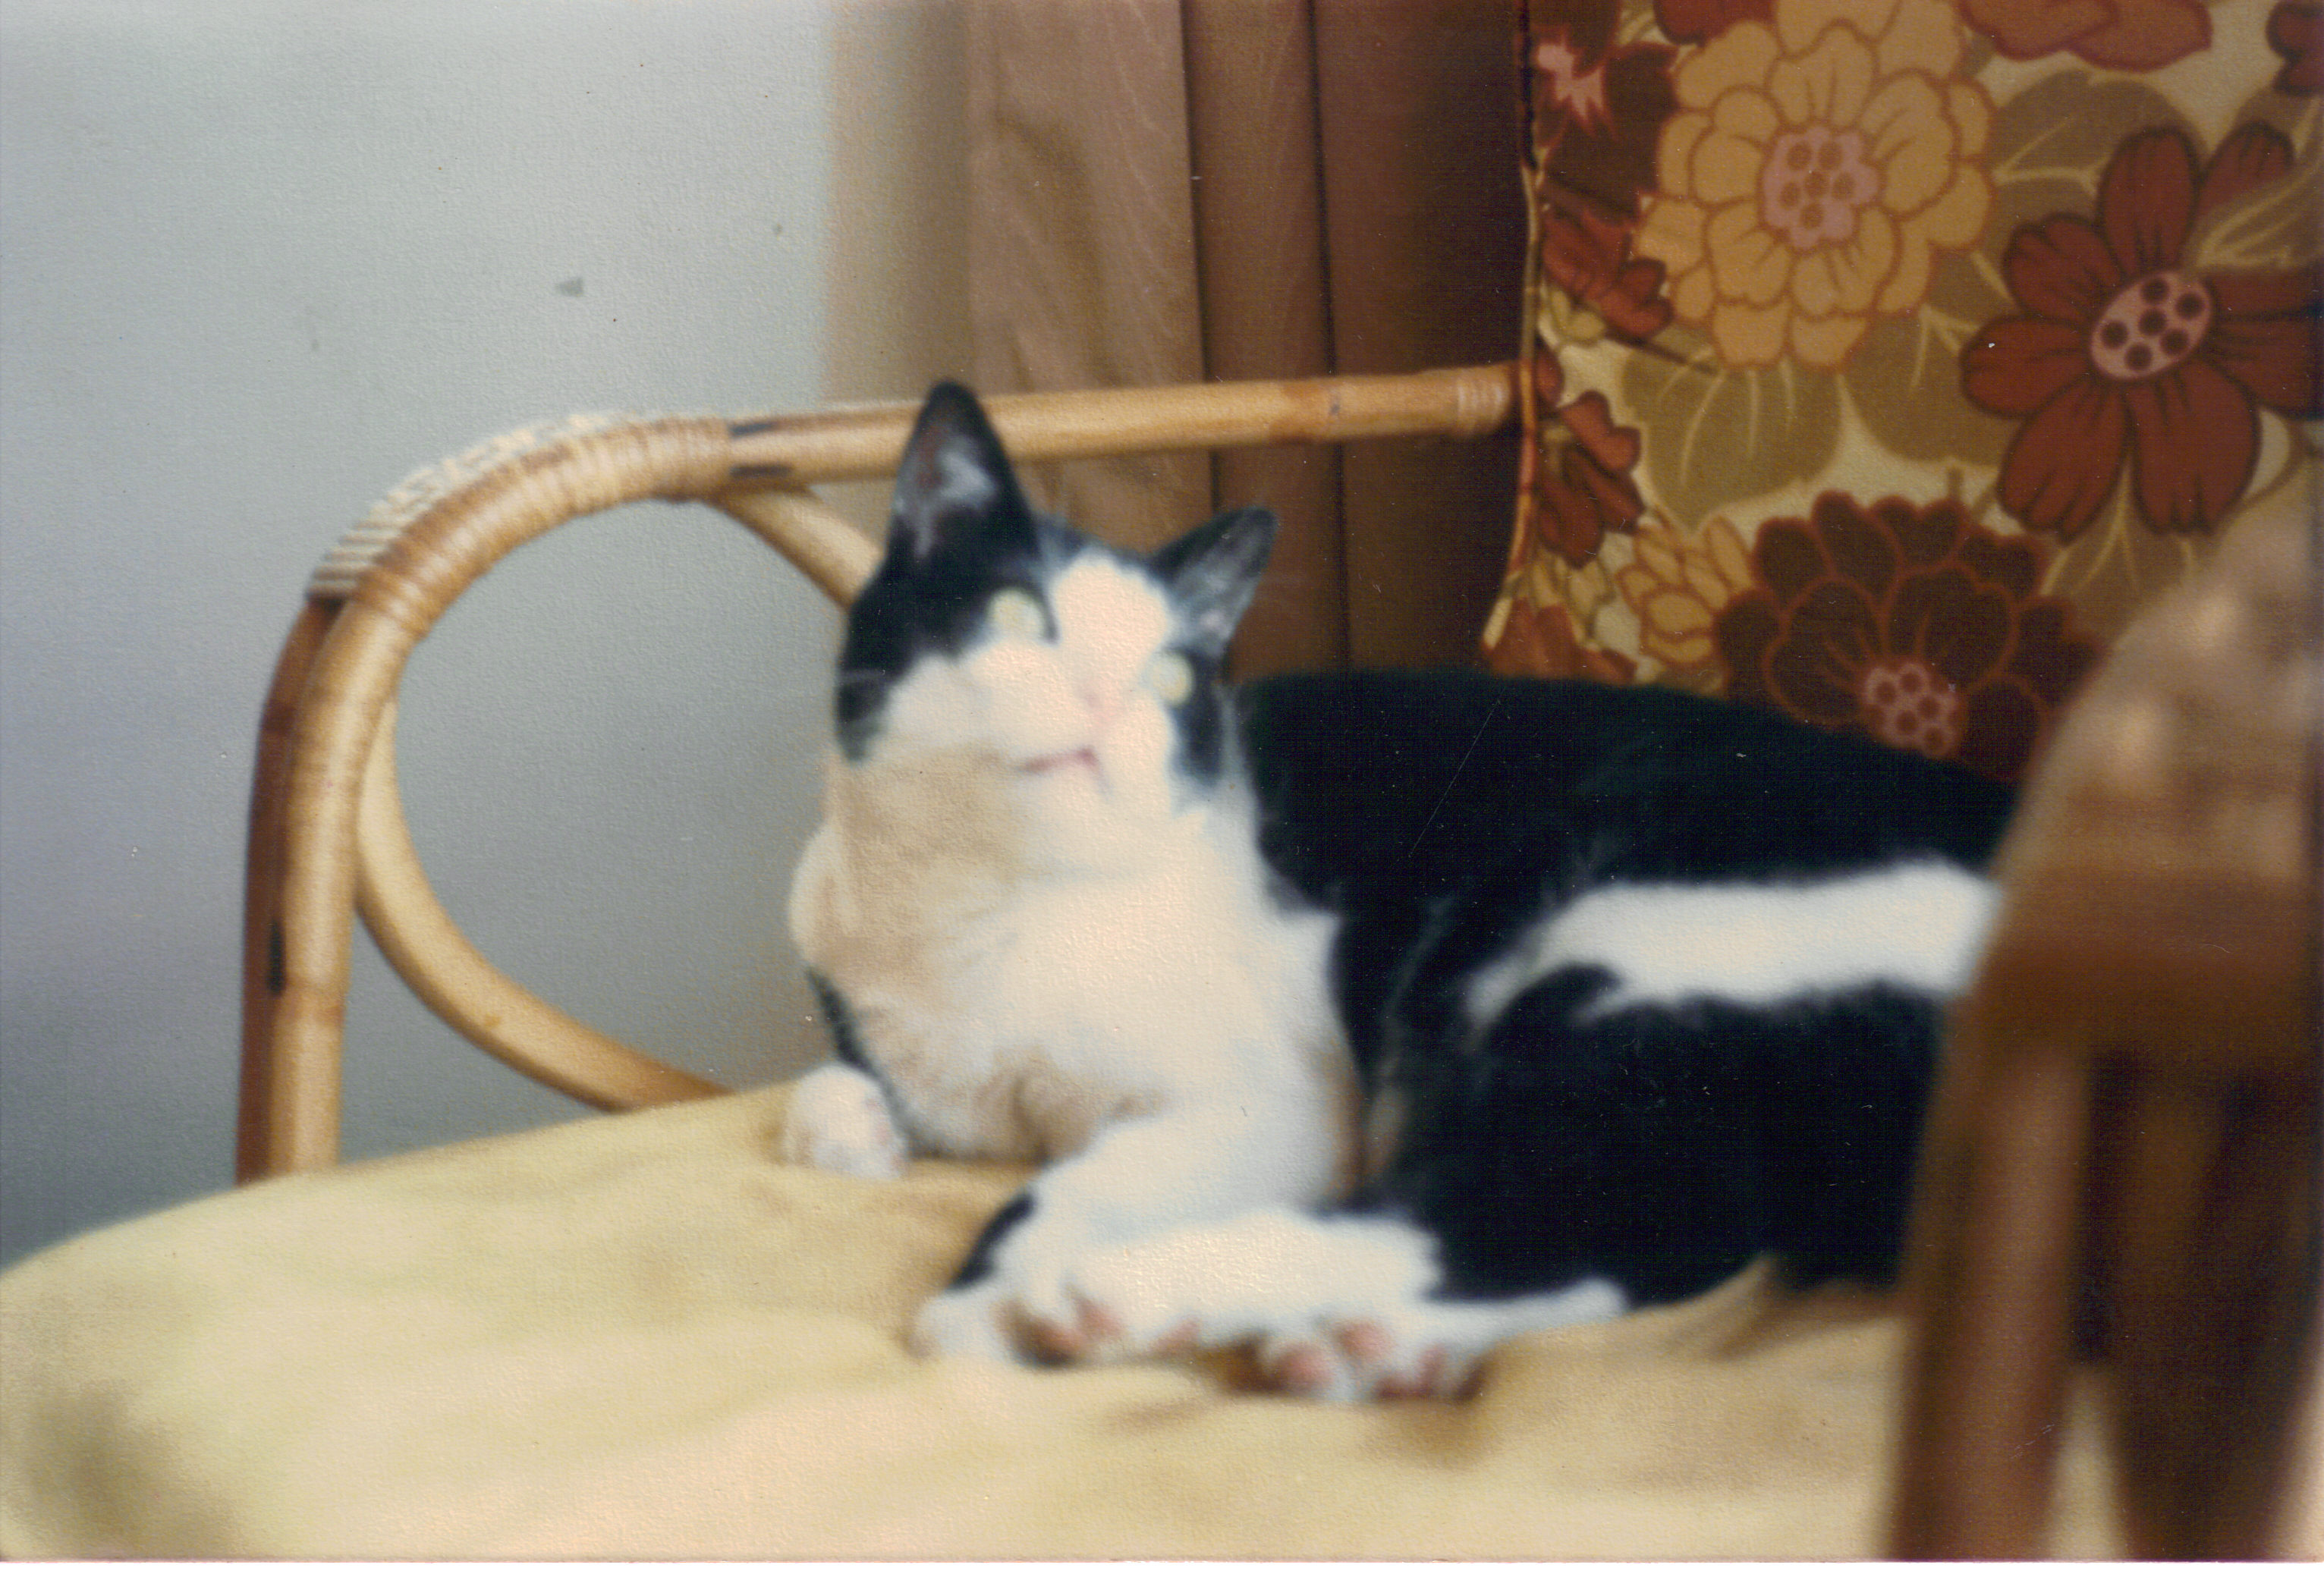
\includegraphics[width=\textwidth]{photos/sydney}
%   \caption{Sydney.}
%   \label{sydney}
% \end{figure}

Sadly both animals suffered illness and had to be put down; Sherman
was twelve and Sydney sixteen. We loved them so much that we cried
like babies and could not contemplate ever having another pet --
although somewhere along the way Elizabeth acquired a budgie.

Another joy about living in Bryanston was that Tony gave me a tennis
court (with lights) -- a most generous present. If people came in the
evenings we would play under the lights (no shadow). My tennis party
took place on Tuesday mornings: six to eight of us having a wonderful
time under a big tree with (naturally) refreshments and chatter (see
Pictures~\ref{tennis}). Looking back it was a superb time of life for
me.

\begin{figure}
  \centering
  \begin{tabular}{c}
    \subfloat{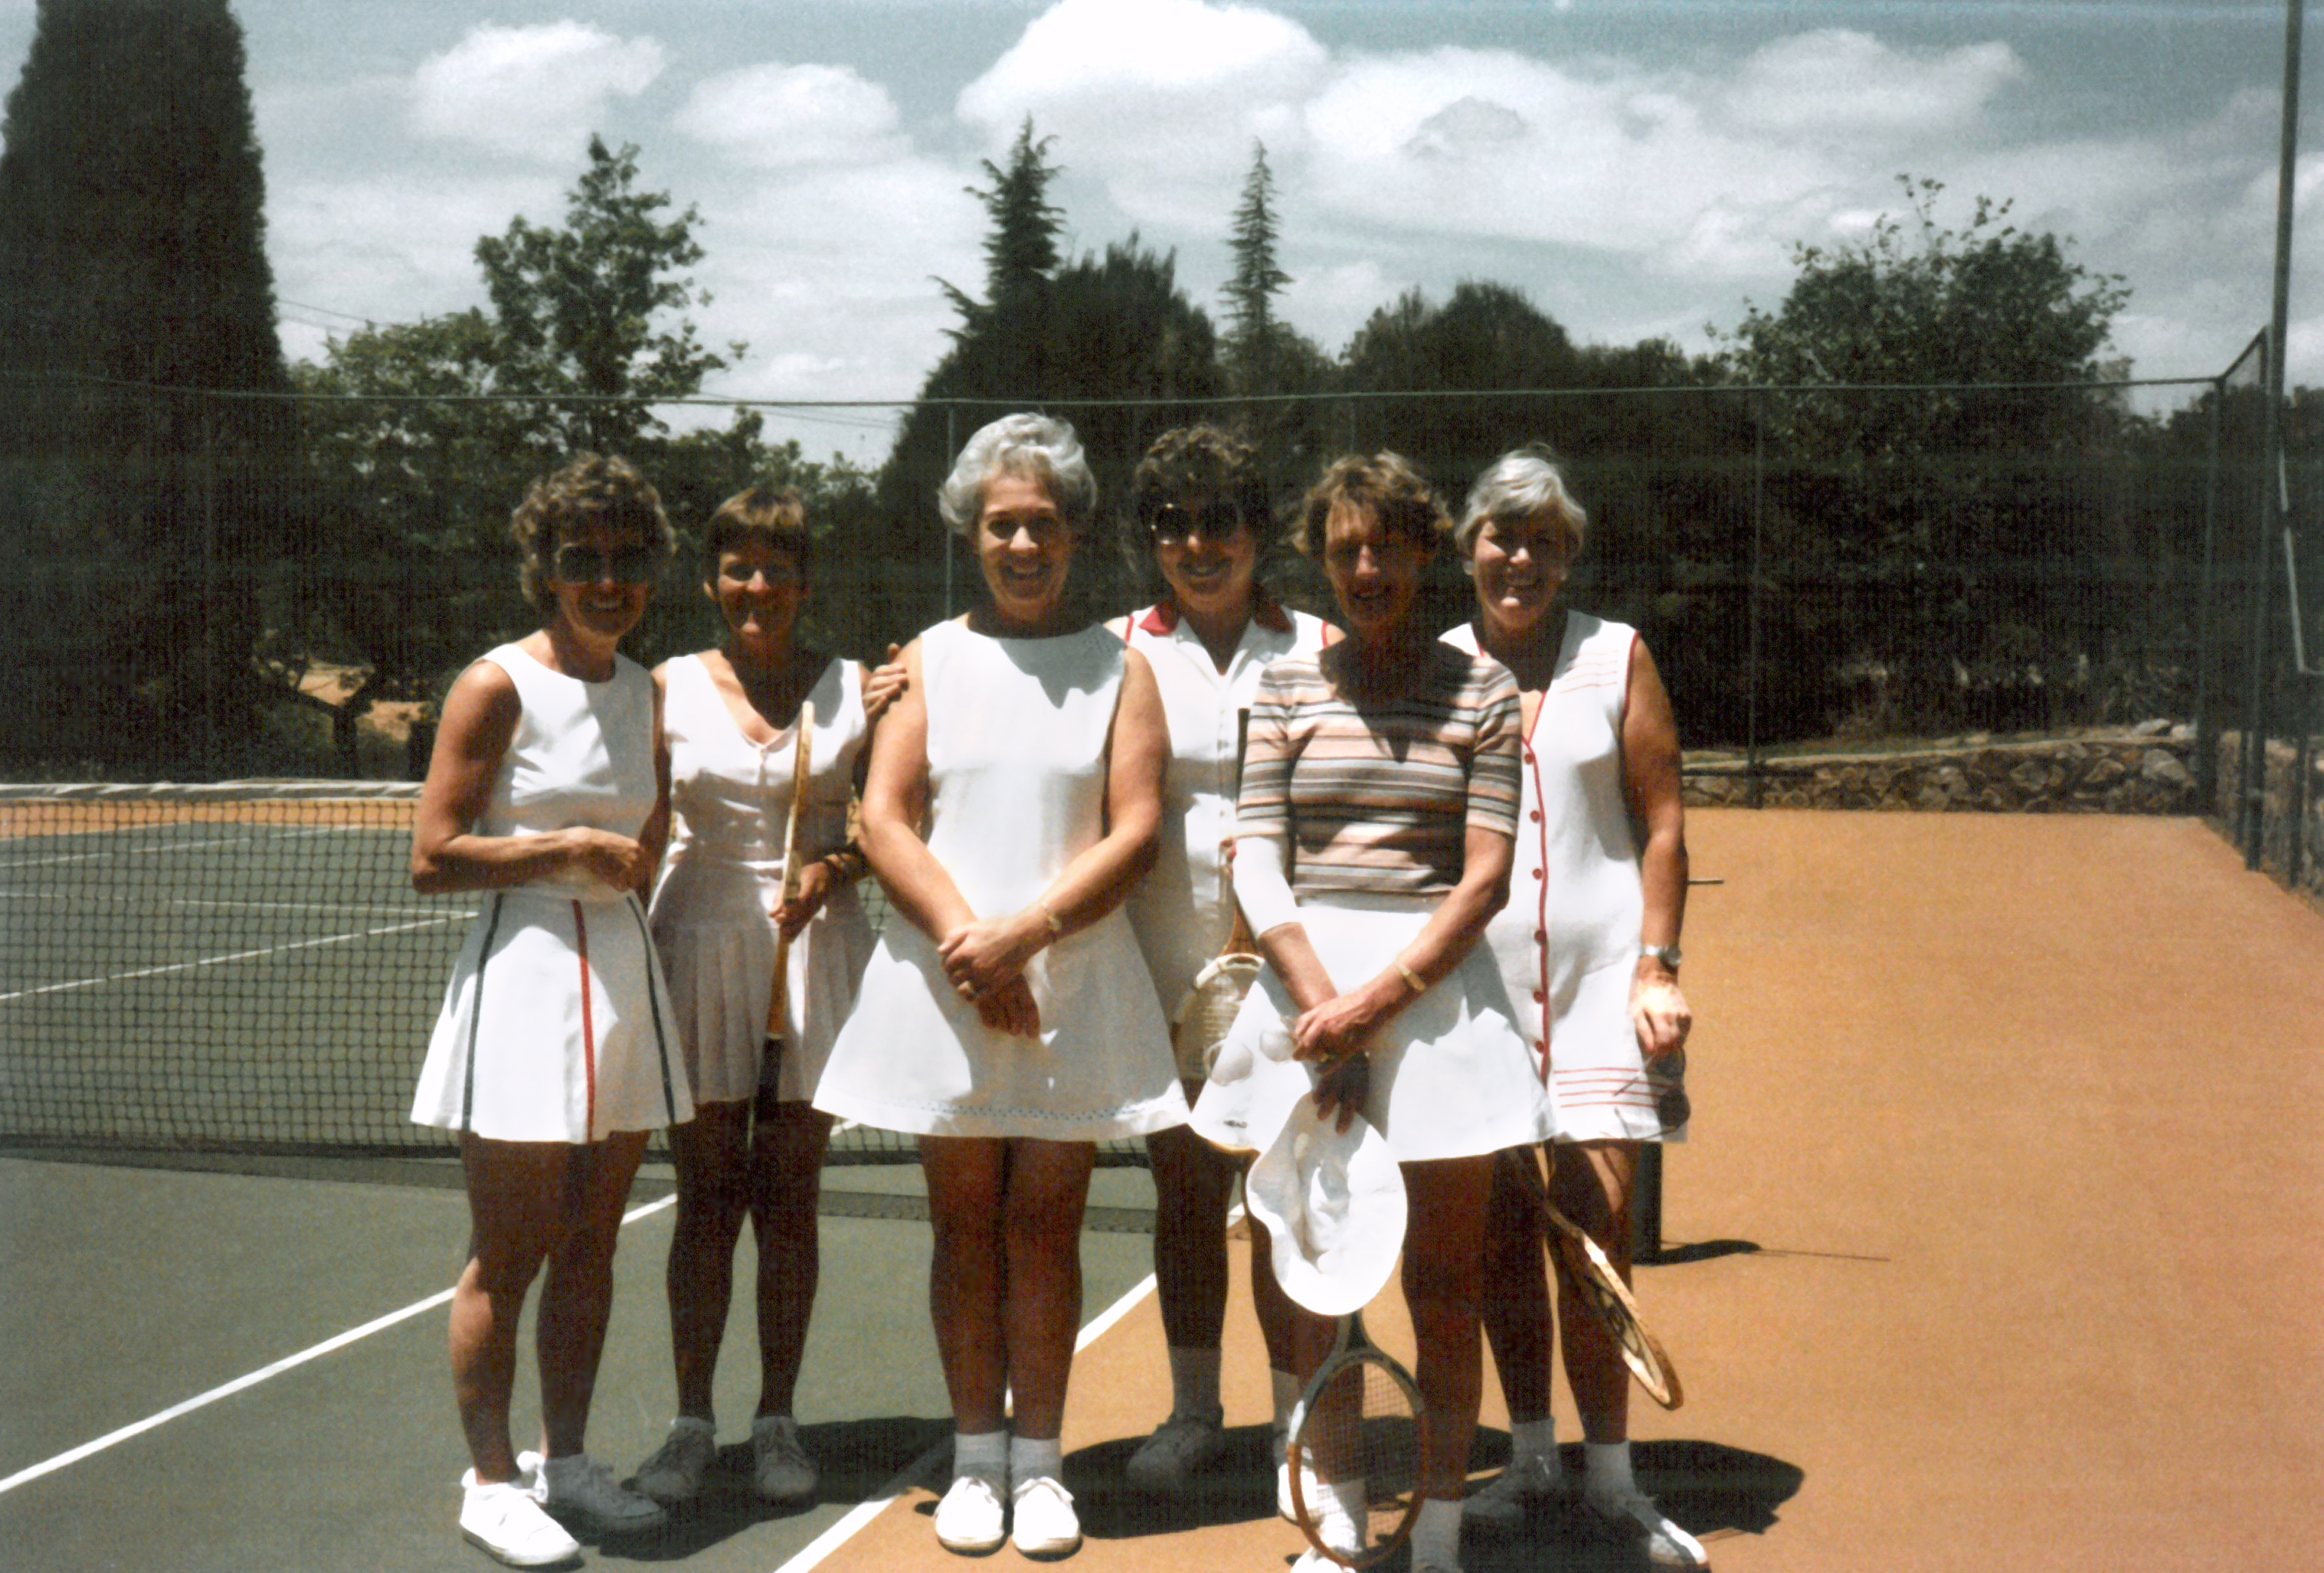
\includegraphics[width=0.9\textwidth]{photos/tennis-group.jpg}\label{tennis-group}}
    \\
    \subfloat{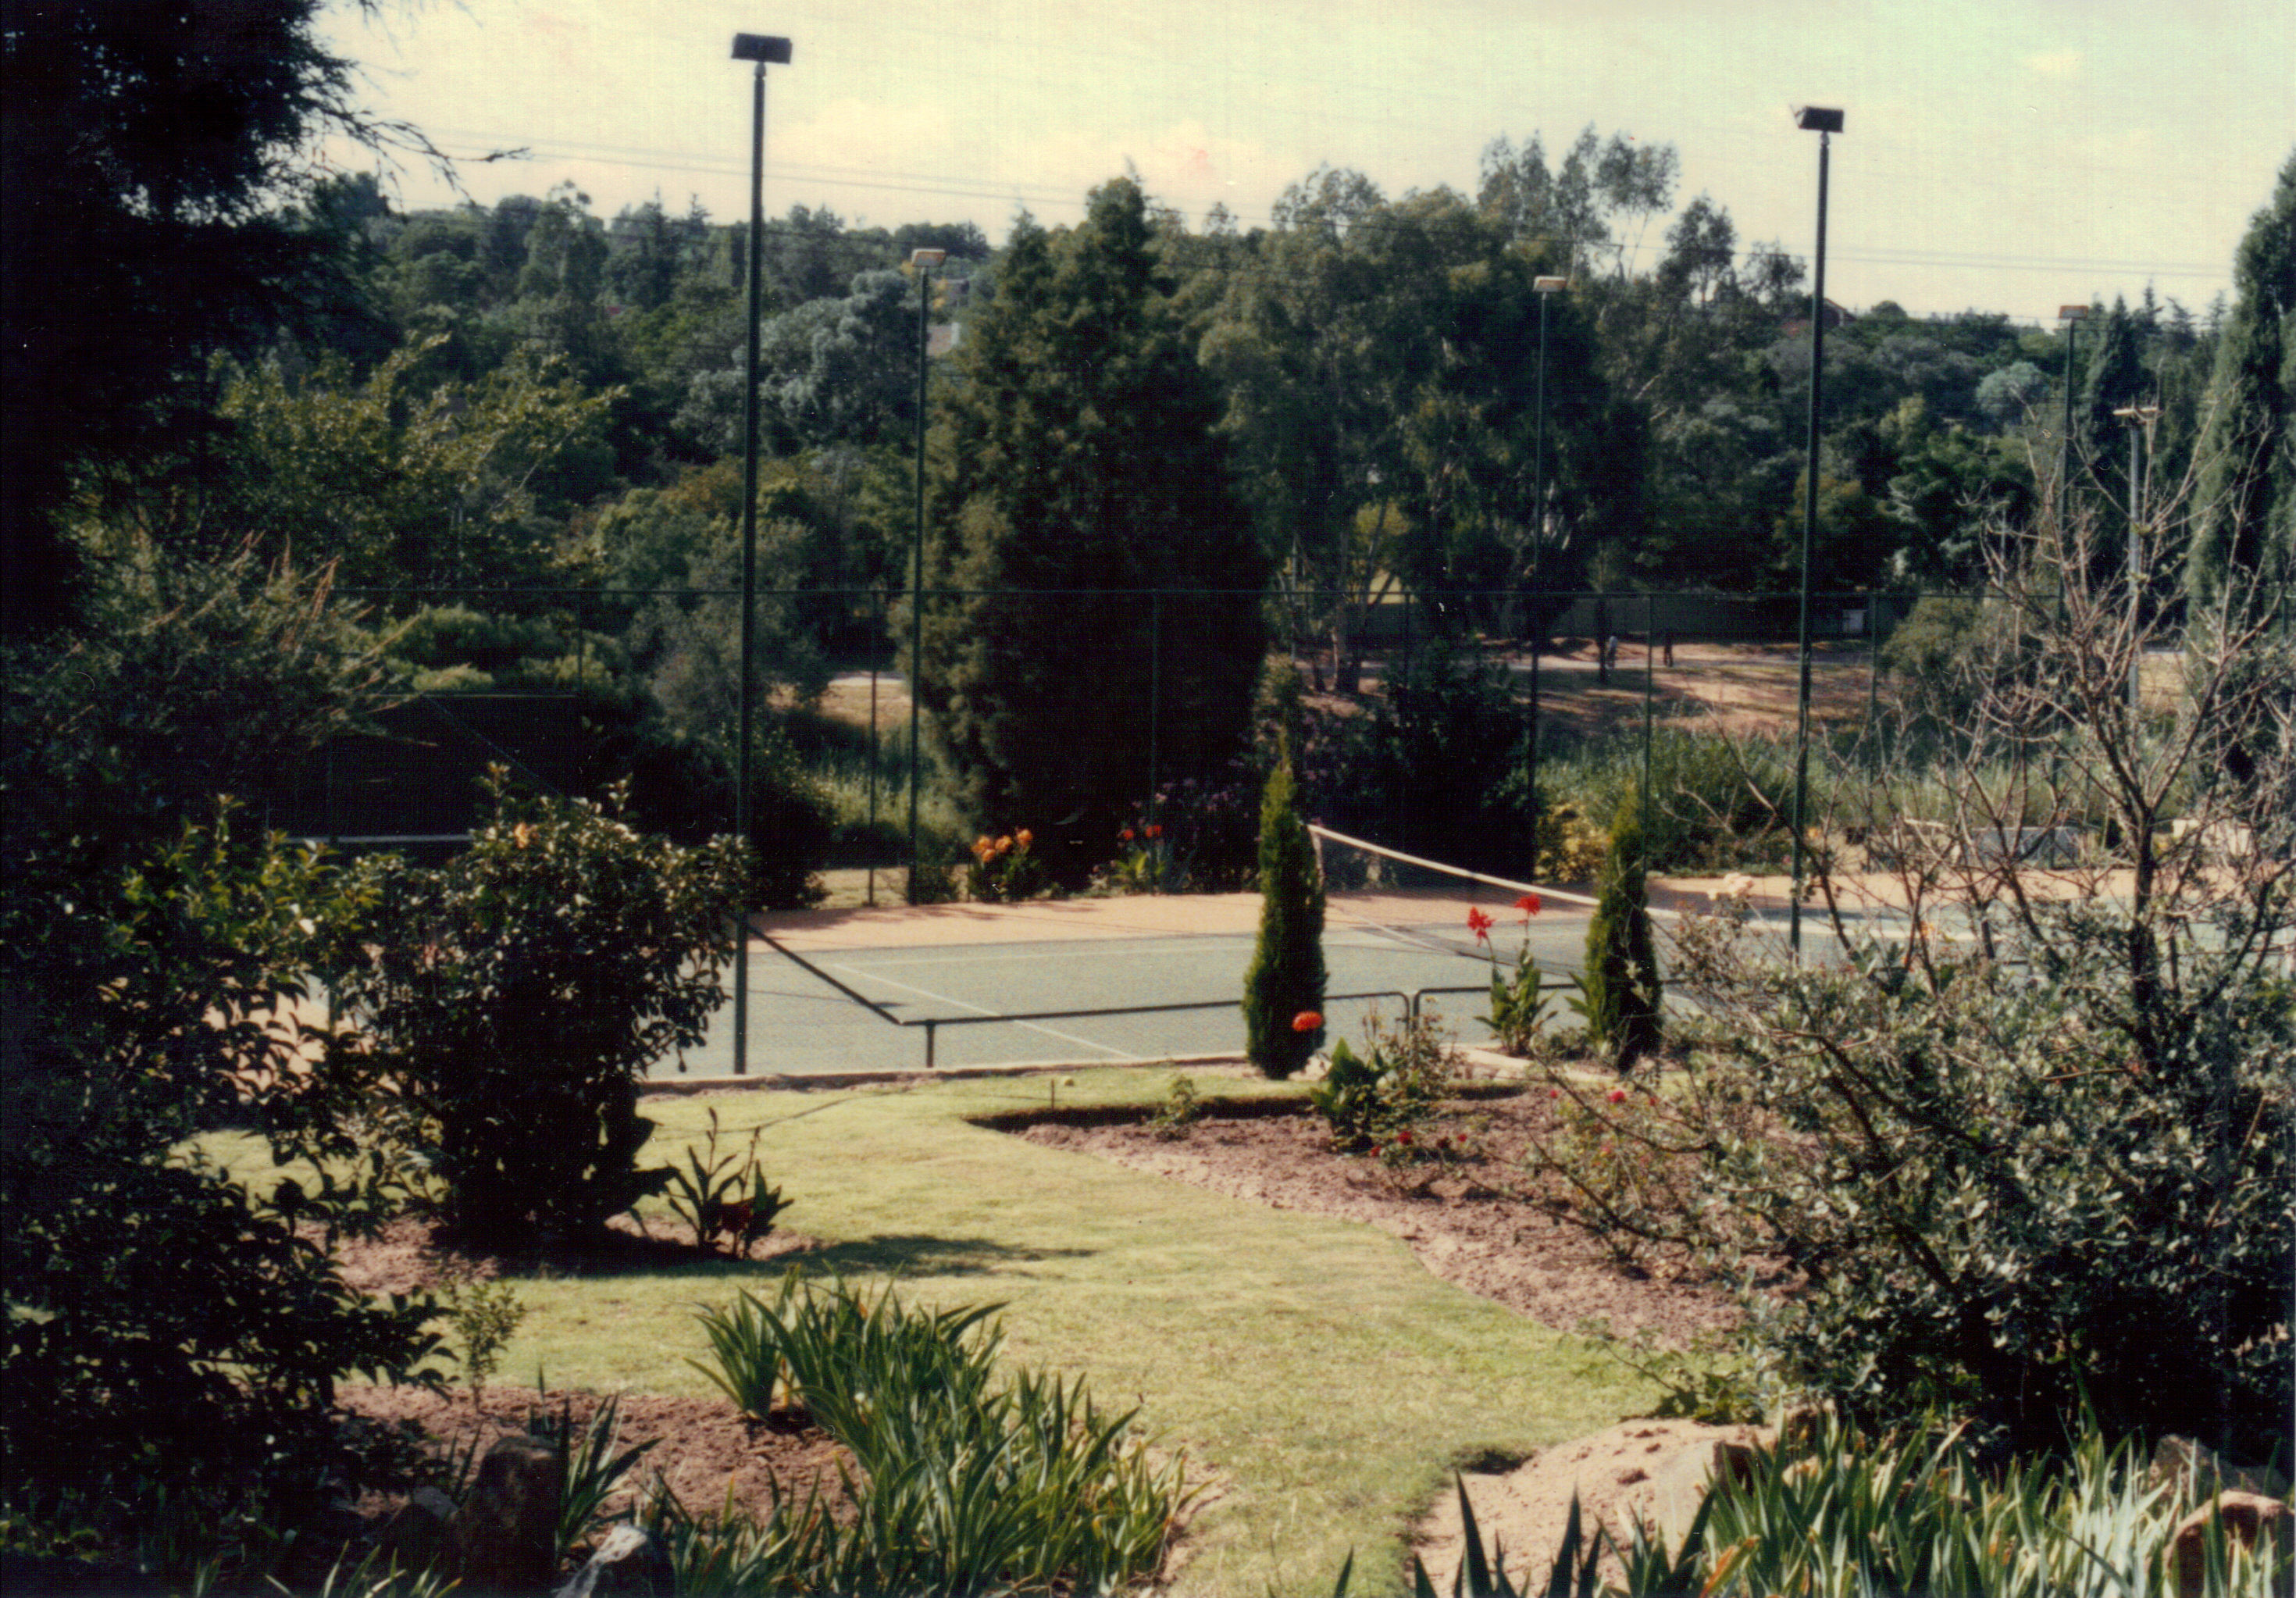
\includegraphics[width=0.9\textwidth]{photos/tennis-court.jpg}\label{tennis-court}}
    \\
  \end{tabular}
  \caption{Madge's tennis group and tennis court.}
  \label{tennis}
\end{figure}

% \begin{figure}
%   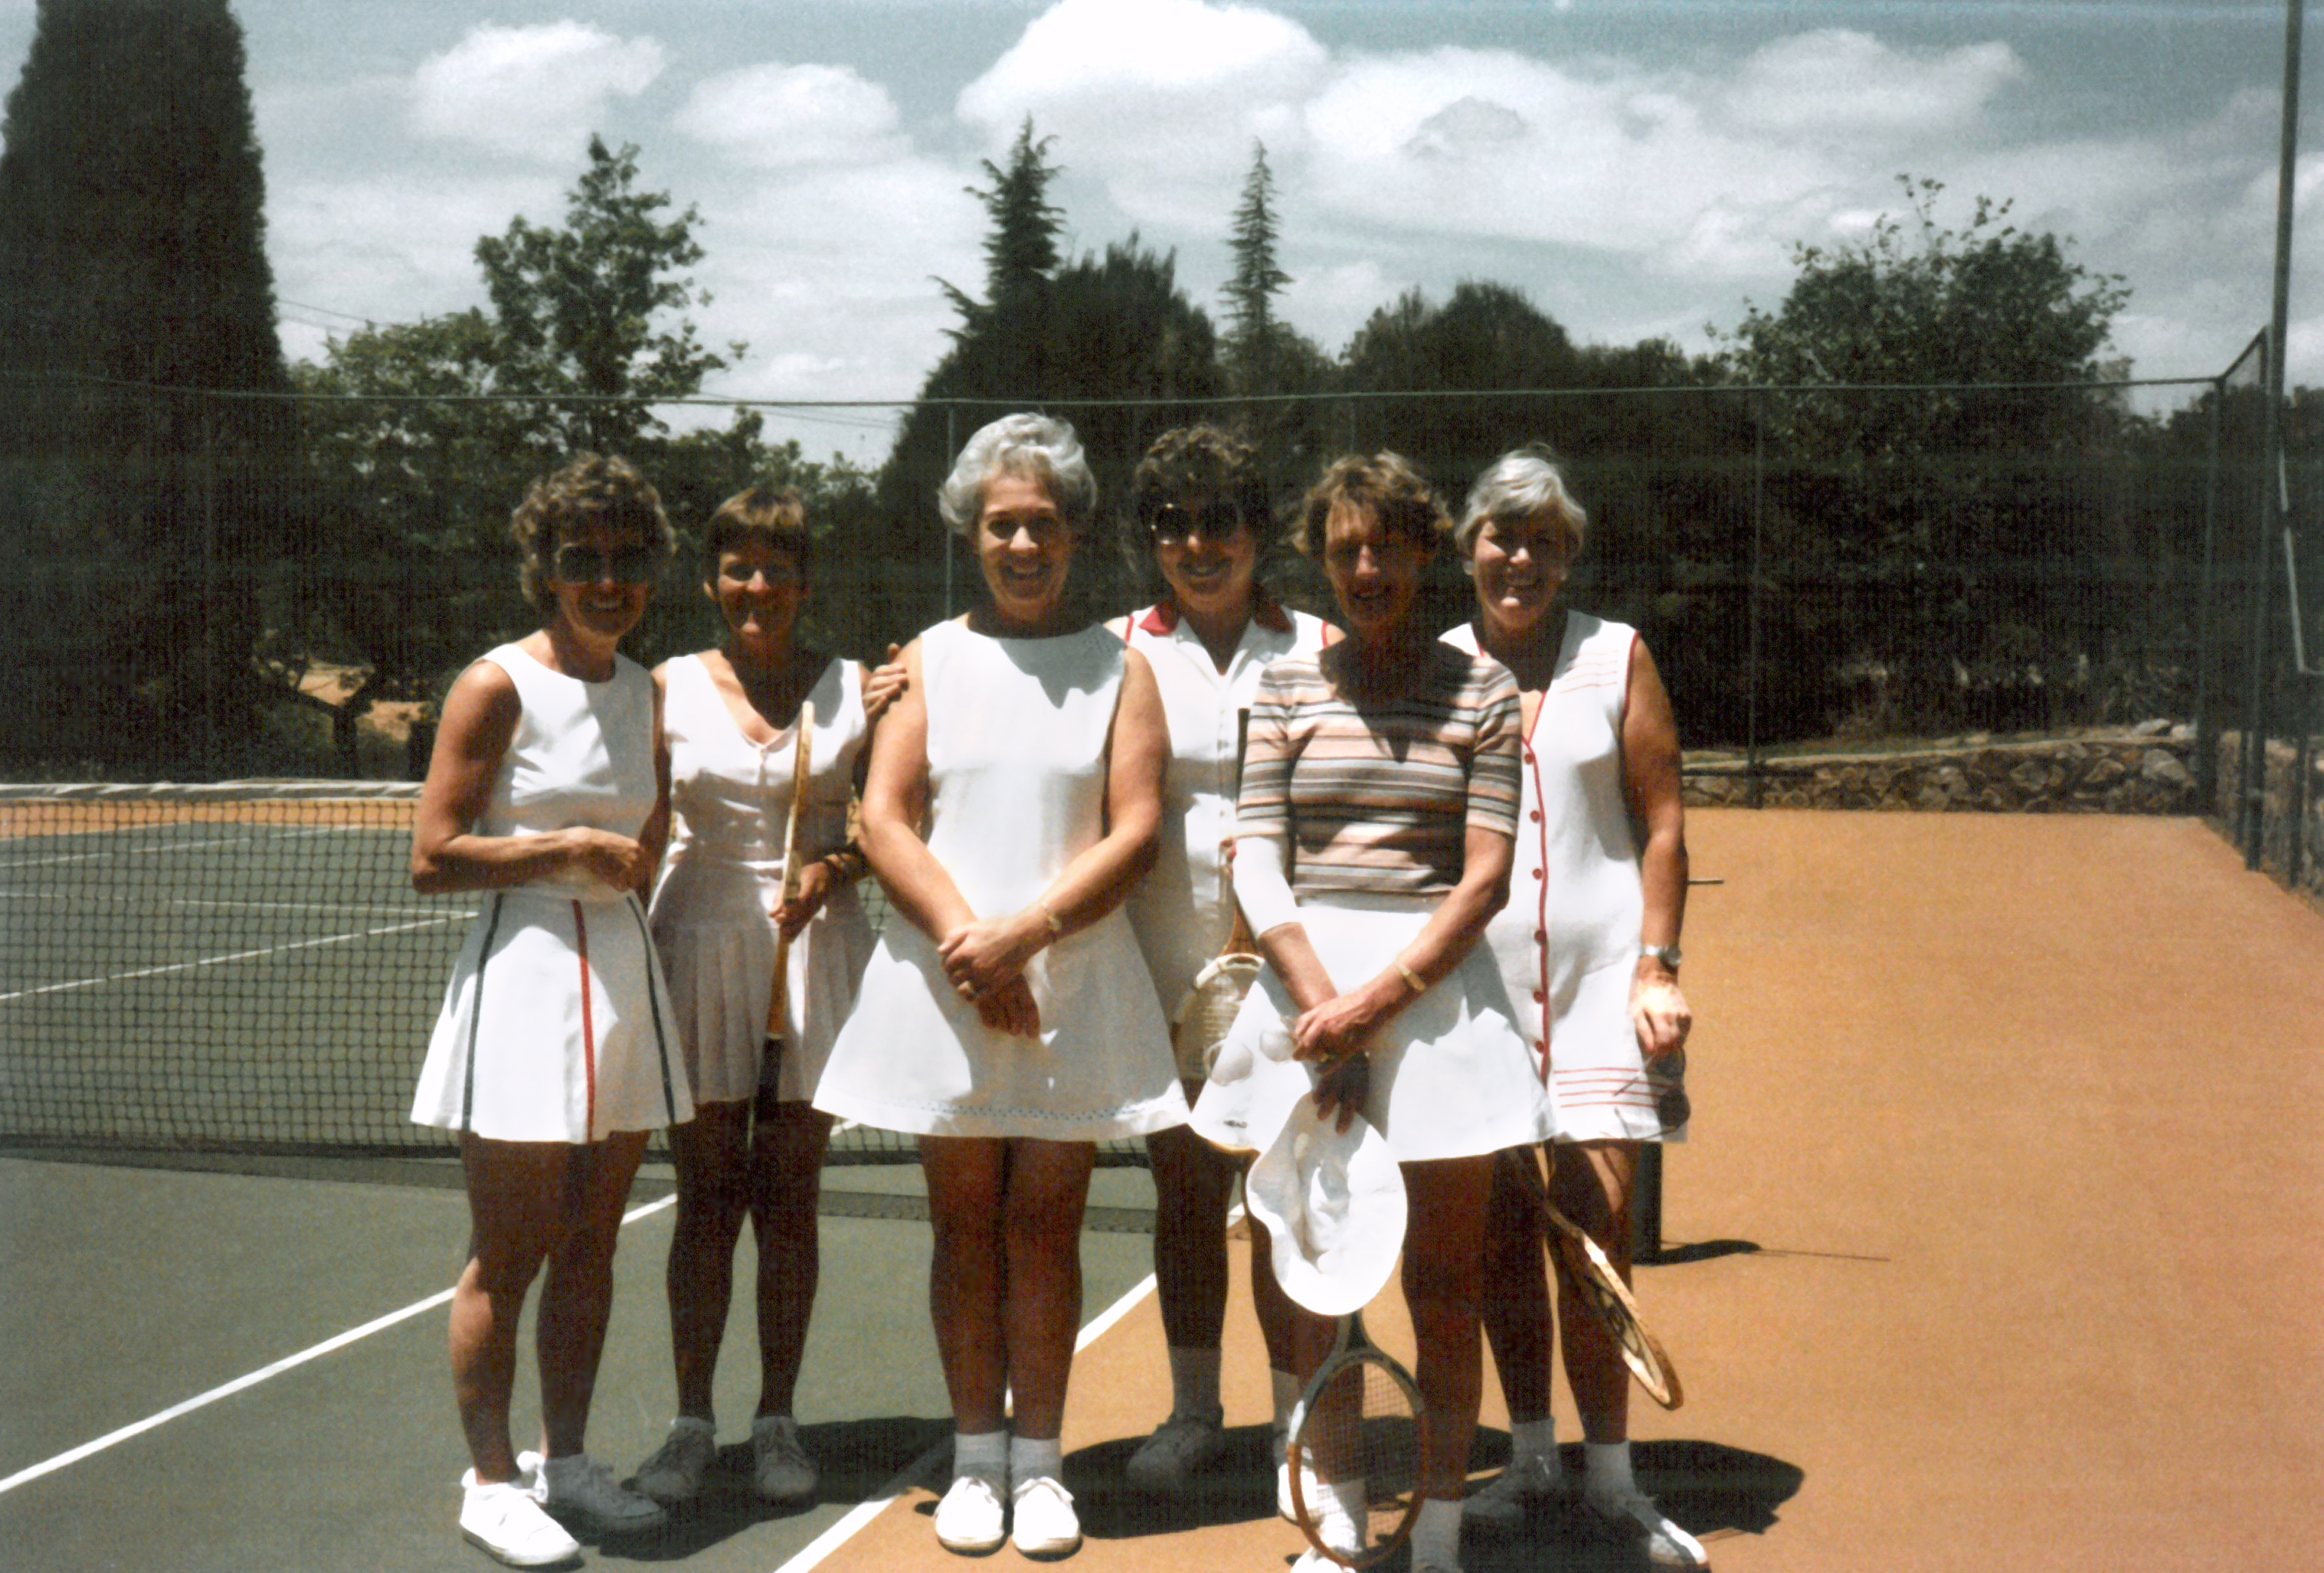
\includegraphics[width=\textwidth]{photos/tennis-group}
%   \caption{Madge with her tennis group (Johannesburg, 19??).}
%   \label{tennis}
% \end{figure}

% \begin{figure}
%   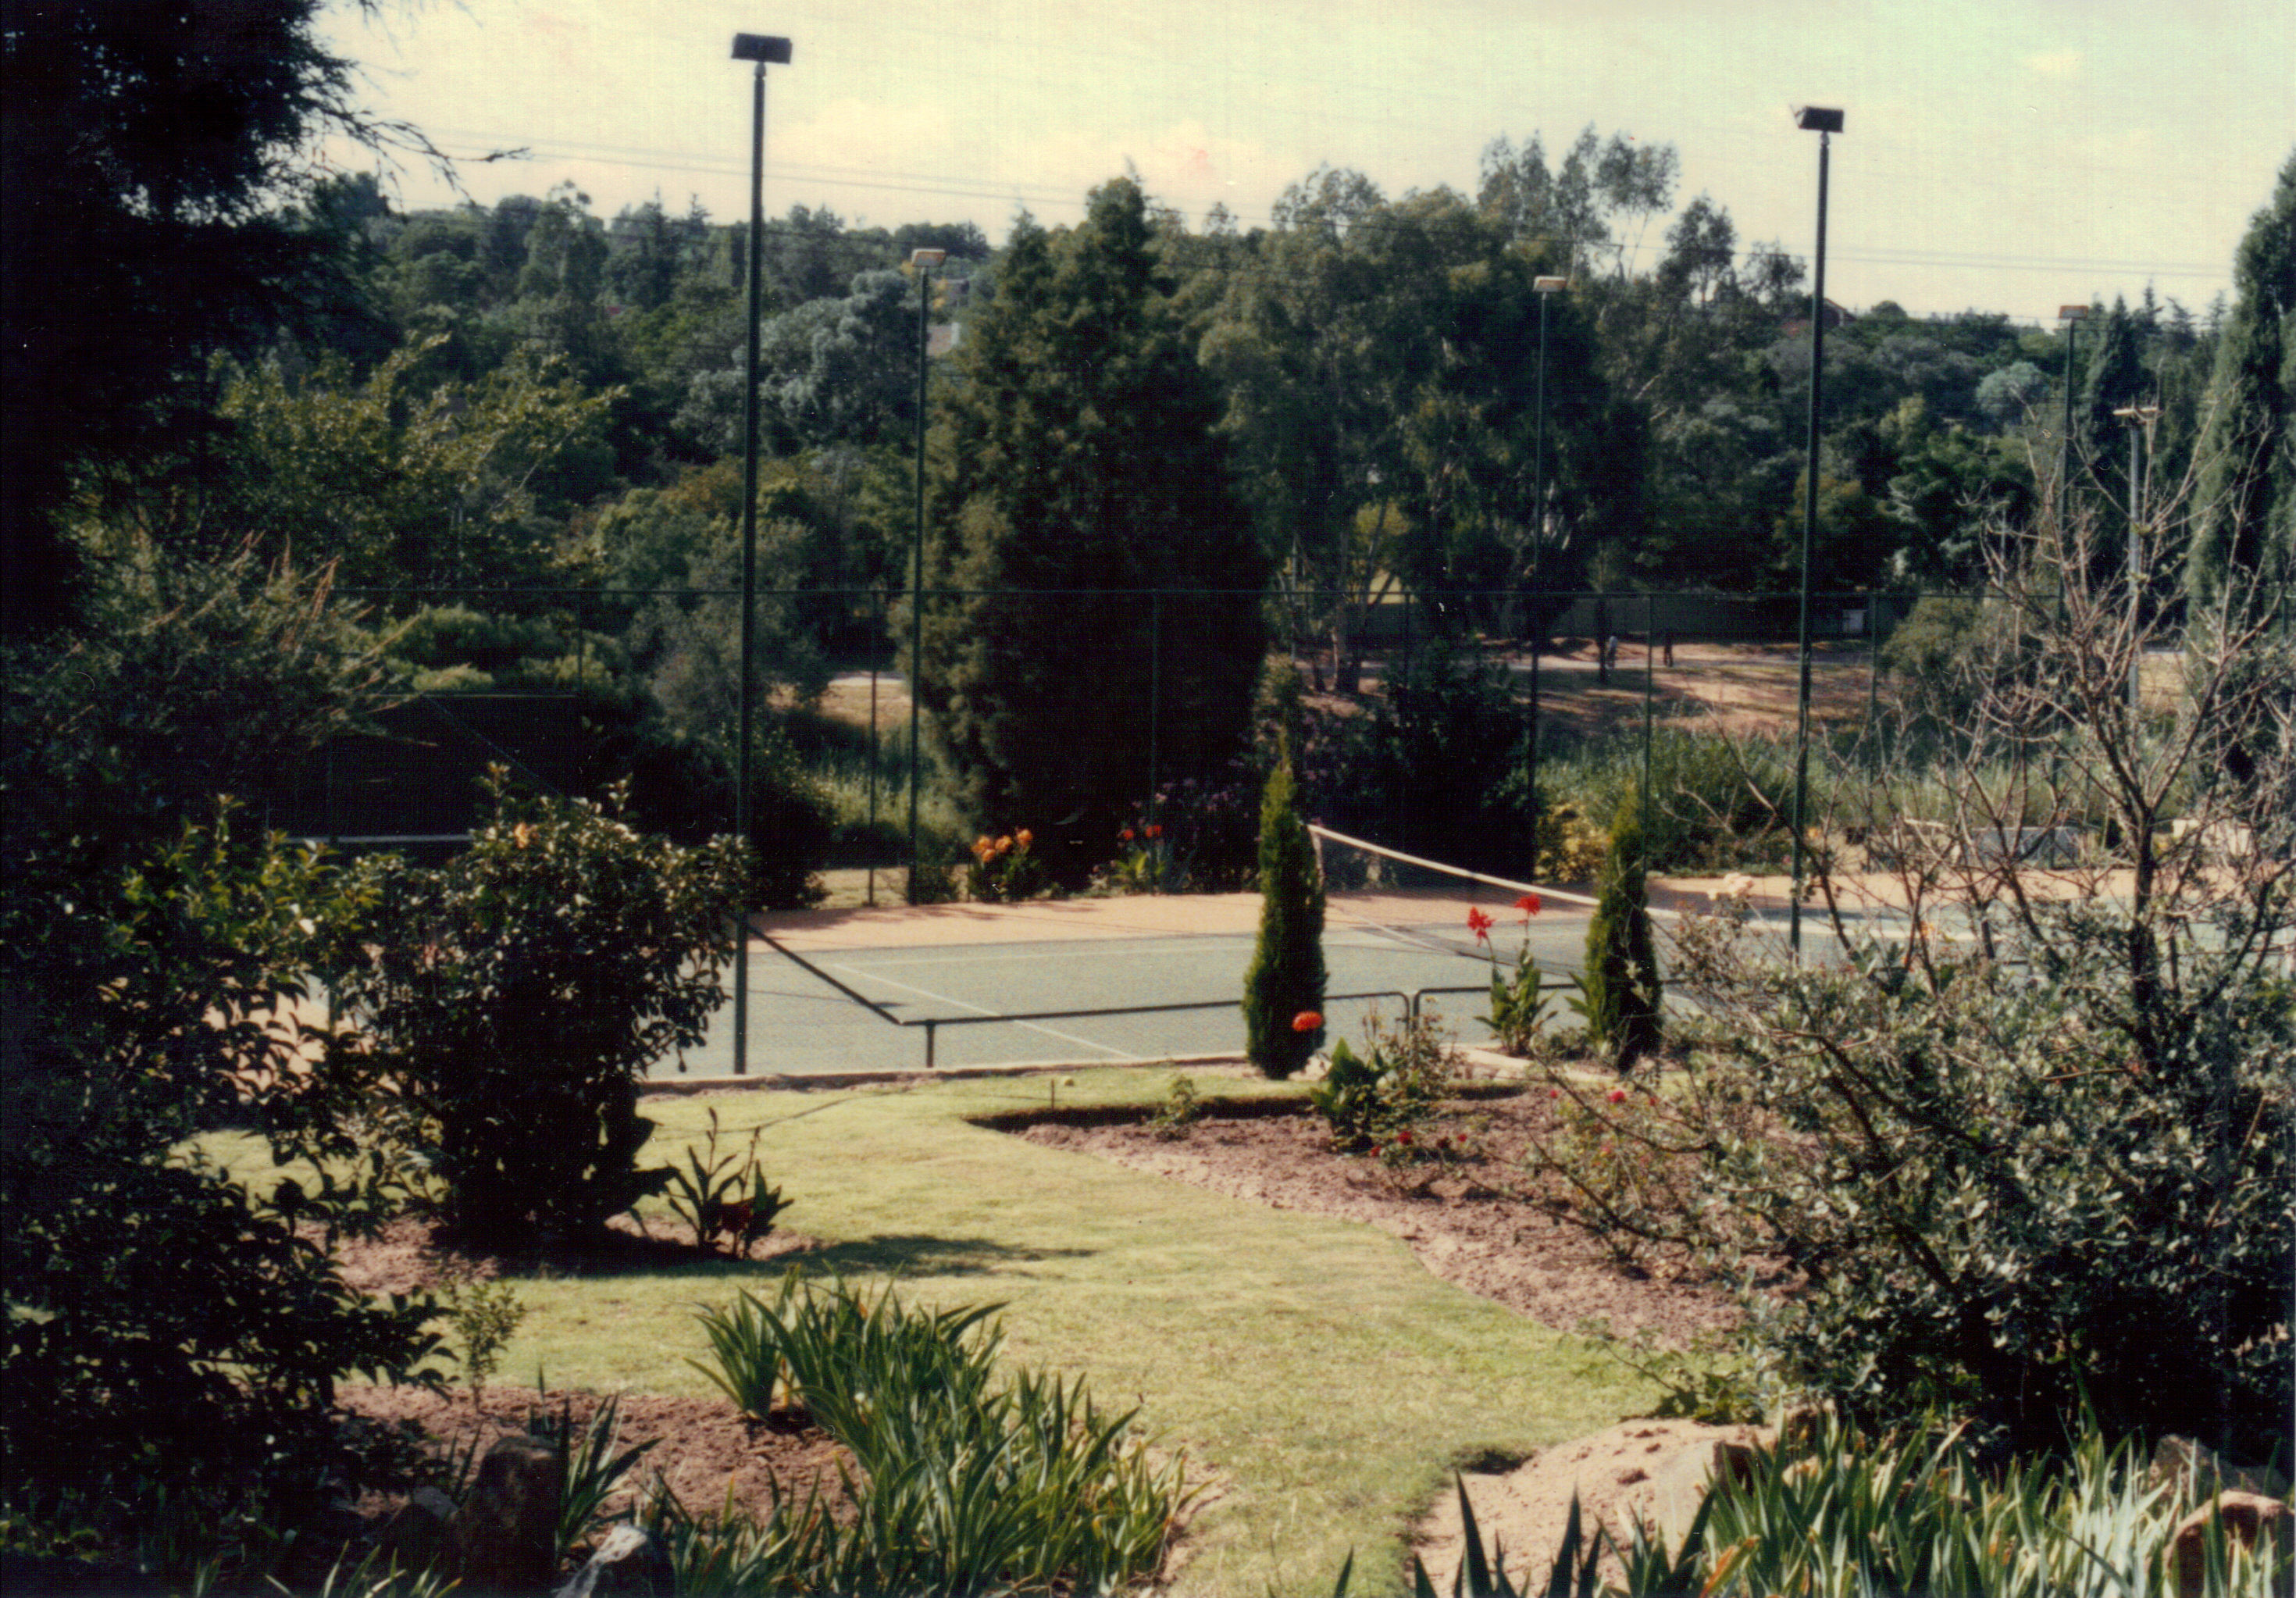
\includegraphics[width=\textwidth]{photos/tennis-court}
%   \caption{Madge's tennis court.}
%   \label{tennis-court}
% \end{figure}

At this time Elizabeth was at school at Roedean (we did not know then
that she was not happy there but she did very well anyway). Richard
went to St. John's college in Johannesburg and we had no idea that he
loved it! Being a weekly boarder, he had to be taken back to school on
Sunday evenings and got extremely upset about being left but,
apparently, pulled himself together very quickly. Little devil!

Sherman had a lovely nature -- but \textit{could} be nasty if
necessary and he became a wonderful friend and companion to us all --
particularly to me as I spent much of the day alone. He joined us when
he was two and lived to fourteen. Sadly arthritis and a growth on the
liver caught up with him and he had to be put down.

A cat also came into our lives and he and Sherman became good friends.
The cat (kitten then) was really Elizabeth's but it became impossible
(and not allowed) for her to keep him in the hospital where she was
training in nursing (and achieved her B.Sc.) So we took him on and
loved him. He adored Tony but did not like me. If I entered a room he
would even jump off Tony's lap and leave the room -- even though I was
the one to give him his meals and try to stroke him. Sadly in his old
age he became ill -- and very fat and incontinent -- and we had to say
``goodbye'' to him too.

We never wanted another animal to replace these two who were
outstanding.


\chapter{Israel}

Whilst working for the GEC in Nigeria, Tony had business dealings with
an Israeli company and, on one of his visits to Israel, he took me
along. Being in the Middle East, there were strong resemblances to
Turkey and I felt really at home.\footnote{This was a 12~day trip in
  1984. Elizabeth was married and had just had Andrew. Richard was 20
  and embarked on his hotel training.}

Tony hired a guide for us whose name was Teddy Vardi and we were so
lucky to be looked after by him. He seemed to know every inch of the
country and Israel came alive to me. It was magic to me to go to
places where Christ had walked; I was swept away by Jerusalem.
Learning what had happened there and the history etc. was
mind-blowing.

In Teddy's car we covered so much of the country and he described
everything so well. We saw many places: Tel Aviv, Tiberias, Hebron,
and etc. I had to write down all we had seen every evening; it would
have been impossible to remember it all.\footnote{I wrote a journal
  which accompanies these notes -- see Appendix~\ref{Israel}.} I
remember so well going to Masada, passing by Jericho and the Dead
Sea. Masada is the place where so many Jews were massacred under
Herod's instructions. There must have been survivors for the story has
been told.

Another story, of course, is the massacre of the 6 million Jews by the
Germans before the outbreak of the second world war. It was
heartbreaking to visit the Yad Vashem, which is a monument to the Jews
who perished in the holocaust. A flame is kept permanently burning in
memory of those who perished. My memories are so clear about his
country and certain occasions do stand out -- the Friday evening
dinner with Gurion and Sara Meltzer (in Tel Aviv) when we were the
only gentiles. It was such an honour to be there.

It is altogether different to read about a place and then to visit it
and try to absorb the religious and historical aspects of it. My walk
up the Via Dolorosa where Jesus had carried his cross to the place
where he was to be crucified was unforgettable.

Goodbye to Israel. What a host of memories.


\chapter{Retirement}

Tony enjoyed his managing directorship but arrived at the moment when
he decided, at age 63, that he would like to take early retirement.

He had been quietly studying his beloved physics and astronomy as he
had done for many years and decided that now was the time to buy a
telescope. This was done through the Johannesburg planetarium and with
the help of Tom Geary and Wim Ahlers we found such joy and pleasure
from that wonderful instrument and Tony taught me so much about the
``heavenly bodies''. Really mind-boggling bits of information like --
``planet Earth could fit into planet Jupiter 1,000 times'' will always
stay with me.

After fourteen years in Johannesburg, we decided to move to Durban --
not only because Elizabeth and Matthew lived there, but also because
Natal offered a quieter and slower way of life. And so we found a
beautiful house (much too big for a retired couple, but we loved it)
in Winston Park, Gillitts. We had a super life there with much
entertaining. And, of course, the beloved telescope occupied much of
Tony's time and he started to enjoy inviting school children to come
and observe the skies. Our neighbour was a teacher and her garden was
used for ``viewings'', being less full of trees to block the
views. Oh! How those children loved those evenings, and the teachers
and parents who also turned up were fascinated by listening to Tony
pointing out stars and planets etc.; what a wealth of knowledge he had
and how he was appreciated.

When the Preston family left South Africa to emigrate to New Zealand
we were devastated and missed them terribly. But the time and
opportunities came for us to visit them and altogether we made four
trips, using a different airline each time. We were able to enjoy the
sights and delights of the different places we stopped at -- Hong
Kong, San Francisco, Sydney, Singapore, etc. I remember well the
cleanliness of Singapore and the beauty of the gardens with their
profusion of orchids -- and even the airport (once the Changi prison)
was decorated with orchids from end to end. In Singapore, also, we
went across to Sentosa Island to the museum where there are horrible
images of the Japanese occupation but also the triumph of the
Singapore people to regain their country and to make it so lovely
again.

In Singapore we had a memorable anniversary dinner at ``Raffles''.

New Zealand is a beautiful country and, on our first visit, we took
two weeks to explore the South Island with its frozen lakes and
glaciers and mountains and, of course, Christchurch with its lovely
cathedral and other lovely sights to see.

Going on to the North Island to be with the family and how wonderful
to be with them again. They seemed to be happily settled. They took us
on some super trips in the large vehicle they had and we saw a lot of
the North Island -- the visit to Taupo was particularly
interesting. Tony and I were lent a car and we took ourselves off to
explore. I remember Mt. Cook and Sir Edmund Hillary's statue there. He
conquered Everest in 1953.

All of our trips hold many memories but the best, I think, was our
visit in 2003 -- our golden wedding year and Tony's 80th birthday. My!
What lovely parties and so many of their friends there too.

Each time we visited New Zealand we would take Elizabeth away with us
for four or so days for her to take a break and for us to have the joy
of her company (what's more, she did the driving!)

As a particular celebration, we and the whole family went to the South
Island -- by ferry from Wellington -- to view the whales at Kaikoura
(the Maori translation of this is ``eat crayfish'' and this we
certainly did with relish).

Watching the whales was fantastic. Our boat ``wallowed'' as we waited
for them to surface, proceeded to blow and then dive again. In my
charming way, I was seasick! Back on land, I was fine again. I could
go on and on about the beauty of New Zealand. Its scenery and the kind
and hospitable people. For now, they remain in my memory and, luckily,
I can recall them. They will never be forgotten.

After fourteen years in the house we decided to move to a complex in
Kloof. (After all we were ``getting on a bit''). But unfortunately a
built up area hinders telescope viewing and Tony satisfied his
enthusiasm with more study and talking to friends and also proof read
a book on astronomy with Hilton Ratcliffe, a very clever and
knowledgeable man, and a great friend of Patrick Moore, a well-known
astronomer and broadcaster in England. Hilton would come to us a
couple of mornings a week (for tea and scones!) and the two of them
had a wonderful time.\footnote{These discussions are referred to in
  The Virtue of Heresy, by Hilton Ratcliffe (self published).} Neither
of them had a formal university education but they had a mountain of
knowledge between them. And it was wonderful to hear them talking as I
went to collect the tea tray.  Tony would always acknowledge my
approach and would break off his conversation to say ``here she
comes''. He was such a character and I really believe I was the
``light of his life'' as he was of mine.

Tony's health due to a lung problem failed over a long period but he
never complained and continued to study and take an interest in every
day things. But, after losing so much weight, and being only 45 kg he
became very ill and went into the ICU of St. Augustines hospital. He
died there in 2009.


\chapter{Epilogue}

At 84 I am still in South Africa and still enjoying it after 40
years. Life has had its ups and downs but I have been lucky.

The good things in my life have far outweighed the bad and I look back
with contentment and gratitude to the privilege of being on this earth
and to have appreciated all that has made up my life.

Losing Tony in 2009 was not the best thing to have happened to me, but
life goes on and no-one can take away the lovely memories I have of my
life. I thank God for every good thing that has happened to me. In
2013 I am sure that for the time I have left, things will continue to
be good but ``No way, Jose'' am I writing them down.

And for the love and support of my family who never fail to keep in
touch and make me feel that I am important to them. I have no-one left
in England now and I would love to understand why I am the only
surviving member of a family of four (perhaps being the only female
has something to do with it!)

God bless my two caring and wonderful children, their partners, and my
eight grandchildren. You are all with me in thought and I love you all
to bits!

And so here I am at the age of 84, in the final phase of my life and
in ``the waiting room''. How lucky I am that the waiting room is so
comfortable and that I am surrounded by friends, old and new, and that
I have only a few of the inevitable aches and pains. I know I have
been fortunate to have had such an interesting life and the
opportunities to travel and see the world. With only a few hiccups
along the way. I had to lose the man I loved and who loved me -- we
were never ``out of love''. I knew he was dying from the hideous lung
disease he had -- he kept telling me so -- but I was in denial and
kept telling him he was OK. But of course the end came as we knew it
would.

I have to ask the question. As the only female of a family of four,
why do I remain when my three brothers have gone and who all succumbed
to serious illnesses? Could it be that the female is the tougher of
the human species?

How can I thank my children and grandchildren for keeping in touch and
making me feel wanted -- even coming to visit and with more promises
of visit -- perhaps to take leave of the old girl before she ``pops
her clogs?'' Travel is out of the question for me now.

Regular visits from Elizabeth and Richard keep me going and I cannot
thank them enough for their love and support and especially to
Elizabeth for choosing ``Rob Roy'' for me and arranging things so well
(in only a month) before having to depart for New Zealand once more.

Rob Roy was once a hotel but has been transformed into a collection of
apartments with easy access to the ``care-centre''. There are also
cottages within the grounds and promises of more apartments to be
built.

Everyone here is friendly and caring and there are many activities to
join in if one so wishes -- braais, brunches, tea parties, outings to
concerts, and stop-overs at nice hotels; there is a weekly ``quiz''
which I join in enthusiastically and sometimes with the right answer
which pleases me no end. For my brain has not yet ``gone to sleep''.

Inevitably, where there is a collection of people from different
backgrounds, there are sure to be certain complaints and irritations
but it would be wrong -- and how boring -- for us all to be the
same. But we are all in the same boat!

I have a nice one-bedroom flat which is perfectly adequate with all
amenities. I can cook and eat what I like and when I like. But
idleness does creep in with age; energy and confidence are flying
away.

The thoughts of the many parties Tony and I used to hold are a lovely
memory. But how did I ever find the time and energy to entertain like
that? Nowadays the joy of not having much to do besides getting into a
good book is tempting and worthwhile.

Well, that is the end of my tale but not the \textit{end} just yet.

There will still be many things to enjoy and I shall go on enjoying
them. But oh! Please not writing them down!

I am tired and this is closure.
